\documentclass[../thesis.tex]{subfiles}
\begin{document}

\chapter{Experimental Analysis of the Predictive and Prescriptive Models}\label{chp:Experimental Analysis}
This chapter discusses the experimental results for the predictive and prescriptive theory discussed in Chapters \ref{chp:predictive} and \ref{chp:presciptive} respectively.

\begin{description}
\item[\textcolor{red}{Research Aim}] - This chapter will utilise the methods discussed in the previous two chapters to apply to data from ABUHB to answer the following four research questions:
\begin{enumerate}
    \item How do the clinical and demographical attributes of elderly and frail patients effect their length of stay within hospital? - Section \ref{sec:sec:predictiveresults}
    \item How best can specialities be organised among a network of hospitals to ensure staffing and bed costs are minimised? - Section \ref{sec:prescriptiveresults}
    \item How can deterministic and two-stage stochastic models be used to successfully plan hospital services? - Section \ref{}%Be more specific - what model
    \item How can linking predictive and prescriptive analytics increase the reliability of the models? - Section \ref{sec:linking}
\end{enumerate}
\end{description}

The remainder of the Chapter is structured as follows: Section \ref{sec:dataintroduction} introduces three years worth of data from ABUHB used within this research, highlighting key insights. Section \ref{sec:predictiveresults} applies predictive analytics to the ABUHB data.
\hl{Introduce the research aim of the chapter - and what each subsection will do}

\section{Data Introduction} \label{sec:dataintroduction}
This section provides an overview of the data received from ABUHB, to gain a deeper understanding into the current practice and trends within ABUHB. Three years worth of data was analysed ranging from April 2017 to March 2020, with two data sets being amalgamated to show an insight into the overall pathway. The first data set is from Myrddin \cite{WAO2018}, the patient administration system (PAS). Myrddin stores all patient contact details, outpatient appointments, generates letters for patients, and specifically for this research, inpatient information. The second data set is the Welsh Radiological Information System (RadIS), \cite{WAO2018}. The RadIS IT system records and keeps track of which patients have received scans as well as the data that is gathered in conjunction with this.

Prior to any data analysis occurring, data cleansing was performed to ensure that all incorrect and incomplete entries were removed. Additionally, to make sure the patients were pertinent to the study, additional criteria were established. The following criteria were set:
\begin{enumerate}
    \item Only complete patient information files were included i.e., no missing entries. Diagnosis was excluded from this, since patients could be admitted to hospital and discharged with no formal diagnosis.
    \item Patients were only included if they were aged 65 and over, in accordance with our elderly definition \cite{OECD}.
    \item For the RadIS data set, patients were required to be admitted within hospital.
\end{enumerate}

In total, 165,118 patients, having met the admission criteria, were included within the study. There were 15,483 scan records present from the admitted patients. Figure \ref{fig:FlowChartData} provides an overview of the data cleansing process for both data sets.

\begin{figure}[h!]
\centering
\begin{tikzpicture}[scale=0.75, transform shape,node distance=3.2cm]
\node (pro1) [process, right of =pro3] {\parbox{2.5cm}{\centering 2019 - 2020 \\135,513} };%{number1};
\node (pro2) [process, left of =pro3] {\parbox{2.5cm}{\centering 2017 - 2018 \\131,896} };
\node (pro3) [process, right of =pro2] {\parbox{2.5cm}{\centering 2018 - 2019 \\138,128} };

\node (heading1) [heading, above of =pro3,node distance=1.8cm]{{\textbf{Myrddin Data}} };

\node (pro4) [process, below of =pro3] {405,537};

\node (pro5) [process, below of =pro4] {405,144};

\node (pro6) [process, below of =pro5] {405,118};

%\node (pro7) [process, below of =pro6] {165,055};
\node (stop1) [startstop, below of =pro6] {\begin{tabular}{c} 165,118 Patients \\ in Admission Data
\end{tabular}}; 

\draw [arrow] (pro1) -- (pro4);
\draw [arrow] (pro2) -- (pro4);
\draw [arrow] (pro3) -- (pro4);
\draw [arrow] (pro4) -- node [anchor=west]{\begin{tabular}{c} 393 Removed \\ No NHS Number
\end{tabular}}  (pro5);
\draw [arrow] (pro5) -- node [anchor=west]{\begin{tabular}{c} 73 Removed \\ No Admission/Discharge
\end{tabular}}  (pro6);
\draw [arrow] (pro6) -- node [anchor=west]{\begin{tabular}{c} 240,000 Removed \\ Under 65
\end{tabular}}  (stop1);


\node (pro10) [process, right of =pro1] {\parbox{2.5cm}{\centering 2017 - 2018 \\81,020}};
\node (pro11) [process, right of =pro10] {\parbox{2.5cm}{\centering 2018 - 2019 \\83,109}};
\node (pro12) [process, right of =pro11] {\parbox{2.5cm}{\centering 2019 - 2020 \\81,158}};

\node (heading2) [heading, above of =pro11,node distance=1.8cm]{{\textbf{RadIS Data}} };

\node (pro13) [process, below of =pro11] {245,287};
\node (pro14) [process, below of =pro13] {244,869};
\node (pro15) [process, below of =pro14] {140,509};

\node (stop2) [startstop, below of =pro15]{\begin{tabular}{c} 15,483 Patients \\ in RadIS Data
\end{tabular}}; 
\draw [arrow] (pro10) -- (pro13);
\draw [arrow] (pro11) -- (pro13);
\draw [arrow] (pro12) -- (pro13);

\draw [arrow] (pro13) -- node [anchor=west]{\begin{tabular}{c} 418 Removed \\ No NHS Number
\end{tabular}}  (pro14);
\draw [arrow] (pro14) -- node [anchor=west]{\begin{tabular}{c} 104,360 Removed \\ Under 65
\end{tabular}}  (pro15);
\draw [arrow] (pro15) -- node [anchor=west]{\begin{tabular}{c}  125,026 Removed \\ Not an inpatient
\end{tabular}}  (stop2);
\draw[arrow] (pro15) -- node [midway](LtoB){} (stop2);
\draw[arrow] (stop1) -- node [above,sloped] {} (LtoB);
\end{tikzpicture}
\caption{Flow Chart of Data Criteria}
\label{fig:FlowChartData}
\end{figure}

\subsection{Data Trends}\label{sec:datatrends}
Three years worth of data was analysed to gain an understanding as to the demands faced by the elderly population within ABUHB. Figure \ref{fig:AdmissionCount} displays the daily count of admissions into ABUHB over this time period. The fluctuations within the data suggest seasonality is present as is often found within healthcare data \cite{Upshur2005}. Analysis on a year to year basis (running April to March), showed the number of patients remained fairly consistent over the three years:
\begin{itemize}
    \item 2017-2018: 53,256 (32.25\%)
    \item 2018-2019: 56,050 (33.95\%)
    \item 2019-2020: 55,812 (33.80\%)
\end{itemize}

\begin{figure}[h!]
    \centering
    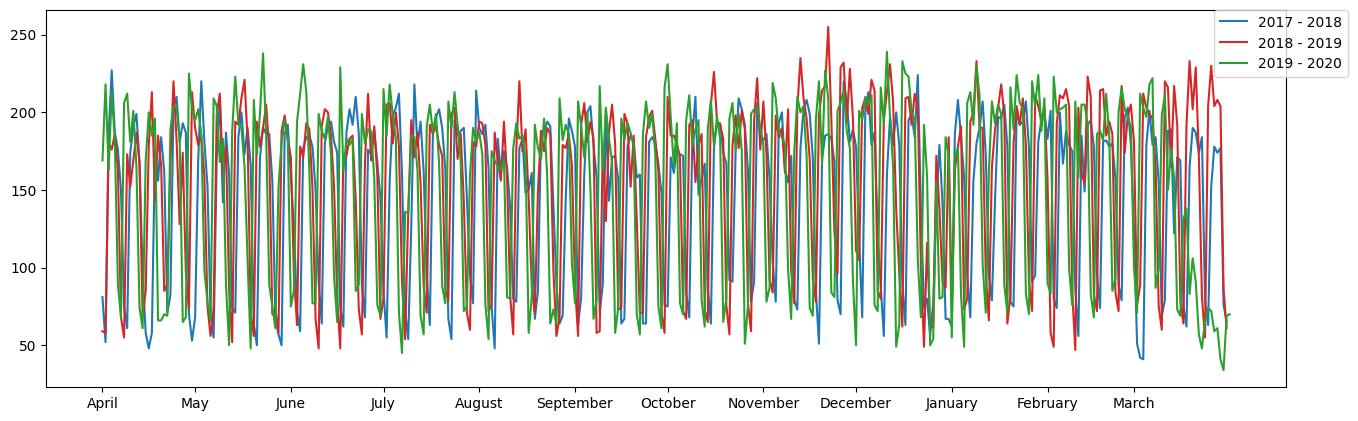
\includegraphics[width=\textwidth]{Chapters/Chapter5/Figures/Admission each year.png}
    \caption{Daily Count of Admissions into ABUHB per year}
    \label{fig:AdmissionCount}
\end{figure}

Due to the COVID-19 pandemic and the skewed effects it would have had on admission statistics, data from April 2020 was excluded from the study \cite{Venkatesan2020}. The effect of COVID-19 can be seen from March 2020, where admissions for patients aged 65 and older had started to decrease.

Within the data there were 66,289 unique NHS numbers, meaning 98,829 stays were either part of a care spell or independent admissions. The data did not give any indication regarding patient care spells, i.e., where they had been transferred between hospitals. Therefore, it was decided that if a patient had been discharged and subsequently readmitted on the same day, then this would fall into the `care spell’ category. In total there were 9,464 care spell episodes. Table \ref{Tab:Spell} displays the number of transfers.

\begin{table}[h!]
    \centering
    \begin{tabular}{cccccccc}\toprule
    \textbf{No. of Transfers} & \textbf{1} & \textbf{2} & \textbf{3} & \textbf{4} & \textbf{5} & \textbf{6} & \textbf{7}   \\ \midrule
\textbf{Total} & 8435 & 313 & 50 & 22 & 4 & 1& 1\\ \bottomrule
    \end{tabular}
    \caption{Number of Patient Transfers}
    \label{Tab:Spell}
\end{table}

The patient who underwent seven transfers and readmissions, spent a total 219 days in hospital, primarily moving between Royal Gwent Hospital (RGH) and County Hospital before being discharged to a non-NHS care home. This is also known as step-up and step-down care.

The age of patients had a lower bound of 65, with the oldest age of 107 years old. The mean age was calculated to be 77 years with a standard deviation of eight years. Due to the 42 year age range, patients were also grouped into five-year age categories to determine if this would be a more accurate predictor (Figure \ref{fig:AgeGroup}). 

\begin{figure}[h!]
    \centering
    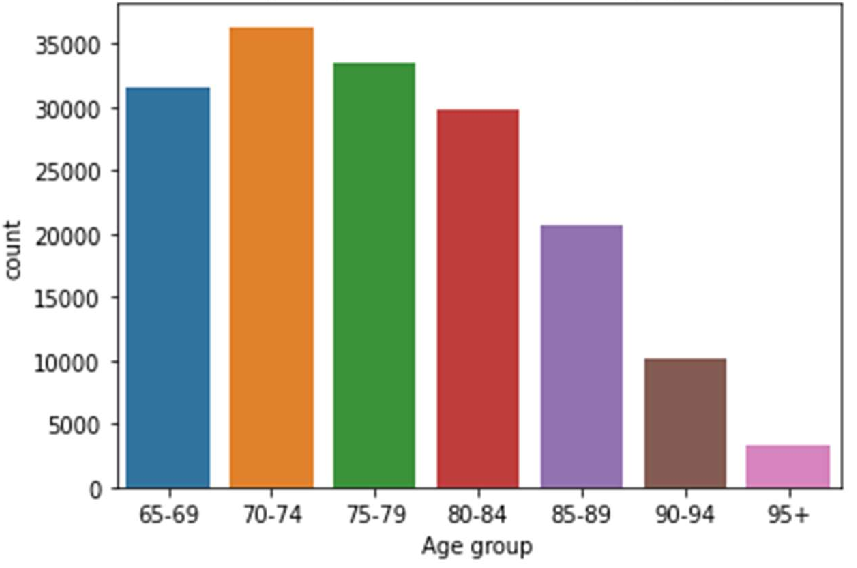
\includegraphics[scale=0.6]{Chapters/Chapter5/Figures/Age group.pdf}
    \caption{Categorical Age of Patients}
    \label{fig:AgeGroup}
\end{figure}

The highest frequency of admissions occurred on a Tuesday (18.04\%), followed by a Thursday (17.84\%) (Figure \ref{fig:AdmissionTimes}). Patients who were admitted over a weekend accounted for 14.08\% of total admissions. Weekday admissions peaked between 7am and 10am, with a secondary peak between 12pm and 1pm.

\begin{figure}[h!]
    \centering
    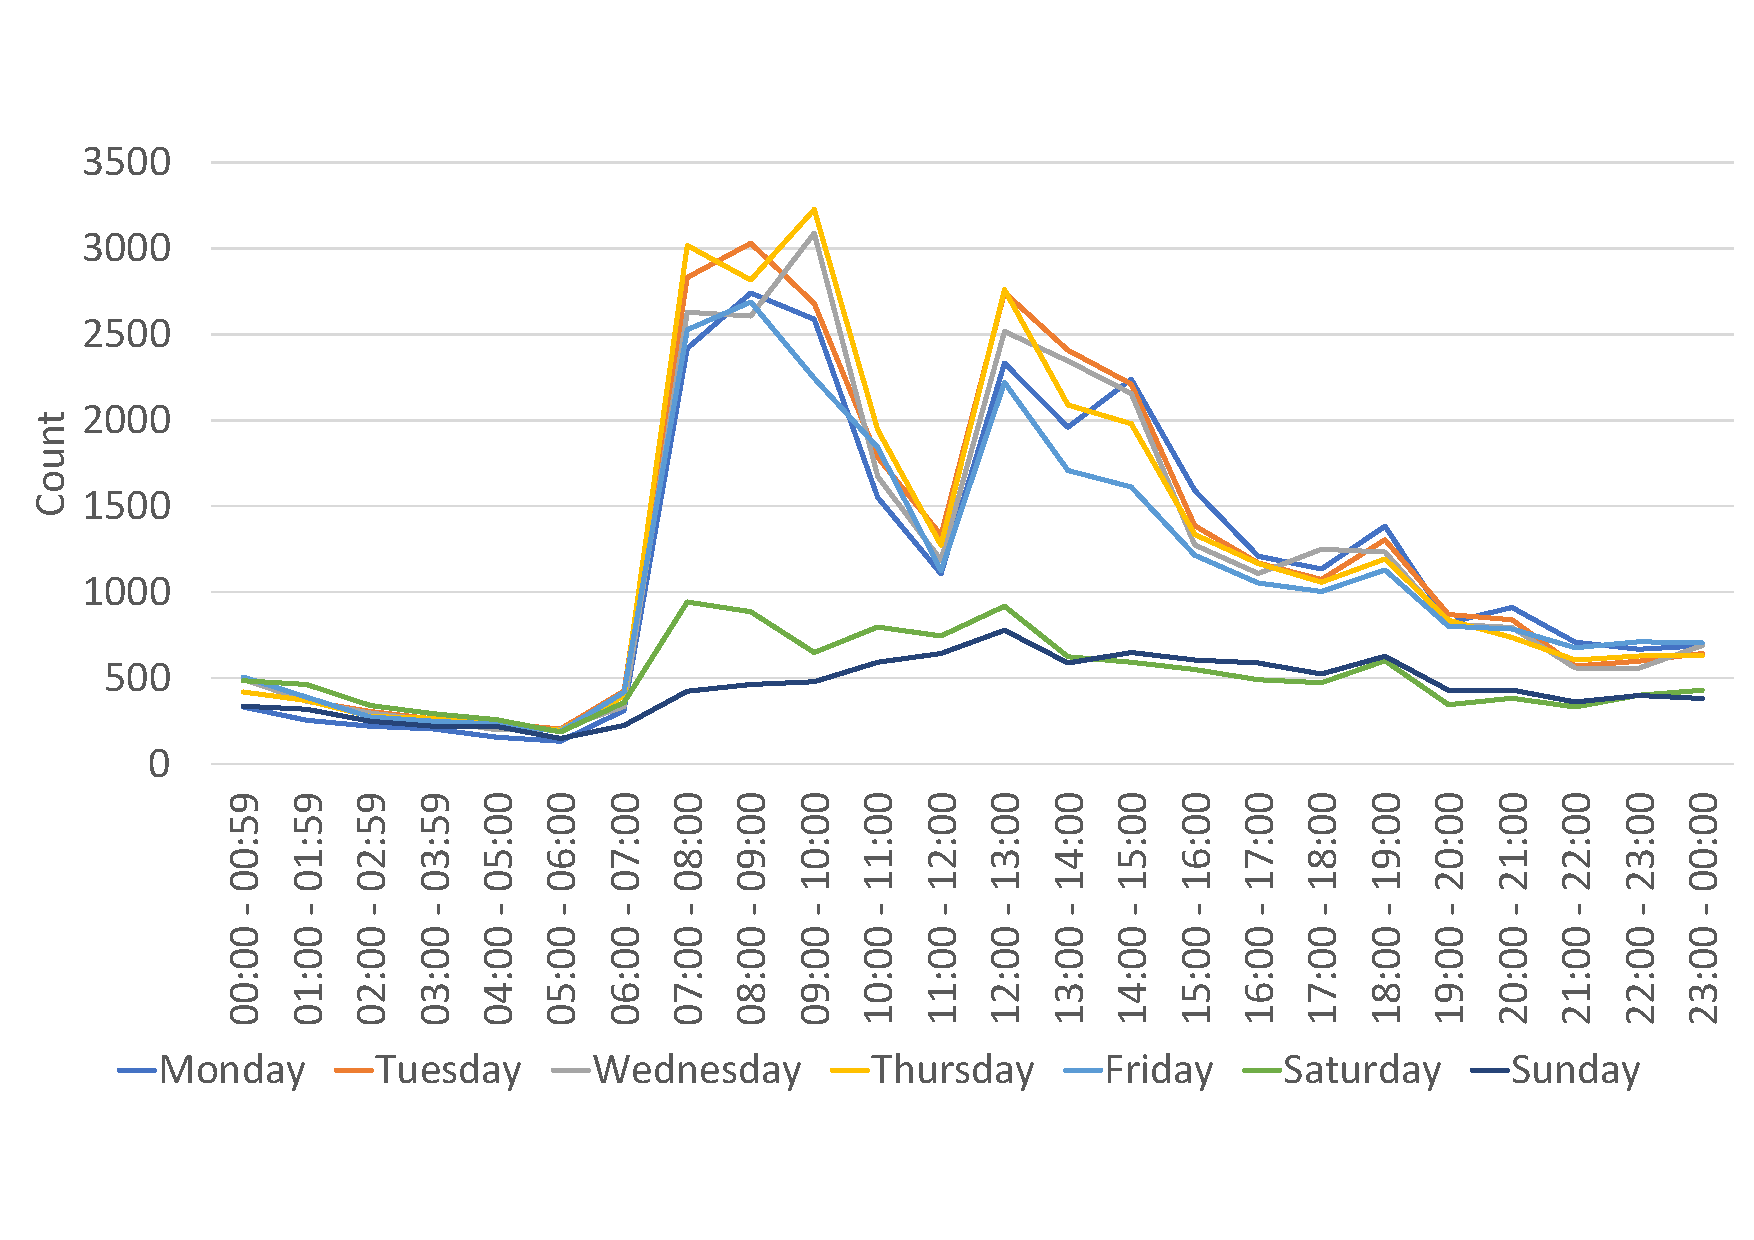
\includegraphics[width=\textwidth]{Chapters/Chapter5/Figures/AdmissionTimes.pdf}
    \caption{Admissions by Hour and Day Interval}
    \label{fig:AdmissionTimes}
\end{figure}

The admission source of a patient determined where a patient was directly prior to admission. Although there are 25 different admission sources listed in total, the top six admission sources accounted for 98.63\% of admissions (Table \ref{tab:AdmissionSource}). If this were to be extended to include the top ten, 99.88\% of admissions would be accounted for. The top two admission sources, `Usual Place of Residence' and `Own Home' have a combined patient count of 147,294 (89.21\%).

\begin{table}[h!]
    \centering
    \begin{tabular}{lcc}\toprule
    \textbf{Admission Source} & \textbf{Count} &\textbf{Proportion} \\ \midrule
    Usual Place of Residence &	99464 & 60.24\% \\
Own Home&	47830 & 28.97\%\\
Same Trust-General or young phys.disabled&	7711 &4.67\%\\
Patient transfer within the same health board/trust	&4350 &2.63\%\\
Non NHS (other then L.A.) run res.care home&	1755 &1.06\%\\
Non NHS (other than L.A.) run nursing home&	1314 &0.80\%\\
 \bottomrule
    \end{tabular}
    \caption{Top Six Admission Sources}
    \label{tab:AdmissionSource}
\end{table}


The admission method followed a similar trend to the admission source, with a small number of methods accounting for the majority of patients. Although there were 16 distinct methods, 99.23\% of patients were accounted for through the top seven (Table \ref{tab:AdmissionMethod}). `Elective - waiting list' was the most common admission method and is one that has been arranged in advance of admission. The patient has been admitted via a waiting list, where at the point of being put on to the waiting list, did not know their date of admission. The period in which the patient has to wait is dependant on the demand for hospital resources and facilities.

\begin{table}[h!]
    \centering
    \begin{tabular}{lcc}\toprule
    \textbf{Admission Method} & \textbf{Count} &\textbf{Proportion} \\ \midrule
Elective - waiting list& 73482 & 44.50\%\\
Emergency - casualty&	39437 &23.88\%\\
Emergency - GP&  	28169&17.06\%\\
Other - transferred from another hospital  & 	13460&8.15\%\\
Elective - booked  &5950 & 3.60\%\\
Elective - planned&1696 & 1.02\%\\
Emergency - other means&1658 & 1.04\%\\
 \bottomrule
    \end{tabular}
    \caption{Top Seven Admission Methods}
    \label{tab:AdmissionMethod}
\end{table}

The LOS of the patient was determined by the time between admission and hospital discharge. There was a large range of LOS's, from 0 to 413 days. The LOS can be modelled in two ways, in hours or in days. The first method of calculating LOS, used the number of hours that patients had been admitted for. It was determined using the admission and discharge dates as well as specific times. The average LOS was calculated to be 155.23 hours (6.47 days). The second method of calculating LOS, meant that if a patient was admitted overnight, an additional day was added to their LOS i.e., if admitted Monday evening and discharged Tuesday morning, their LOS was \hl{CHECK THIS} 2.
\hl{Read up to here}
Further analysing LOS in hours, the mean was 6.47 days, whilst the 75$^{th}$ percentile was 7 days. The 90$^{th}$ percentile was 18 days increasing to 30 with the 95$^{th}$ percentile. This suggests there are some long LOS's that are skewing the mean. 81,538 (49.38\%) of patients were discharged within 24 hours, and 114,015 (69.05\%) patients were discharged within 5 days. 5\% of patients had a LOS greater than 30 days.

Depending on the day admitted, the LOS of a patient varied (Table \ref{tab:DayLOS}). Again, patients who were admitted on a weekend have a different variation to those patients admitted during the week. The average LOS was at least an extra day longer if admitted on a weekend.

\begin{table}[h!]
    \centering
    \begin{tabular}{lcc}\toprule
    \textbf{Day of week} & \textbf{Mean LOS} & \textbf{Standard Deviation}\\    \midrule
    Monday & 6.22 & 12.77\\
    Tuesday & 6.12 & 13.54\\
    Wednesday &6.11 &13.25\\
    Thursday &5.97 & 13.02\\
    Friday &6.78  &12.97\\
    Saturday & 7.88 & 13.78\\
    Sunday & 8.10  &12.97\\ \bottomrule
    \end{tabular}
    \caption{Mean and Standard Deviation of LOS by Admission Day}
    \label{tab:DayLOS}
\end{table}

The frailty score was calculated using two methods both using the ICD10 codes, as discussed in Section \ref{sec:elderlyfrail}. In total there were 2,758 different codes relating to the diagnosis and reason for admission of the patient. The average frailty score was 0.5, with a standard deviation of 0.98. The maximum score was 8.1, with the lowest score being zero.


Patients admitted into hospital can be given multiple scans, depending on their condition and treatment. It was calculated there were 12,350 unique patient stays of which 9,863 patients had one scan only (Table \ref{Tab:Scan}). There were 2,487 patients who had at least two scans, of which 1,957 patients who only had two scans. One patient had a total of eight scans. 

\begin{table}[h!]
    \centering
    \begin{tabular}{lccccccc}\toprule
    \textbf{Scan Number} & \textbf{1} & \textbf{2} & \textbf{3} & \textbf{4} & \textbf{5} & \textbf{6} & \textbf{8}   \\ \midrule
\textbf{Count} & 9863 & 1957 & 437 & 77 & 11 & 4& 1\\ \bottomrule
    \end{tabular}
    \caption{Number of Patients against Number of Scans}
    \label{Tab:Scan}
\end{table}




% \begin{itemize}
%     \item Age
%     \item Hospital
%     \item Admission Times/day
%     \item Locality of arrivals
%     \item Scan data
%     \item no scan patients against scan patients 
%     \item LOS
%     \item frailty
% \end{itemize}

\subsection{Data Insights}
The information from the combined data sets provides 165,118 patient records over a three year period with admissions remaining constant throughout this time. There are a higher concentration of arrivals from populous towns and cities in South East Wales, such as Caerphilly and Newport, with fewer arrivals from remote areas within the region. The higher attended hospitals tended to be the acute hospitals with 24/7 services in the region, similarly located in Caerphilly and Newport. Admissions tend to be higher during the week, with peak admissions arriving on a Tuesday. For all arrivals, there tended to be peaks in the late morning, early afternoon, and a smaller peak in the evening. The patient demographics are varied amongst all hospitals, however the LOS varied by age and hospital attended. The trends show that shorter LOS are more common at acute hospitals with longer LOS's at more community based hospitals. The age of the patients are fairly mixed, however the majority are aged between 65 and 85. The frailty scores of the patients provide some indication on the severity of the illness. For certain hospitals, a higher frailty score is correlated with longer lengths of stays and older age of patients. There were a small subset of admitted patients who require at least one scan within hospital.




% \begin{itemize}
%     \item Keep it brief
%     \item Two data types
%     \item Key results
% \end{itemize}
\section{Predictive Analytics Results}\label{sec:predictiveresults}
This section will look at applying the theory of predictive analytics discussed in Chapter \ref{chp:predictive} to the patient data from ABUHB to determine how clinical and demographic attributed effect hospital LOS.
\subsection{Linear Regression}\label{sec:linregresults}
Linear regression was performed on the fourteen variables to determine the highest influence on LOS. The LOS was converted into how many nights the patient spent in hospital, for example, if admitted on 01/01/2020 and discharged on 03/01/2020, the LOS would be three. This produced a higher R$^{2}$ value for linear regression for all cases than using the continuous hourly LOS. Table\ref{Tab:ContinuousLOS-Lin}, displays both the R$^{2}$ and adjusted R$^{2}$ values for each variable against this LOS.



\begin{table}[h!]
\centering\scalebox{1}{
\begin{tabular}{lcc}
\toprule
\textbf{Continuous Variables} & \textbf{R$^2$ Value}&\textbf{Adjusted R$^2$ Value} \\ \midrule 
Age & 0.050 & 0.050 \\
Frailty Score & 0.028 & 0.028 \\
No. of Scans & 0.003 & 0.003 \\ \midrule
\textbf{Categorical Variables} & \textbf{R$^2$ Value}&\textbf{Adjusted R$^2$ Value} \\ \midrule
Age Group &  0.051 & 0.051 \\
Admission Method & 0.282 & 0.282  \\
Admission Source & 0.195 & 0.195 \\
Day of Admission & 0.002& 0.002\\
Diagnosis & 0.273 & 0.261\\
Frailty Group & 0.028& 0.028\\
Hospital & 0.182 & 0.181 \\
ICD10 - First Letter & 0.092& 0.092\\
Scan Y/N & 0.002 & 0.002 \\
Month of Admission & 0.000& 0.000\\
Specialty & 0.288 & 0.288\\\bottomrule
\end{tabular}}
\caption{Linear Regression Result}
\label{Tab:ContinuousLOS-Lin}
\end{table}

The variables can be considered as two different data types, continuous and categorical. Within the continuous variables, age produced the highest R$^{2}$ value of 0.05. This means 5\% of the LOS variation is explained by Age. The model can be denoted by: 
\begin{equation}
    Y = 0.375x - 22.635
\end{equation}
where $x$ is the age of the patient.
Therefore, for each 1 year increment in age, the LOS will increase by 0.375 days.

Similarly, we can calculate the linear regression model for categorical variables within Table \ref{Tab:ContinuousLOS-Lin}. The month of admission, produced an R$^{2}$ value of zero, meaning that month explains none of the variability of the response data around its mean. Specialty provided the largest R$^{2}$ value of 0.288. Within the specialty category, there are 29 subcategories of different specialities. In order to be able to predict LOS, we can further analyse each variable. Table \ref{tab:linreg-specialty} denotes the associated linear regression values for specialty. When one $x$ variable is selected, the corresponding value is the LOS. For example, if the specialty of A\&E is chosen, the LOS will be 2.2673 days. This can be directly compared to other specialties, for example Anaesthetics has a LOS of 6.5 times longer than A\&E. The value column displays the variation in the average LOS between each of the specialties.

% where $x_{1}$ = Accident \& Emergency, $x_{2}$ = Anaesthetics, $x_{3}$ = Cardiology, $x_{4}$ = Care of the Elderly, $x_{5}$ = Community Medicine, $x_{6}$ = Dermatology, $x_{7}$ = Diabetes \& Endocrinology, $x_{8}$ = Ear, Nose \& Throat, $x_{9}$ = GP Other, $x_{10}$ = Gastroenterology, $x_{11}$ = General Medicine, $x_{12}$ = General Surgery, $x_{13}$ = Gynaecology, $x_{14}$ = Haematology, $x_{15}$ = Infectious Diseases, $x_{16}$ = Intermediate Care, $x_{17}$ = Maxillo-Facial, $x_{18}$ = Neurology, $x_{19}$ = Opthalmology, $x_{20}$ = Pain, $x_{21}$ = Plastic Surgery, $x_{22}$ = Radiology, $x_{23}$ = Radiotherapy \& Oncology, $x_{24}$ = Rehabilitation, $x_{25}$ = Respiratory, $x_{26}$ = Restorative Dentistry, $x_{27}$ = Rheumatology, $x_{28}$ = Trauma \& Orthopaedic ,$x_{29}$ = Urology.\\
% \begin{align}
%     Y =& 2.2673x_1 + 14.9517x_2 +4.647x_3 +12.1101x_4 + 34.235x_5 +0.2616x_6 +\nonumber \\  &11.6161x_7+
%     2.75x_8 +39.2603x_9 + 2.1382x_{10} +8.4519x_{11} + 3.7149x_{12} +\nonumber\\ &1.6536x_{13} + 0.7974x_{14} + 
%     11.6289x_{15} + 14.3725x_{16} + 0.6018x_{17} + 5.6131x_{18}+\nonumber\\ 
%      &0.1307x_{19} + 0.0080x_{20} + 0.1128x_{21} + 0.3548x_{22} + 13.6667x_{23} + 28.7732x_{24} + \nonumber\\ 
%      &7.7985x_{25} + 0x_{26} + 2.3333x_{27} + 6.6658x_{28} + 0.9932x_{29}
% \end{align}


\begin{table}[h!]
    \centering
    \begin{tabular}{lcc} \toprule
      Specialty Type   & $x$ Variable & Value \\ \midrule
      Accident \& Emergency (A\&E) & $x_{1}$ & 2.2673\\ 
      Anaesthetics & $x_{2}$ & 14.9517 \\
      Cardiology & $x_{3}$ & 4.647\\
      Care of the Elderly & $x_{4}$ & 12.1101 \\
      Community Medicine & $x_{5}$ & 34.235\\
      Dermatology & $x_{6}$ & 0.2616\\
      Diabetes \& Endocrinology & $x_{7}$ & 11.6161\\
      Ear, Nose \& Throat & $x_{8}$ &2.75 \\
      GP Other & $x_{9}$ & 39.2603\\
      Gastroenterology & $x_{10}$ &2.1382 \\
      General Medicine & $x_{11}$ & 8.4519\\
      General Surgery & $x_{12}$ & 3.7149\\
      Gynaecology & $x_{13}$ & 1.6536\\
      Haematology & $x_{14}$ & 0.7974\\
      Infectious Diseases & $x_{15}$ &11.6289 \\
      Intermediate Care & $x_{16}$ &14.3725 \\
      Maxillo-Facial & $x_{17}$ & 0.6018\\
      Neurology & $x_{18}$ & 5.6131 \\
      Opthalmology & $x_{19}$ &0.1307 \\
      Pain & $x_{20}$ & 0.0080\\
      Plastic Surgery & $x_{21}$ & 0.1128\\
      Radiology & $x_{22}$ & 0.3548\\
      Radiotherapy \& Oncology & $x_{23}$ & 13.6667\\
      Rehabilitation & $x_{24}$ & 28.7732\\
      Respiratory & $x_{25}$ & 7.7985\\
      Restorative Dentistry & $x_{26}$ & 0\\
      Rheumatology & $x_{27}$ & 2.3333\\
      Trauma \& Orthopaedic & $x_{28}$ & 6.6658\\
      Urology & $x_{29}$ &0.9932 \\\bottomrule
    \end{tabular}
    \caption{Linear Regression Results - Specialty}
    \label{tab:linreg-specialty}
\end{table}

\newpage
\subsection{Logistic Regression}\label{sec:logregresults}
Logistic regression was performed to determine the effect of grouping LOS. Grouped LOS categories was determined by grouping patients into whether they were discharged on the same day as arrival or admitted overnight. This resulted in 75,216 patients falling into the `0' category (45.55\%), where they were discharged the same day and 89,902 patients who fell into the `1' category (54.45\%) where their LOS was at least 2 days. This is beneficial for bed and staff planning to determine the turnaround time of patients. 

Table \ref{Tab:ContinuousLOS-Log} displays the four scoring measures against each of the variables. In three cases, precision is given the value `N/A', this is due to both the TP and FP rates both being zero (i.e., the model only predicted negative results). Therefore, a result cannot be calculated. Similarly, because the precision cannot be calculated, then the F1 score cannot be calculated.

\begin{table}[h!]
\centering\scalebox{1}{
\begin{tabular}{lcccc}
\toprule
{\textbf{Continuous Variables}} &\textbf{Accuracy}& \textbf{Precision} & \textbf{Recall} & \textbf{F1 Score}\\ \midrule
Age  & 0.6037 &0.5721 & 0.5164 & 0.5428\\
Frailty Score  & 0.5860 & 0.5283 & 0.8503 & 0.6517\\
No. of Scans & 0.5445 & N/A & 0.0 & N/A\\
\midrule
{\textbf{Categorical Variables}} &\textbf{Accuracy}& \textbf{Precision} & \textbf{Recall} & \textbf{F1 Score}\\ \midrule
Age Group & 0.6037 & 0.5721 & 0.5164 & 0.5428\\
Admission Method & 0.8764 &0.8378 & 0.9036 & 0.8694 \\
Admission Source & 0.5829 & 1.0 & 0.0844 & 0.1557 \\
Day of Admission & 0.5474 & 0.5085 & 0.1991 & 0.2862\\
Diagnosis  & 0.8496 & 0.8360 & 0.8607 & 0.8481 \\
Frailty Group  & 0.5871 &0.5291 & 0.8498 & 0.6522\\
Hospital& 0.6171 & 0.6923 & 0.2871 & 0.4059 \\
ICD10 - First Letter & 0.7554 & 0.7813 & 0.6430 & 0.7055 \\
Scan Y/N & 0.4555 & N/A& 0.0 & N/A\\
Month of Admission & 0.4555 & N/A& 0.0 & N/A \\
Specialty & 0.8008 & 0.7645 & 0.8131 & 0.7881 \\\bottomrule
\end{tabular}}
\caption{Logistic Regression Result}
\label{Tab:ContinuousLOS-Log}
\end{table}

We can determine the likelihood of falling into one of the two LOS groupings using the logit function. Equation \ref{eq:logit} displayed the general formula using age, a continuous variable, as an example.
\begin{equation}\label{eq:logit}
    logit(\pi(x)) = \ln\left[ \frac{\pi(x)}{(1-\pi(x))}\right] = -5.0746 +0.0681*Age
\end{equation}
If age is set to be 80, then the conditional logit of being admitted overnight is:
\begin{equation}
    \ln\left[\frac{\pi(x)}{(1-\pi(x))}\right](Age =80) = -5.0746 +0.0681*80 
\end{equation}
Then the effect of a one-unit increase in age can be examined. When the age of a patient is 81,
\begin{equation}
    \ln\left[\frac{\pi(x)}{(1-\pi(x))}\right](Age = 71) = -5.0746 +0.0681*81 
\end{equation}
Taking the difference of the two equations, we are left with the following result:
\begin{equation}
\ln\left[\frac{\pi(x)}{(1-\pi(x))}\right](Age =81) - \ln\left[\frac{\pi(x)}{(1-\pi(x))}\right](Age = 80) = 0.1381
\end{equation}
Therefore the coefficient for age is the difference in the log odds, and as such, for one unit increase in age, the expected change in log odds is 0.1381. Exponentiating both sides, results in a value of 1.1481:
\begin{equation}
    e^{\ln\left[\frac{\pi(x)}{(1-\pi(x))}\right](Age =81) - \ln\left[\frac{\pi(x)}{(1-\pi(x)}\right](Age = 80)} = e^{0.1381} = 1.1481
\end{equation}

Therefore we can say for one-unit increase in age, there is a 14.81\% increase in the odds of being admitted overnight. The 14.81\% of increase is not dependent on the value age is held at.
%https://stats.oarc.ucla.edu/other/mult-pkg/faq/general/faq-how-do-i-interpret-odds-ratios-in-logistic-regression/

%https://quantifyinghealth.com/interpret-logistic-regression-coefficients/#:~:text=Interpret%20Logistic%20Regression%20Coefficients%20%5BFor%20Beginners%5D%201%201.,light%20smoker%2C%202%3A%20moderate%20smoker%2C%203%3A%20heavy%20smoker%29

Similarly, we can calculate the log odds for a categorical variable, e.g., age group. Table \ref{tab:logisticregcat} describes the relationship between LOS group and age group.

\begin{table}[h!]
    \centering
    \begin{tabular}{ccc}\toprule
    \textbf{Age Group} & \textbf{Log Odds Ratio} &\textbf{Odds compared to 65-69} \\ \midrule
       Intercept  & -0.3582 & -\\
       70-74 & 0.1263 & 13.46\%\\
       75-79 & 0.4389 & 55.10\%\\
       80-84 & 0.7609 &114.02\%\\
       85-89 & 1.2366 & 244.39\%\\
       90-94 & 1.8219& 518.36\%\\
       95+ & 2.2298& 829.80\%\\ \bottomrule
    \end{tabular}
    \caption{Log Odds Ratio against Age Group}
    \label{tab:logisticregcat}
\end{table}
The intercept is also known as the reference category, which in this instance is the age group `65-69'. If we compare the reference group to the `70-79' category and perform, $e^{0.1263}$, a result of 1.1346 is produced. This shows that patients in the `70-74' age group have a 13.46\% higher chance of being admitted overnight. There is an 829.80\% higher chance of 95+ year old patient being admitted compared to those aged between 65 and 69.





\subsection{Classification and Regression Trees}
The variables analysed within subsections \ref{sec:linregresults} and \ref{sec:logregresults} can then be inputted into CART models to predict patients LOS within hospitals. Diagnosis will be used instead of the `ICD10 - first letter', since both linear and logistic regression results produced a higher result. Similarly, the number of scans rather than whether a person had a scan (Scan Y/N), will be used. Age and age group will be investigated on their impact on the CART model. To determine the effect of using a frailty measure, continuous, grouped frailty will be compared against not using a frailty score within the model.

\subsubsection{Regression Trees}\label{sec:regressiontrees}
This section will look at the development and results of the regression trees, analysing continuous LOS. A total of nine variables will be used within the model, listed as follows:
\begin{multicols}{2}
\begin{itemize}
    \item Admission Method
    \item Admission Source
    \item Age (Continuous and Grouped)
    \item Day
    \item Diagnosis
    \item Frailty (None, Continuous and Grouped)
    \item Hospital
    \item Number of Scans
    \item Specialty
\end{itemize}
\end{multicols}

Month was excluded from the regression model since in the linear regression model the R$^{2}$ was calculated to be zero and therefore did not account for any of the variability in patients LOS.

A 20\% test set was used, meaning the data is trained on 80\% of the data. Using the Python algorithm discussed in Section \ref{sec:pythonreg}, Table \ref{tab:ParametersRegression} displays the parameters inputted into the model. The parameters `min\_samples\_leaf' and `max\_leaf\_nodes' will undergo testing to determine the trade off between R$^{2}$ score and computation time.

%iterative process for selecting optimum parameters in function

\begin{table}[h!]
    \centering
    \begin{tabular}{lc} \toprule
        \textbf{Parameters} & \textbf{DecisionTreeRegressor} \\\midrule
         criterion& ``squared\_error''\\
         splitter & ``best'' \\
         max\_depth & None \\
         min\_samples\_split & 2 \\
         min\_weight\_fraction\_leaf & 0 \\
         max\_features & None \\
         random\_state & None \\
         min\_impurity\_decrease & 0 \\
         ccp\_alpha & 0 \\\bottomrule
    \end{tabular}
    \caption{Selected Parameters for `DecisionTreeRegressor'}
    \label{tab:ParametersRegression}
\end{table}

Tables \ref{tab:regtree1a} - \ref{tab:regtree6c} display the R$^{2}$ score and computation time for a range of `max\_leaf\_nodes' and `min\_samples\_leaf' variables.  The variable `max\_leaf\_nodes' was tested on a range from five to 30 leaf nodes. Larger values were not selected to ensure a usable number of groups were identified. The variable `min\_samples\_leaf', was investigated from one sample to 500 samples. By having a minimum number of samples per leaf, in theory will reduce the likelihood of overfitting. Computation time was also collected to determine if there was a trade off between R$^{2}$ and time to run the model.

The highest R$^{2}$ score of 34.28\% was attained in the regression tree using grouped age and continuous frailty (Table \ref{tab:regtree5a}). This was achieved using 100 minimum samples per leaf and 30 maximum leaf nodes. However, in comparison to other models, it produced a longer computation run time of 26.9786 seconds (Table \ref{tab:regtree5c}). If analysing on the grouped age and continuous frailty models, by reducing R$^{2}$ by 0.05\%, approximately 6.9 seconds can be saved by increasing the number of minimum samples per leaf to 200. 

Within Table \ref{tab:regtree6a}, 30 maximum leaf nodes and 100 minimum samples per leaf also produced an R$^{2}$ score of 34.23\%, with a computational time of 18.5107 seconds. This combination was selected as the optimum and will be used going forward as it produces a large R$^{2}$ score with low computation time.

The R$^{2}$ scores all range between 29.25\% to 34.28\%, due to the large range of LOS's within the data. The range of LOS was between 0 days and 417 days, and an R$^{2}$ score of 34\%, shows 34\% of the time we are able to correctly assign patients to the correct node, despite this large range. These leaf nodes, will be able to used to group patients accordingly to LOS.


\begin{landscape}

\begin{table}[h!]
\begin{subtable}{.45\linewidth}
    \centering\scalebox{0.8}{
    \begin{tabular}{cccccccc}\toprule
    & \multicolumn{7}{c}{\textbf{min\_samples\_leaf}}\\
	&&\textbf{1} &	\textbf{100}	&\textbf{200}&	\textbf{300}&	\textbf{400}&	\textbf{500}\\\midrule
\parbox[t]{2mm}{\multirow{6}{*}{\rotatebox[origin=c]{90}{\textbf{max\_leaf\_nodes}}}} & \textbf{5}	& \g{0.2925}	&\g{0.2925} &\g{0.2925}&\g{0.2925} & \g{0.2925}&\g{0.2925} \\
&\textbf{10}	& \g{0.3224}	&\g{0.3224} &\g{0.3224}&\g{0.3190} & \g{0.3190}&\g{0.3190} \\
&\textbf{15}	& \g{0.3328}	&\g{0.3328} &\g{0.3328}&\g{0.3322} & \g{0.3322}&\g{0.3250} \\
&\textbf{20}	& \g{0.3362}	&\g{0.3384} &\g{0.3384}&\g{0.3374} & \g{0.3374}&\g{0.3286} \\
&\textbf{25}	& \g{0.3377}	&\g{0.3408} &\g{0.3408}&\g{0.3393} & \g{0.3392}&\g{0.3301} \\
&\textbf{30}	& \g{0.3375}	&\g{0.3416} &\g{0.3410}&\g{0.3395} & \g{0.3407}&\g{0.3304} \\\bottomrule

    \end{tabular}}
    \caption{R$^{2}$ score}
    \label{tab:regtree1a}
    \end{subtable}
\begin{subtable}{.45\linewidth}

    
    \centering\scalebox{0.8}{
    \begin{tabular}{cccccccc}\toprule
    & \multicolumn{7}{c}{\textbf{min\_samples\_leaf}}\\
	&&\textbf{1} &	\textbf{100}	&\textbf{200}&	\textbf{300}&	\textbf{400}&	\textbf{500}\\\midrule
\parbox[t]{2mm}{\multirow{6}{*}{\rotatebox[origin=c]{90}{\textbf{max\_leaf\_nodes}}}} & \textbf{5}	& \ga{9.5668} & \ga{9.8238} & \ga{9.7276} & \ga{8.5625} & \ga{8.5016} & \ga{8.8017}\\
& \textbf{10} & \ga{13.9514} & \ga{12.0725} & \ga{11.9836} & \ga{11.9235} & \ga{13.9066} & \ga{12.6438} \\
& \textbf{15} & \ga{14.4875} & \ga{14.2050} & \ga{16.7100} & \ga{14.2829} & \ga{14.5327} & \ga{14.8251} \\
& \textbf{20} & \ga{16.7751} & \ga{17.9756} & \ga{16.5835} & \ga{15.8724} & \ga{15.6849} & \ga{14.9515} \\
& \textbf{25} & \ga{17.8356} & \ga{18.2084} & \ga{16.8472} & \ga{16.8951} & \ga{17.8183} & \ga{18.5711} \\
& \textbf{30} & \ga{19.5540} & \ga{19.1484} & \ga{19.1552} & \ga{18.5376} & \ga{19.4121} & \ga{19.6245} \\\bottomrule

    \end{tabular}}
    \caption{Computational Time in Seconds (s)}
    \label{tab:regtree1c}

\end{subtable}
\label{tab:regtree1}
\caption{Regression Tree R$^{2}$ and Computational Time Results - Continuous Age and No Frailty}
\end{table}




\begin{table}[h!]
\begin{subtable}{.45\linewidth}
    \centering\scalebox{0.8}{
    \begin{tabular}{cccccccc}\toprule
    & \multicolumn{7}{c}{\textbf{min\_samples\_leaf}}\\
	&&\textbf{1} &	\textbf{100}	&\textbf{200}&	\textbf{300}&	\textbf{400}&	\textbf{500}\\\midrule
\parbox[t]{2mm}{\multirow{6}{*}{\rotatebox[origin=c]{90}{\textbf{max\_leaf\_nodes}}}} & \textbf{5}	& \g{0.2925}& \g{0.2925} & \g{0.2925} & \g{0.2925} & \g{0.2925} & \g{0.2925} \\
&\textbf{10} & \g{0.3224} & \g{0.3224} & \g{0.3224} & \g{0.3190} & \g{0.3190} & \g{0.3190}\\
&\textbf{15} & \g{0.3328} & \g{0.3328} & \g{0.3328} & \g{0.3322} & \g{0.3322} & \g{0.3250}\\
&\textbf{20} & \g{0.3362} & \g{0.3381} & \g{0.3381} & \g{0.3381} & \g{0.3381} & \g{0.3294}\\
&\textbf{25} & \g{0.3389} & \g{0.3412} & \g{0.3412} & \g{0.3391} & \g{0.3396} & \g{0.3308}\\
&\textbf{30} & \g{0.3383} & \g{0.3420} & \g{0.3422} & \g{0.3393} & \g{0.3410} & \g{0.3308}  \\\bottomrule

    \end{tabular}}
    \caption{R$^{2}$ Score}
    \label{tab:regtree2a}
    \end{subtable}
\begin{subtable}{.45\linewidth}

    
    \centering\scalebox{0.8}{
    \begin{tabular}{cccccccc}\toprule
    & \multicolumn{7}{c}{\textbf{min\_samples\_leaf}}\\
	&&\textbf{1} &	\textbf{100}	&\textbf{200}&	\textbf{300}&	\textbf{400}&	\textbf{500}\\\midrule
\parbox[t]{2mm}{\multirow{6}{*}{\rotatebox[origin=c]{90}{\textbf{max\_leaf\_nodes}}}} & \textbf{5}	& \ga{8.9660} & \ga{9.1705}	& \ga{8.7471} & \ga{8.4058}	& \ga{8.7663} & \ga{8.4657}\\
& \textbf{10} & \ga{12.9853} & \ga{12.1247}	& \ga{11.7582}	& \ga{11.6642}	& \ga{15.0279}	& \ga{12.1618}\\
& \textbf{15} & \ga{13.4786} & \ga{13.3782}	& \ga{16.3377}	& \ga{14.3459}	& \ga{15.3793}	& \ga{17.0997}\\
& \textbf{20} & \ga{16.8013} & \ga{18.5770}	& \ga{17.1018}	& \ga{15.8003}	& \ga{16.1066}	& \ga{20.7639}\\
& \textbf{25} & \ga{18.3142} & \ga{17.3414}	& \ga{17.3936}	& \ga{17.6433}	& \ga{25.1619}	& \ga{17.0871}\\
& \textbf{30} & \ga{19.5150} & \ga{18.2041}	& \ga{19.6589}	& \ga{18.7183}	& \ga{20.5239}	& \ga{19.4184}\\\bottomrule

    \end{tabular}}
    \caption{Computational Time in Seconds (s)}
    \label{tab:regtree2c}

\end{subtable}
\label{tab:regtree2}
\caption{Regression Tree R$^{2}$ and Computational Time Results - Continuous Age and Continuous Frailty}
\end{table}


\begin{table}[h!]
\begin{subtable}{.45\linewidth}
    \centering\scalebox{0.8}{
    \begin{tabular}{cccccccc}\toprule
    & \multicolumn{7}{c}{\textbf{min\_samples\_leaf}}\\
	&&\textbf{1} &	\textbf{100}	&\textbf{200}&	\textbf{300}&	\textbf{400}&	\textbf{500}\\\midrule
\parbox[t]{2mm}{\multirow{6}{*}{\rotatebox[origin=c]{90}{\textbf{max\_leaf\_nodes}}}} & \textbf{5}	& \g{0.2925} & \g{0.2925} & \g{0.2925} & \g{0.2925} & \g{0.2925} & \g{0.2925} \\
&\textbf{10} & \g{0.3224} & \g{0.3224} & \g{0.3224} & \g{0.3190} & \g{0.3190} & \g{0.3190}\\
&\textbf{15} & \g{0.3328} & \g{0.3328} & \g{0.3328} & \g{0.3322} & \g{0.3322} & \g{0.3250} \\
&\textbf{20} & \g{0.3362} & \g{0.3384} & \g{0.3384} & \g{0.3379} & \g{0.3379} & \g{0.3291}\\
&\textbf{25} & \g{0.3387} & \g{0.3409} & \g{0.3409} & \g{0.3394} & \g{0.3393} & \g{0.3305} \\
&\textbf{30} & \g{0.3380} & \g{0.3416} & \g{0.3421} & \g{0.3395} & \g{0.3408} & \g{0.3306} \\\bottomrule

    \end{tabular}}
    \caption{R$^{2}$ Score}
    \label{tab:regtree3a}
    \end{subtable}
\begin{subtable}{.45\linewidth}

    
    \centering\scalebox{0.8}{
    \begin{tabular}{cccccccc}\toprule
    & \multicolumn{7}{c}{\textbf{min\_samples\_leaf}}\\
	&&\textbf{1} &	\textbf{100}	&\textbf{200}&	\textbf{300}&	\textbf{400}&	\textbf{500}\\\midrule
\parbox[t]{2mm}{\multirow{6}{*}{\rotatebox[origin=c]{90}{\textbf{max\_leaf\_nodes}}}} & \textbf{5} & \ga{9.5461} & \ga{13.3577} & \ga{10.0347} & \ga{14.3069} & \ga{15.3515} & \ga{10.3998}\\
& \textbf{10} & \ga{12.8929} & \ga{17.2952} & \ga{13.9642} & \ga{13.3573} & \ga{19.6081} & \ga{17.3906}\\
& \textbf{15} & \ga{15.0100} & \ga{20.8186} & \ga{15.0045} & \ga{14.3649} & \ga{17.6949} & \ga{19.1605} \\
& \textbf{20} & \ga{18.6414} & \ga{17.8904} & \ga{17.3192} & \ga{18.0861} & \ga{18.5902} & \ga{15.8897} \\
& \textbf{25} & \ga{24.3819} & \ga{19.3318} & \ga{18.1902} & \ga{19.8152} & \ga{19.1655} & \ga{17.1851} \\
& \textbf{30} & \ga{30.6406} & \ga{24.9834} & \ga{19.9453} & \ga{27.4008} & \ga{24.1919} & \ga{19.1556}\\\bottomrule

    \end{tabular}}
    \caption{Computational Time in Seconds (s)}
    \label{tab:regtree3c}

\end{subtable}
\label{tab:regtree3}
\caption{Regression Tree R$^{2}$ and Computational Time Results - Continuous Age and Grouped Frailty}
\end{table}

\begin{table}[h!]
\begin{subtable}{.45\linewidth}
    \centering\scalebox{0.8}{
    \begin{tabular}{cccccccc}\toprule
    & \multicolumn{7}{c}{\textbf{min\_samples\_leaf}}\\
	&&\textbf{1} &	\textbf{100}	&\textbf{200}&	\textbf{300}&	\textbf{400}&	\textbf{500}\\\midrule
\parbox[t]{2mm}{\multirow{6}{*}{\rotatebox[origin=c]{90}{\textbf{max\_leaf\_nodes}}}} & \textbf{5}	& \g{0.2925} & \g{0.2925} & \g{0.2925} & \g{0.2925} & \g{0.2925} & \g{0.2925} \\
&\textbf{10} & \g{0.3208} & \g{0.3208} & \g{0.3208} & \g{0.3194} & \g{0.3194} & \g{0.3194} \\
&\textbf{15} & \g{0.3320} & \g{0.3208} & \g{0.3320} & \g{0.3320} & \g{0.3320} & \g{0.3236}  \\
&\textbf{20} & \g{0.3347} & \g{0.3379} & \g{0.3379} & \g{0.3369} & \g{0.3369} & \g{0.3292} \\
&\textbf{25} & \g{0.3360} & \g{0.3407} & \g{0.3407} & \g{0.3392} & \g{0.3388} & \g{0.3297} \\
&\textbf{30} & \g{0.3364} & \g{0.3418} & \g{0.3420} & \g{0.3403} & \g{0.3400} & \g{0.3309} \\\bottomrule

    \end{tabular}}
    \caption{R$^{2}$ Score}
    \label{tab:regtree4a}
    \end{subtable}
\begin{subtable}{.45\linewidth}

    
    \centering\scalebox{0.8}{
    \begin{tabular}{cccccccc}\toprule
    & \multicolumn{7}{c}{\textbf{min\_samples\_leaf}}\\
	&&\textbf{1} &	\textbf{100}	&\textbf{200}&	\textbf{300}&	\textbf{400}&	\textbf{500}\\\midrule
\parbox[t]{2mm}{\multirow{6}{*}{\rotatebox[origin=c]{90}{\textbf{max\_leaf\_nodes}}}} & \textbf{5} &\ga{11.6459} & \ga{10.0844} & \ga{12.8503} & \ga{11.3010} & \ga{12.5443} & \ga{9.3685} \\
& \textbf{10} & \ga{14.0654} & \ga{17.3290} & \ga{12.4793} & \ga{17.8037} & \ga{17.7200} & \ga{14.2252} \\
& \textbf{15} & \ga{15.5847} & \ga{19.5658} & \ga{13.5358} & \ga{19.3913} & \ga{15.1067} & \ga{18.1730} \\
& \textbf{20} & \ga{22.4814} & \ga{27.2284} & \ga{20.0218} & \ga{24.0735} & \ga{19.1546} & \ga{19.2974}\\
& \textbf{25} & \ga{20.0251} & \ga{22.6745} & \ga{23.6449} & \ga{23.4709} & \ga{24.0338} & \ga{22.2256}\\
& \textbf{30} & \ga{23.8315} & \ga{24.2733} & \ga{23.7499} & \ga{26.3434} & \ga{20.2900} & \ga{23.4050}\\\bottomrule

    \end{tabular}}
    \caption{Computational Time in Seconds (s)}
    \label{tab:regtree4c}

\end{subtable}
\label{tab:regtree4}
\caption{Regression Tree R$^{2}$ and Computational Time Results - Grouped Age and No Frailty}
\end{table}

\begin{table}[h!]
\begin{subtable}{.45\linewidth}
    \centering\scalebox{0.8}{
    \begin{tabular}{cccccccc}\toprule
    & \multicolumn{7}{c}{\textbf{min\_samples\_leaf}}\\
	&&\textbf{1} &	\textbf{100}	&\textbf{200}&	\textbf{300}&	\textbf{400}&	\textbf{500}\\\midrule
\parbox[t]{2mm}{\multirow{6}{*}{\rotatebox[origin=c]{90}{\textbf{max\_leaf\_nodes}}}} & \textbf{5}	&\g{0.2925} & \g{0.2925} & \g{0.2925} & \g{0.2925} & \g{0.2925} & \g{0.2925} \\
&\textbf{10} & \g{0.3208} & \g{0.3208} & \g{0.3208} & \g{0.3194} & \g{0.3194} & \g{0.3194} \\
&\textbf{15} & \g{0.3320} & \g{0.3208} & \g{0.3320} & \g{0.3320} & \g{0.3320} & \g{0.3236} \\
&\textbf{20} & \g{0.3286} & \g{0.3384} & \g{0.3384} & \g{0.3377} & \g{0.3377} & \g{0.3294} \\
&\textbf{25} & \g{0.3321} & \g{0.3417} & \g{0.3417} & \g{0.3403} & \g{0.3397} & \g{0.3309} \\
&\textbf{30} & \g{0.3314} & \g{0.3428} & \g{0.3423} & \g{0.3402} & \g{0.3409} & \g{0.3322} \\\bottomrule

    \end{tabular}}
    \caption{R$^{2}$ Score}
    \label{tab:regtree5a}
    \end{subtable}
\begin{subtable}{.45\linewidth}

    
    \centering\scalebox{0.8}{
    \begin{tabular}{@{}cccccccc@{}}\toprule
    & \multicolumn{7}{c}{\textbf{min\_samples\_leaf}}\\
	&&\textbf{1} &	\textbf{100}	&\textbf{200}&	\textbf{300}&	\textbf{400}&	\textbf{500}\\\midrule
\parbox[t]{2mm}{\multirow{6}{*}{\rotatebox[origin=c]{90}{\textbf{max\_leaf\_nodes}}}} & \textbf{5}	& \ga{10.3076} & \ga{13.7601} & \ga{13.3941} & \ga{10.3015} & \ga{10.1157} & \ga{10.4414}\\
& \textbf{10} & \ga{18.1097} & \ga{18.2357} & \ga{20.2272} & \ga{21.7858} & \ga{12.6390} & \ga{13.9807}\\
& \textbf{15} & \ga{21.0192} & \ga{23.0711} & \ga{22.7380} & \ga{18.9120} & \ga{17.9297} & \ga{23.8506}\\
& \textbf{20} & \ga{21.2881} & \ga{28.4333} & \ga{23.5638} & \ga{18.9010} & \ga{20.4316} & \ga{25.3724} \\
& \textbf{25} & \ga{22.5401} & \ga{25.8047} & \ga{25.5739} & \ga{22.0894} & \ga{20.1581} & \ga{23.0146}\\
& \textbf{30} & \ga{28.5686} & \ga{26.9786} & \ga{20.1018} & \ga{20.8679} & \ga{22.5167} & \ga{25.4133}\\\bottomrule

    \end{tabular}}
    \caption{Computational Time in Seconds (s)}
    \label{tab:regtree5c}

\end{subtable}
\label{tab:regtree5}
\caption{Regression Tree R$^{2}$ and Computational Time Results - Grouped Age and Continuous Frailty}
\end{table}

\begin{table}[h!]
\begin{subtable}{.45\linewidth}
    \centering\scalebox{0.8}{
    \begin{tabular}{@{}cccccccc@{}}\toprule
    & \multicolumn{7}{c}{\textbf{min\_samples\_leaf}}\\
	&&\textbf{1} &	\textbf{100}	&\textbf{200}&	\textbf{300}&	\textbf{400}&	\textbf{500}\\\midrule
\parbox[t]{2mm}{\multirow{6}{*}{\rotatebox[origin=c]{90}{\textbf{max\_leaf\_nodes}}}} & \textbf{5}	&\g{0.2925} & \g{0.2925} & \g{0.2925} & \g{0.2925} & \g{0.2925} & \g{0.2925} \\
&\textbf{10}	& \g{0.3208} & \g{0.3208} & \g{0.3208} & \g{0.3194} & \g{0.3194} & \g{0.3194} \\
&\textbf{15}	& \g{0.3320} & \g{0.3208} & \g{0.3320} & \g{0.3320} & \g{0.3320} & \g{0.3236} \\
&\textbf{20}	& \g{0.3342} & \g{0.3381} & \g{0.3381} & \g{0.3374} & \g{0.3374} & \g{0.3291} \\
&\textbf{25}	& \g{0.3318} & \g{0.3414} & \g{0.3414} & \g{0.3399} & \g{0.3393} & \g{0.3306} \\
&\textbf{30}	& \g{0.3311} & \g{0.3423} & \g{0.3421} & \g{0.3401} & \g{0.3405} & \g{0.3313} \\\bottomrule

    \end{tabular}}
    \caption{R$^{2}$ Score}
    \label{tab:regtree6a}
    \end{subtable}
\begin{subtable}{.45\linewidth}

    
    \centering\scalebox{0.8}{
    \begin{tabular}{@{}cccccccc@{}}\toprule
    & \multicolumn{7}{c}{\textbf{min\_samples\_leaf}}\\
	&&\textbf{1} &	\textbf{100}	&\textbf{200}&	\textbf{300}&	\textbf{400}&	\textbf{500}\\\midrule
\parbox[t]{2mm}{\multirow{6}{*}{\rotatebox[origin=c]{90}{\textbf{max\_leaf\_nodes}}}} & \textbf{5}	& \ga{11.4307}	& \ga{16.4057}	& \ga{12.4373}	& \ga{15.8219}	& \ga{15.7179}	& \ga{9.3838}

\\
& \textbf{10} & \ga{13.6344} & \ga{18.4423}	& \ga{24.6463} & \ga{12.5033} & \ga{19.6957} & \ga{18.3607}\\
& \textbf{15} & \ga{16.6546} & \ga{19.4606} & \ga{20.0820} & \ga{13.6390} & \ga{19.6694} & \ga{15.4206}\\
& \textbf{20} & \ga{18.2777} & \ga{22.8429}	& \ga{23.1844} & \ga{16.9840} & \ga{25.4143} & \ga{16.9038}\\
& \textbf{25} & \ga{20.9142} & \ga{19.2554}	& \ga{24.9062} & \ga{18.5972} & \ga{20.5371} & \ga{17.8328} \\
& \textbf{30} & \ga{25.1081} & \ga{18.5107}	& \ga{27.9524} & \ga{26.3307} & \ga{20.3707} & \ga{23.5998}  \\\bottomrule

    \end{tabular}}
    \caption{Computational Time in Seconds (s)}
    \label{tab:regtree6c}

\end{subtable}
\label{tab:regtree6}
\caption{Regression Tree R$^{2}$ and Computational Time Results - Grouped Age and Grouped Frailty}
\end{table}

\end{landscape}

Figure \ref{fig:finalregtree} displays the regression tree visualisation with R$^{2}$ of 34.23\%. The results display the most important determination of LOS is `admission\_method\_Other - transferred from another hospital'. Due to the one-hot encoding of variables, if this value is zero, the patient had a different admission method and the reader would move to the left hand side of the tree. The `value' on the nodes denotes the predicted LOS in days.

The model produced a total of 30 leaf nodes, and therefore contains 30 groupings of patients with different LOS's. The LOS's are given in days, with the number of samples that fall into this category. The average demand can then be calculated using Equation \eqref{eq:demand}:

\begin{equation}\label{eq:demand}
    \text{Average Demand} = \frac{\text{Average LOS} * \text{count}}{\text{Total number of days}}
\end{equation}

For example, if we take the patients who have the admission method of being transferred from another hospital and are admitted to NHH. To determine how a patients LOS varies, the speciality rehabilitation results in a difference of 17.835 days. Using Equation \eqref{eq:demand}, an average of 6.2 beds should be available per day. For the remaining specialities offered by NHH, 5.94 beds should be planned in total per day. This highlights the small but importance difference in bed numbers. It should be noted that additional beds will be added to NHH, through the left hand side of the tree. However, by adding these individual nodes together, will create a more precise picture as to the actual demands faced by the healthboard.





%\hl{Put and talk about regression Tree here! - the different groupings of patients - this in then in appendix - might be able to generate this into a table...?}
\begin{landscape}
    \begin{figure}[h!]
        \centering
    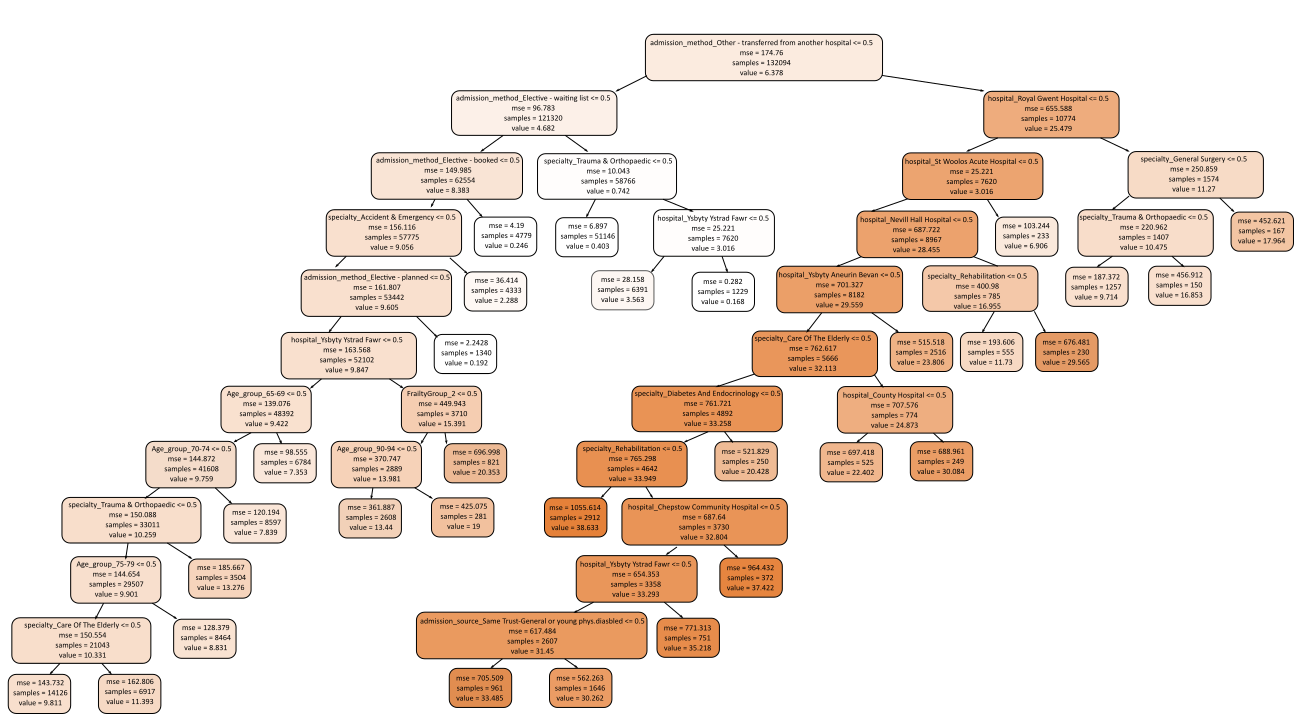
\includegraphics[scale=0.72]{Chapters/Chapter5/Figures/regressiontreevisual.png}
        \caption{Regression Tree Predicting Continuous LOS for Patients Within ABUHB}
        \label{fig:finalregtree}
    \end{figure}
\end{landscape}

\subsubsection{Classification Trees}
This section discusses the development and results of the classification trees, analysing grouped LOS into patients who are discharged on the same day as arrival and those who are admitted overnight. A total of ten variables will be used within the model, listed as follows:
\begin{multicols}{2}
    \begin{itemize}
        \item Admission Method
        \item Admission Source
        \item Age (Continuous and Grouped)
        \item Day
        \item Diagnosis
        \item Frailty (None, Continuous and Grouped)
        \item Hospital
        \item Month
        \item Number of Scans
        \item Specialty
    \end{itemize}
\end{multicols}

Unlike regression trees, month was included within the model as the accuracy score produced was greater than zero and could provide some benefit in being used within the model. 

Again, an 80\% training set and a 20\% test set was used to build and develop the model. Using the `DecisionTreeClassifier' algorithm within Python as discussed in Section \ref{sec:pythonclass}, the following parameters were selected for the model (Table \ref{tab:paramforclass}). The parameters `min\_samples\_leaf' and `max\_leaf\_nodes' will be investigated to determine the combination which yields the highest accuracy, precision and recall scores against the computational time.

\begin{table}[h!]
    \centering
    \begin{tabular}{lc}\toprule
      \textbf{Parameters}   & \textbf{DecisionTreeClassifier} \\\midrule
       criterion  & ``gini'' \\
       splitter & ``best'' \\
       max\_depth & None \\
       min\_samples\_split & 2 \\
       min\_weight\_fraction\_leaf & 0\\
       max\_features & None \\
       random\_state & None \\
       min\_impurity\_decrease & 0\\
       class\_weight & None \\
       ccp\_alpha &0\\ \bottomrule
    \end{tabular}
    \caption{Selected Parameters for `DecisionTreeClassifier'}
    \label{tab:paramforclass}
\end{table}

The accuracy scores for each of the six experiments range from 88.46\% to 89.89\%, a difference between 1.43\% (Tables \ref{tab:classtree1a} - \ref{tab:classtree6d}). This shows regardless of frailty and age classification, the difference is minimal between a range of different minimum samples per leaf and the maximum number of leaf nodes. The precision has a range of 4.41\%, from 84.75\% to 89.16\%. Comparing the accuracy to precision result, the highest values for each do not occur in the same `min\_samples\_leaf' and `max\_leaf\_nodes' combination. For example, comparing Table \ref{tab:classtree1a} with Table \ref{tab:classtree1b}, accuracy yielded the highest result with one minimum sample per leaf and 30 maximum leaf nodes. The highest precision results were recorded with 15 maximum leaf nodes, and either 400 or 500 minimum samples per leaf. The recall scores produced the largest result in the same combination as the accuracy scores (largest maximum leaf nodes and smallest minimum samples per leaf), however it produced the lowest score in the same location as the precision. Comparing the 400 minimum samples per leaf and 15 maximum leaf nodes suggests that FN $>$ FP. In terms of healthcare, this means patients are predicted to have short LOS's whereas in reality they have longer LOS's. Therefore, even though more costly as extra resources will be planned, it is beneficial to plan beds and not require them. This means the optimal solution should prioritise the recall score over the precision.

The optimum combination was selected to be one minimum sample per leaf with 30 maximum leaf nodes, using continuous age and continuous frailty (Tables \ref{tab:classtree2a} - \ref{tab:classtree2d}). This produced the highest accuracy and recall score, whilst also producing the lowest computational time out of the combination.

\begin{table}[h!]
\begin{subtable}{.49\linewidth}
    \centering\scalebox{0.55}{
    \begin{tabular}{ccx{1.4cm}x{1.4cm}x{1.4cm}x{1.4cm}x{1.4cm}x{1.4cm}}\toprule
    & \multicolumn{7}{c}{\textbf{min\_samples\_leaf}}\\
	&&\textbf{1} &	\textbf{100}	&\textbf{200}&	\textbf{300}&	\textbf{400}&	\textbf{500}\\\midrule
\parbox[t]{2mm}{\multirow{6}{*}{\rotatebox[origin=c]{90}{\textbf{max\_leaf\_nodes}}}} & \textbf{5}	& \ac{0.8846}	& \ac{0.8846} & \ac{0.8846}& \ac{0.8846} & \ac{0.8846} & \ac{0.8846} \\
&\textbf{10}	& \ac{0.8913}	&\ac{0.8913} &\ac{0.8913}&\ac{0.8913} & \ac{0.8913}&\ac{0.8913} \\
&\textbf{15}	& \ac{0.8950}	&\ac{0.8950} &\ac{0.8950}&\ac{0.8950} &\ac{0.8925}&\ac{0.8925} \\
&\textbf{20}	& \ac{0.8956}	&\ac{0.8956} &\ac{0.8950}&\ac{0.8950} & \ac{0.8936}&\ac{0.8936} \\
&\textbf{25}	& \ac{0.8977}	&\ac{0.8976} &\ac{0.8962}&\ac{0.8963} & \ac{0.8936}&\ac{0.8939} \\
&\textbf{30}	& \ac{0.8989}	&\ac{0.8987} &\ac{0.8968}&\ac{0.8968} & \ac{0.8939}&\ac{0.8937} \\\bottomrule

    \end{tabular}}
    \caption{Accuracy Score}
    \label{tab:classtree1a}
    \end{subtable}
\begin{subtable}{.5\linewidth}
  
    \centering\scalebox{0.55}{
    \begin{tabular}{ccx{1.4cm}x{1.4cm}x{1.4cm}x{1.4cm}x{1.4cm}x{1.4cm}}\toprule
    & \multicolumn{7}{c}{\textbf{min\_samples\_leaf}}\\
	&&\textbf{1} &	\textbf{100}	&\textbf{200}&	\textbf{300}&	\textbf{400}&	\textbf{500}\\\midrule
\parbox[t]{2mm}{\multirow{6}{*}{\rotatebox[origin=c]{90}{\textbf{max\_leaf\_nodes}}}} & \textbf{5}	& \pa{0.8475} & \pa{0.8475} & \pa{0.8475} & \pa{0.8475} & \pa{0.8475} & \pa{0.8475}\\
& \textbf{10} & \pa{0.8645} & \pa{0.8645} & \pa{0.8645} & \pa{0.8645} & \pa{0.8645} & \pa{0.8645} \\
& \textbf{15} & \pa{0.8643} & \pa{0.8643} & \pa{0.8643} & \pa{0.8643} & \pa{0.8916} & \pa{0.8916} \\
& \textbf{20} & \pa{0.8641} & \pa{0.8641} & \pa{0.8643} & \pa{0.8643} & \pa{0.8844} & \pa{0.8844} \\
& \textbf{25} & \pa{0.8637} & \pa{0.8617} & \pa{0.8598} & \pa{0.8594} & \pa{0.8844} & \pa{0.8804} \\
& \textbf{30} & \pa{0.8570} & \pa{0.8617} & \pa{0.8611} & \pa{0.8635} & \pa{0.8804} & \pa{0.8731} \\\bottomrule
    \end{tabular}}
    \caption{Precision Score}
    \label{tab:classtree1b}

\end{subtable}
\begin{subtable}{.49\linewidth}
    \centering\scalebox{0.55}{
    \begin{tabular}{ccx{1.4cm}x{1.4cm}x{1.4cm}x{1.4cm}x{1.4cm}x{1.4cm}}\toprule
    & \multicolumn{7}{c}{\textbf{min\_samples\_leaf}}\\
	&&\textbf{1} &	\textbf{100}	&\textbf{200}&	\textbf{300}&	\textbf{400}&	\textbf{500}\\\midrule
\parbox[t]{2mm}{\multirow{6}{*}{\rotatebox[origin=c]{90}{\textbf{max\_leaf\_nodes}}}} & \textbf{5}	& \re{0.8944}	& \re{0.8944} & \re{0.8944} & \re{0.8944} & \re{0.8944} & \re{0.8944} \\
&\textbf{10}	& \re{0.8941}	&\re{0.8941} &\re{0.8941}&\re{0.8941} & \re{0.8941}& \re{0.8941} \\
&\textbf{15}	& \re{0.8941}	&\re{0.9019} &\re{0.9019}&\re{0.9019} & \re{0.8755}& \re{0.8755} \\
&\textbf{20}	& \re{0.9033}	&\re{0.9033} &\re{0.9019}&\re{0.9019} & \re{0.8829}& \re{0.8829} \\
&\textbf{25}	& \re{0.9080}	&\re{0.9094} &\re{0.9081}&\re{0.9088} & \re{0.8829}& \re{0.8865} \\
&\textbf{30}	& \re{0.9163}	&\re{0.9117} &\re{0.9083}&\re{0.9061} & \re{0.8865}& \re{0.8919} \\\bottomrule

    \end{tabular}}
    \caption{Recall score}
    \label{tab:classtree1c}
    \end{subtable}
\begin{subtable}{.49\linewidth}

    
    \centering\scalebox{0.55}{
    \begin{tabular}{ccx{1.6cm}x{1.6cm}x{1.6cm}x{1.6cm}x{1.6cm}x{1.6cm}}\toprule
    & \multicolumn{7}{c}{\textbf{min\_samples\_leaf}}\\
	&&\textbf{1} &	\textbf{100}	&\textbf{200}&	\textbf{300}&	\textbf{400}&	\textbf{500}\\\midrule
\parbox[t]{2mm}{\multirow{6}{*}{\rotatebox[origin=c]{90}{\textbf{max\_leaf\_nodes}}}} & \textbf{5}	& \ti{9.1109} & \ti{8.3105} & \ti{8.2769} & \ti{8.7439} & \ti{13.1439} & \ti{10.0509}\\
& \textbf{10} & \ti{11.5346} & \ti{11.6610} & \ti{11.6360} & \ti{12.0482} & \ti{18.4817} & \ti{13.7823} \\
& \textbf{15} & \ti{14.8981} & \ti{13.3688} & \ti{14.2424} & \ti{14.0589} & \ti{16.0018} & \ti{17.7209} \\
& \textbf{20} & \ti{17.1809} & \ti{16.0233} & \ti{16.2691} & \ti{21.6318} & \ti{18.7793} & \ti{19.5191} \\
& \textbf{25} & \ti{17.3070} & \ti{17.6209} & \ti{17.1829} & \ti{22.8581} & \ti{21.2422} & \ti{20.4255} \\
& \textbf{30} & \ti{18.0397} & \ti{17.7756} & \ti{18.9454} & \ti{21.1663} & \ti{21.4531} & \ti{22.0665} \\\bottomrule

    \end{tabular}}
    \caption{Computational Time in Seconds (s)}
    \label{tab:classtree1d}

\end{subtable}


\label{tab:classtree1}
\caption{Classification Tree Accuracy, Precision, Recall and Computational Time Results - Continuous Age and No Frailty}
\end{table}




\begin{table}[h!]
\begin{subtable}{.49\linewidth}
    \centering\scalebox{0.55}{
    \begin{tabular}{ccx{1.4cm}x{1.4cm}x{1.4cm}x{1.4cm}x{1.4cm}x{1.4cm}}\toprule
    & \multicolumn{7}{c}{\textbf{min\_samples\_leaf}}\\
	&&\textbf{1} &	\textbf{100}	&\textbf{200}&	\textbf{300}&	\textbf{400}&	\textbf{500}\\\midrule
\parbox[t]{2mm}{\multirow{6}{*}{\rotatebox[origin=c]{90}{\textbf{max\_leaf\_nodes}}}} & \textbf{5}	& \ac{0.8846}	& \ac{0.8846} & \ac{0.8846}& \ac{0.8846} & \ac{0.8846} & \ac{0.8846} \\
&\textbf{10}	& \ac{0.8913}	&\ac{0.8913} &\ac{0.8913}&\ac{0.8913} & \ac{0.8913}&\ac{0.8913} \\
&\textbf{15}	& \ac{0.8950}	&\ac{0.8950} &\ac{0.8950}&\ac{0.8950} &\ac{0.8925}&\ac{0.8925} \\
&\textbf{20}	& \ac{0.8956}	&\ac{0.8956} &\ac{0.8950}&\ac{0.8950} & \ac{0.8925}&\ac{0.8925} \\
&\textbf{25}	& \ac{0.8977}	&\ac{0.8976} &\ac{0.8962}&\ac{0.8963} & \ac{0.8936}&\ac{0.8939} \\
&\textbf{30}	& \ac{0.8989}	&\ac{0.8987} &\ac{0.8968}&\ac{0.8968} & \ac{0.8941}&\ac{0.8939} \\\bottomrule

    \end{tabular}}
    \caption{Accuracy Score}
    \label{tab:classtree2a}
    \end{subtable}
\begin{subtable}{.5\linewidth}
  
    \centering\scalebox{0.55}{
    \begin{tabular}{ccx{1.4cm}x{1.4cm}x{1.4cm}x{1.4cm}x{1.4cm}x{1.4cm}}\toprule
    & \multicolumn{7}{c}{\textbf{min\_samples\_leaf}}\\
	&&\textbf{1} &	\textbf{100}	&\textbf{200}&	\textbf{300}&	\textbf{400}&	\textbf{500}\\\midrule
\parbox[t]{2mm}{\multirow{6}{*}{\rotatebox[origin=c]{90}{\textbf{max\_leaf\_nodes}}}} & \textbf{5}	& \pa{0.8475} & \pa{0.8475} & \pa{0.8475} & \pa{0.8475} & \pa{0.8475} & \pa{0.8475}\\
& \textbf{10} & \pa{0.8645} & \pa{0.8645} & \pa{0.8645} & \pa{0.8645} & \pa{0.8645} & \pa{0.8645} \\
& \textbf{15} & \pa{0.8643} & \pa{0.8643} & \pa{0.8643} & \pa{0.8643} & \pa{0.8916} & \pa{0.8916} \\
& \textbf{20} & \pa{0.8641} & \pa{0.8641} & \pa{0.8643} & \pa{0.8643} & \pa{0.8916} & \pa{0.8916} \\
& \textbf{25} & \pa{0.8637} & \pa{0.8617} & \pa{0.8598} & \pa{0.8594} & \pa{0.8844} & \pa{0.8804} \\
& \textbf{30} & \pa{0.8570} & \pa{0.8617} & \pa{0.8611} & \pa{0.8635} & \pa{0.8812} & \pa{0.8804} \\\bottomrule
    \end{tabular}}
    \caption{Precision Score}
    \label{tab:classtree2b}

\end{subtable}
\begin{subtable}{.49\linewidth}
    \centering\scalebox{0.55}{
    \begin{tabular}{ccx{1.4cm}x{1.4cm}x{1.4cm}x{1.4cm}x{1.4cm}x{1.4cm}}\toprule
    & \multicolumn{7}{c}{\textbf{min\_samples\_leaf}}\\
	&&\textbf{1} &	\textbf{100}	&\textbf{200}&	\textbf{300}&	\textbf{400}&	\textbf{500}\\\midrule
\parbox[t]{2mm}{\multirow{6}{*}{\rotatebox[origin=c]{90}{\textbf{max\_leaf\_nodes}}}} & \textbf{5}	& \re{0.8944}	& \re{0.8944} & \re{0.8944} & \re{0.8944} & \re{0.8944} & \re{0.8944} \\
&\textbf{10}	& \re{0.8941}	&\re{0.8941} &\re{0.8941}&\re{0.8941} & \re{0.8941}& \re{0.8941} \\
&\textbf{15}	& \re{0.9019}	&\re{0.9019} &\re{0.9019}&\re{0.9019} & \re{0.8755}& \re{0.8755} \\
&\textbf{20}	& \re{0.9033}	&\re{0.9033} &\re{0.9019}&\re{0.9019} & \re{0.8755}& \re{0.8755} \\
&\textbf{25}	& \re{0.9080}	&\re{0.9094} &\re{0.9081}&\re{0.9088} & \re{0.8829}& \re{0.8865} \\
&\textbf{30}	& \re{0.9163}	&\re{0.9117} &\re{0.9083}&\re{0.9061} & \re{0.8863}& \re{0.8865} \\\bottomrule

    \end{tabular}}
    \caption{Recall score}
    \label{tab:classtree2c}
    \end{subtable}
\begin{subtable}{.49\linewidth}

    
    \centering\scalebox{0.55}{
    \begin{tabular}{ccx{1.6cm}x{1.6cm}x{1.6cm}x{1.6cm}x{1.6cm}x{1.6cm}}\toprule
    & \multicolumn{7}{c}{\textbf{min\_samples\_leaf}}\\
	&&\textbf{1} &	\textbf{100}	&\textbf{200}&	\textbf{300}&	\textbf{400}&	\textbf{500}\\\midrule
\parbox[t]{2mm}{\multirow{6}{*}{\rotatebox[origin=c]{90}{\textbf{max\_leaf\_nodes}}}} & \textbf{5}	& \ti{7.8660} & \ti{7.8724} & \ti{7.9036} & \ti{10.9756} & \ti{7.9045} & \ti{8.0315}\\
& \textbf{10} & \ti{10.7175} & \ti{11.0817} & \ti{10.9410} & \ti{13.6632} & \ti{11.7000} & \ti{11.1358} \\
& \textbf{15} & \ti{12.9169} & \ti{12.8437} & \ti{12.6717} & \ti{16.5188} & \ti{13.4148} & \ti{12.7473} \\
& \textbf{20} & \ti{15.1352} & \ti{14.7659} & \ti{14.7613} & \ti{16.1299} & \ti{15.6667} & \ti{14.9961} \\
& \textbf{25} & \ti{16.1773} & \ti{15.0654} & \ti{15.7308} & \ti{16.7057} & \ti{18.3250} & \ti{16.5215}  \\
& \textbf{30} & \ti{16.7448} & \ti{16.9692} & \ti{17.1850} & \ti{17.7688} & \ti{16.7887} & \ti{17.6103} \\\bottomrule

    \end{tabular}}
    \caption{Computational Time in Seconds (s)}
    \label{tab:classtree2d}
\end{subtable}
\label{tab:classtree2}
\caption{Classification Tree Accuracy, Precision, Recall and Computational Time Results - Continuous Age and Continuous Frailty}
\end{table}



\begin{table}[h!]
\begin{subtable}{.49\linewidth}
    \centering\scalebox{0.55}{
    \begin{tabular}{ccx{1.4cm}x{1.4cm}x{1.4cm}x{1.4cm}x{1.4cm}x{1.4cm}}\toprule
    & \multicolumn{7}{c}{\textbf{min\_samples\_leaf}}\\
	&&\textbf{1} &	\textbf{100}	&\textbf{200}&	\textbf{300}&	\textbf{400}&	\textbf{500}\\\midrule
\parbox[t]{2mm}{\multirow{6}{*}{\rotatebox[origin=c]{90}{\textbf{max\_leaf\_nodes}}}} & \textbf{5}	& \ac{0.8846}	& \ac{0.8846} & \ac{0.8846}& \ac{0.8846} & \ac{0.8846} & \ac{0.8846} \\
&\textbf{10}	& \ac{0.8913}	&\ac{0.8913} &\ac{0.8913}&\ac{0.8913} & \ac{0.8913}&\ac{0.8913} \\
&\textbf{15}	& \ac{0.8950}	&\ac{0.8950} &\ac{0.8950}&\ac{0.8950} &\ac{0.8925}&\ac{0.8925} \\
&\textbf{20}	& \ac{0.8956}	&\ac{0.8956} &\ac{0.8950}&\ac{0.8950} & \ac{0.8925}&\ac{0.8925} \\
&\textbf{25}	& \ac{0.8977}	&\ac{0.8976} &\ac{0.8962}&\ac{0.8963} & \ac{0.8936}&\ac{0.8936} \\
&\textbf{30}	& \ac{0.8989}	&\ac{0.8987} &\ac{0.8968}&\ac{0.8968} & \ac{0.8941}&\ac{0.8941} \\\bottomrule

    \end{tabular}}
    \caption{Accuracy Score}
    \label{tab:classtree3a}
    \end{subtable}
\begin{subtable}{.5\linewidth}
  
    \centering\scalebox{0.55}{
    \begin{tabular}{ccx{1.4cm}x{1.4cm}x{1.4cm}x{1.4cm}x{1.4cm}x{1.4cm}}\toprule
    & \multicolumn{7}{c}{\textbf{min\_samples\_leaf}}\\
	&&\textbf{1} &	\textbf{100}	&\textbf{200}&	\textbf{300}&	\textbf{400}&	\textbf{500}\\\midrule
\parbox[t]{2mm}{\multirow{6}{*}{\rotatebox[origin=c]{90}{\textbf{max\_leaf\_nodes}}}} & \textbf{5}	& \pa{0.8475} & \pa{0.8475} & \pa{0.8475} & \pa{0.8475} & \pa{0.8475} & \pa{0.8475}\\
& \textbf{10} & \pa{0.8645} & \pa{0.8645} & \pa{0.8645} & \pa{0.8645} & \pa{0.8645} & \pa{0.8645} \\
& \textbf{15} & \pa{0.8643} & \pa{0.8643} & \pa{0.8643} & \pa{0.8643} & \pa{0.8916} & \pa{0.8916} \\
& \textbf{20} & \pa{0.8641} & \pa{0.8641} & \pa{0.8643} & \pa{0.8643} & \pa{0.8916} & \pa{0.8916} \\
& \textbf{25} & \pa{0.8637} & \pa{0.8617} & \pa{0.8598} & \pa{0.8594} & \pa{0.8844} & \pa{0.8844} \\
& \textbf{30} & \pa{0.8570} & \pa{0.8617} & \pa{0.8611} & \pa{0.8635} & \pa{0.8810} & \pa{0.8844} \\\bottomrule
    \end{tabular}}
    \caption{Precision Score}
    \label{tab:classtree3b}

\end{subtable}
\begin{subtable}{.49\linewidth}
    \centering\scalebox{0.55}{
    \begin{tabular}{ccx{1.4cm}x{1.4cm}x{1.4cm}x{1.4cm}x{1.4cm}x{1.4cm}}\toprule
    & \multicolumn{7}{c}{\textbf{min\_samples\_leaf}}\\
	&&\textbf{1} &	\textbf{100}	&\textbf{200}&	\textbf{300}&	\textbf{400}&	\textbf{500}\\\midrule
\parbox[t]{2mm}{\multirow{6}{*}{\rotatebox[origin=c]{90}{\textbf{max\_leaf\_nodes}}}} & \textbf{5}	& \re{0.8944}	& \re{0.8944} & \re{0.8944} & \re{0.8944} & \re{0.8944} & \re{0.8944} \\
&\textbf{10}	& \re{0.8941}	&\re{0.8941} &\re{0.8941}&\re{0.8941} & \re{0.8941}& \re{0.8941} \\
&\textbf{15}	& \re{0.9019}	&\re{0.9019} &\re{0.9019}&\re{0.9019} & \re{0.8755}& \re{0.8755} \\
&\textbf{20}	& \re{0.9033}	&\re{0.9033} &\re{0.9019}&\re{0.9019} & \re{0.8755}& \re{0.8755} \\
&\textbf{25}	& \re{0.9080}	&\re{0.9094} &\re{0.9081}&\re{0.9088} & \re{0.8829}& \re{0.8829} \\
&\textbf{30}	& \re{0.9163}	&\re{0.9117} &\re{0.9083}&\re{0.9061} & \re{0.8865}& \re{0.8829} \\\bottomrule

    \end{tabular}}
    \caption{Recall score}
    \label{tab:classtree3c}
    \end{subtable}
\begin{subtable}{.49\linewidth}

    
    \centering\scalebox{0.55}{
    \begin{tabular}{ccx{1.6cm}x{1.6cm}x{1.6cm}x{1.6cm}x{1.6cm}x{1.6cm}}\toprule
    & \multicolumn{7}{c}{\textbf{min\_samples\_leaf}}\\
	&&\textbf{1} &	\textbf{100}	&\textbf{200}&	\textbf{300}&	\textbf{400}&	\textbf{500}\\\midrule
\parbox[t]{2mm}{\multirow{6}{*}{\rotatebox[origin=c]{90}{\textbf{max\_leaf\_nodes}}}} & \textbf{5}	& \ti{8.3217} & \ti{8.5695} & \ti{8.8101} & \ti{8.8153} & \ti{11.3366} & \ti{25.3592}\\
& \textbf{10} & \ti{11.3205} & \ti{11.6050} & \ti{11.8029} & \ti{12.3844} & \ti{14.7207} & \ti{17.2309} \\
& \textbf{15} & \ti{13.5908} & \ti{13.5596} & \ti{13.6742} & \ti{13.7826} & \ti{20.0681} & \ti{16.4461} \\
& \textbf{20} & \ti{15.5900} & \ti{15.6141} & \ti{15.9532} & \ti{15.9093} & \ti{20.6382} & \ti{20.5908} \\
& \textbf{25} & \ti{16.5625} & \ti{16.1451} & \ti{16.9353} & \ti{17.2625} & \ti{19.2398} & \ti{19.6446}  \\
& \textbf{30} & \ti{17.8176} & \ti{17.5732} & \ti{18.1772} & \ti{19.2464} & \ti{25.3592} & \ti{22.3077} \\\bottomrule

    \end{tabular}}
    \caption{Computational Time in Seconds (s)}
    \label{tab:classtree3d}

\end{subtable}

\label{tab:classtree3}
\caption{Classification Tree Accuracy, Precision, Recall and Computational Time Results - Continuous Age and Grouped Frailty}
\end{table}



\begin{table}[h!]
\begin{subtable}{.49\linewidth}
    \centering\scalebox{0.55}{
    \begin{tabular}{ccx{1.4cm}x{1.4cm}x{1.4cm}x{1.4cm}x{1.4cm}x{1.4cm}}\toprule
    & \multicolumn{7}{c}{\textbf{min\_samples\_leaf}}\\
	&&\textbf{1} &	\textbf{100}	&\textbf{200}&	\textbf{300}&	\textbf{400}&	\textbf{500}\\\midrule
\parbox[t]{2mm}{\multirow{6}{*}{\rotatebox[origin=c]{90}{\textbf{max\_leaf\_nodes}}}} & \textbf{5}	& \ac{0.8846}	& \ac{0.8846} & \ac{0.8846}& \ac{0.8846} & \ac{0.8846} & \ac{0.8846} \\
&\textbf{10}	& \ac{0.8913}	&\ac{0.8913} &\ac{0.8913}&\ac{0.8913} & \ac{0.8913}&\ac{0.8913} \\
&\textbf{15}	& \ac{0.8950}	&\ac{0.8950} &\ac{0.8950}&\ac{0.8950} &\ac{0.8925}&\ac{0.8925} \\
&\textbf{20}	& \ac{0.8956}	&\ac{0.8956} &\ac{0.8956}&\ac{0.8956} & \ac{0.8936}&\ac{0.8939} \\
&\textbf{25}	& \ac{0.8977}	&\ac{0.8976} &\ac{0.8962}&\ac{0.8963} & \ac{0.8936}&\ac{0.8939} \\
&\textbf{30}	& \ac{0.8989}	&\ac{0.8987} &\ac{0.8968}&\ac{0.8968} & \ac{0.8939}&\ac{0.8937} \\\bottomrule

    \end{tabular}}
    \caption{Accuracy Score}
    \label{tab:classtree4a}
    \end{subtable}
\begin{subtable}{.5\linewidth}
  
    \centering\scalebox{0.55}{
    \begin{tabular}{ccx{1.4cm}x{1.4cm}x{1.4cm}x{1.4cm}x{1.4cm}x{1.4cm}}\toprule
    & \multicolumn{7}{c}{\textbf{min\_samples\_leaf}}\\
	&&\textbf{1} &	\textbf{100}	&\textbf{200}&	\textbf{300}&	\textbf{400}&	\textbf{500}\\\midrule
\parbox[t]{2mm}{\multirow{6}{*}{\rotatebox[origin=c]{90}{\textbf{max\_leaf\_nodes}}}} & \textbf{5}	& \pa{0.8475} & \pa{0.8475} & \pa{0.8475} & \pa{0.8475} & \pa{0.8475} & \pa{0.8475}\\
& \textbf{10} & \pa{0.8645} & \pa{0.8645} & \pa{0.8645} & \pa{0.8645} & \pa{0.8645} & \pa{0.8645} \\
& \textbf{15} & \pa{0.8643} & \pa{0.8643} & \pa{0.8643} & \pa{0.8643} & \pa{0.8916} & \pa{0.8916} \\
& \textbf{20} & \pa{0.8641} & \pa{0.8641} & \pa{0.8643} & \pa{0.8643} & \pa{0.8944} & \pa{0.8944} \\
& \textbf{25} & \pa{0.8637} & \pa{0.8617} & \pa{0.8598} & \pa{0.8594} & \pa{0.8844} & \pa{0.8804} \\
& \textbf{30} & \pa{0.8570} & \pa{0.8617} & \pa{0.8611} & \pa{0.8635} & \pa{0.8804} & \pa{0.8731} \\\bottomrule
    \end{tabular}}
    \caption{Precision Score}
    \label{tab:classtree4b}

\end{subtable}
\begin{subtable}{.49\linewidth}
    \centering\scalebox{0.55}{
    \begin{tabular}{ccx{1.4cm}x{1.4cm}x{1.4cm}x{1.4cm}x{1.4cm}x{1.4cm}}\toprule
    & \multicolumn{7}{c}{\textbf{min\_samples\_leaf}}\\
	&&\textbf{1} &	\textbf{100}	&\textbf{200}&	\textbf{300}&	\textbf{400}&	\textbf{500}\\\midrule
\parbox[t]{2mm}{\multirow{6}{*}{\rotatebox[origin=c]{90}{\textbf{max\_leaf\_nodes}}}} & \textbf{5}	& \re{0.8944}	& \re{0.8944} & \re{0.8944} & \re{0.8944} & \re{0.8944} & \re{0.8944} \\
&\textbf{10}	& \re{0.8941}	&\re{0.8941} &\re{0.8941}&\re{0.8941} & \re{0.8941}& \re{0.8941} \\
&\textbf{15}	& \re{0.9019}	&\re{0.9019} &\re{0.9019}&\re{0.9019} & \re{0.8755}& \re{0.8755} \\
&\textbf{20}	& \re{0.9033}	&\re{0.9033} &\re{0.9019}&\re{0.9019} & \re{0.8829}& \re{0.8829} \\
&\textbf{25}	& \re{0.9080}	&\re{0.9094} &\re{0.9081}&\re{0.9088} & \re{0.8829}& \re{0.8865} \\
&\textbf{30}	& \re{0.9163}	&\re{0.9117} &\re{0.9083}&\re{0.9061} & \re{0.8865}& \re{0.8819} \\\bottomrule

    \end{tabular}}
    \caption{Recall score}
    \label{tab:classtree4c}
    \end{subtable}
\begin{subtable}{.49\linewidth}

    
    \centering\scalebox{0.55}{
    \begin{tabular}{ccx{1.6cm}x{1.6cm}x{1.6cm}x{1.6cm}x{1.6cm}x{1.6cm}}\toprule
    & \multicolumn{7}{c}{\textbf{min\_samples\_leaf}}\\
	&&\textbf{1} &	\textbf{100}	&\textbf{200}&	\textbf{300}&	\textbf{400}&	\textbf{500}\\\midrule
\parbox[t]{2mm}{\multirow{6}{*}{\rotatebox[origin=c]{90}{\textbf{max\_leaf\_nodes}}}} & \textbf{5}	& \ti{9.0003} & \ti{9.1338} & \ti{8.0463} & \ti{7.9693} & \ti{8.0229} & \ti{7.9960}\\
& \textbf{10} & \ti{11.8935} & \ti{12.6970} & \ti{11.2224} & \ti{11.1074} & \ti{11.3092} & \ti{11.2887} \\
& \textbf{15} & \ti{13.8198} & \ti{13.0589} & \ti{13.0067} & \ti{13.5755} & \ti{13.3384} & \ti{13.1068} \\
& \textbf{20} & \ti{16.3988} & \ti{15.6034} & \ti{14.9843} & \ti{15.0497} & \ti{15.4588} & \ti{15.3504} \\
& \textbf{25} & \ti{20.8890} & \ti{15.9613} & \ti{16.0429} & \ti{17.0717} & \ti{16.3030} & \ti{16.8512}  \\
& \textbf{30} & \ti{24.0505} & \ti{18.3618} & \ti{17.5238} & \ti{17.6762} & \ti{17.7605} & \ti{17.3051} \\\bottomrule

    \end{tabular}}
    \caption{Computational Time in Seconds (s)}
    \label{tab:classtree4d}

\end{subtable}

\label{tab:classtree4}
\caption{Classification Tree Accuracy, Precision, Recall and Computational Time Results - Grouped Age and No Frailty}
\end{table}


\begin{table}[h!]
\begin{subtable}{.49\linewidth}
    \centering\scalebox{0.55}{
    \begin{tabular}{ccx{1.4cm}x{1.4cm}x{1.4cm}x{1.4cm}x{1.4cm}x{1.4cm}}\toprule
    & \multicolumn{7}{c}{\textbf{min\_samples\_leaf}}\\
	&&\textbf{1} &	\textbf{100}	&\textbf{200}&	\textbf{300}&	\textbf{400}&	\textbf{500}\\\midrule
\parbox[t]{2mm}{\multirow{6}{*}{\rotatebox[origin=c]{90}{\textbf{max\_leaf\_nodes}}}} & \textbf{5}	& \ac{0.8846}	& \ac{0.8846} & \ac{0.8846}& \ac{0.8846} & \ac{0.8846} & \ac{0.8846} \\
&\textbf{10}	& \ac{0.8913}	&\ac{0.8913} &\ac{0.8913}&\ac{0.8913} & \ac{0.8913}&\ac{0.8913} \\
&\textbf{15}	& \ac{0.8950}	&\ac{0.8950} &\ac{0.8950}&\ac{0.8950} &\ac{0.8925}&\ac{0.8925} \\
&\textbf{20}	& \ac{0.8956}	&\ac{0.8956} &\ac{0.8950}&\ac{0.8950} & \ac{0.8925}&\ac{0.8925} \\
&\textbf{25}	& \ac{0.8977}	&\ac{0.8976} &\ac{0.8962}&\ac{0.8963} & \ac{0.8936}&\ac{0.8939} \\
&\textbf{30}	& \ac{0.8989}	&\ac{0.8987} &\ac{0.8968}&\ac{0.8968} & \ac{0.8941}&\ac{0.8939} \\\bottomrule

    \end{tabular}}
    \caption{Accuracy Score}
    \label{tab:classtree5a}
    \end{subtable}
\begin{subtable}{.5\linewidth}
  
    \centering\scalebox{0.55}{
    \begin{tabular}{ccx{1.4cm}x{1.4cm}x{1.4cm}x{1.4cm}x{1.4cm}x{1.4cm}}\toprule
    & \multicolumn{7}{c}{\textbf{min\_samples\_leaf}}\\
	&&\textbf{1} &	\textbf{100}	&\textbf{200}&	\textbf{300}&	\textbf{400}&	\textbf{500}\\\midrule
\parbox[t]{2mm}{\multirow{6}{*}{\rotatebox[origin=c]{90}{\textbf{max\_leaf\_nodes}}}} & \textbf{5}	& \pa{0.8475} & \pa{0.8475} & \pa{0.8475} & \pa{0.8475} & \pa{0.8475} & \pa{0.8475}\\
& \textbf{10} & \pa{0.8645} & \pa{0.8645} & \pa{0.8645} & \pa{0.8645} & \pa{0.8645} & \pa{0.8645} \\
& \textbf{15} & \pa{0.8643} & \pa{0.8643} & \pa{0.8643} & \pa{0.8643} & \pa{0.8916} & \pa{0.8916} \\
& \textbf{20} & \pa{0.8641} & \pa{0.8641} & \pa{0.8643} & \pa{0.8643} & \pa{0.8916} & \pa{0.8916} \\
& \textbf{25} & \pa{0.8637} & \pa{0.8617} & \pa{0.8598} & \pa{0.8594} & \pa{0.8844} & \pa{0.8804} \\
& \textbf{30} & \pa{0.8570} & \pa{0.8617} & \pa{0.8611} & \pa{0.8635} & \pa{0.8812} & \pa{0.8804} \\\bottomrule
    \end{tabular}}
    \caption{Precision Score}
    \label{tab:classtree5b}

\end{subtable}
\begin{subtable}{.49\linewidth}
    \centering\scalebox{0.55}{
    \begin{tabular}{ccx{1.4cm}x{1.4cm}x{1.4cm}x{1.4cm}x{1.4cm}x{1.4cm}}\toprule
    & \multicolumn{7}{c}{\textbf{min\_samples\_leaf}}\\
	&&\textbf{1} &	\textbf{100}	&\textbf{200}&	\textbf{300}&	\textbf{400}&	\textbf{500}\\\midrule
\parbox[t]{2mm}{\multirow{6}{*}{\rotatebox[origin=c]{90}{\textbf{max\_leaf\_nodes}}}} & \textbf{5}	& \re{0.8944}	& \re{0.8944} & \re{0.8944} & \re{0.8944} & \re{0.8944} & \re{0.8944} \\
&\textbf{10}	& \re{0.8941}	&\re{0.8941} &\re{0.8941}&\re{0.8941} & \re{0.8941}& \re{0.8941} \\
&\textbf{15}	& \re{0.9019}	&\re{0.9019} &\re{0.9019}&\re{0.9019} & \re{0.8755}& \re{0.8755} \\
&\textbf{20}	& \re{0.9033}	&\re{0.9033} &\re{0.9019}&\re{0.9019} & \re{0.8755}& \re{0.8755} \\
&\textbf{25}	& \re{0.9080}	&\re{0.9094} &\re{0.9081}&\re{0.9088} & \re{0.8829}& \re{0.8865} \\
&\textbf{30}	& \re{0.9163}	&\re{0.9117} &\re{0.9083}&\re{0.9061} & \re{0.8863}& \re{0.8865} \\\bottomrule

    \end{tabular}}
    \caption{Recall score}
    \label{tab:classtree5c}
    \end{subtable}
\begin{subtable}{.49\linewidth}

    
    \centering\scalebox{0.55}{
    \begin{tabular}{ccx{1.6cm}x{1.6cm}x{1.6cm}x{1.6cm}x{1.6cm}x{1.6cm}}\toprule
    & \multicolumn{7}{c}{\textbf{min\_samples\_leaf}}\\
	&&\textbf{1} &	\textbf{100}	&\textbf{200}&	\textbf{300}&	\textbf{400}&	\textbf{500}\\\midrule
\parbox[t]{2mm}{\multirow{6}{*}{\rotatebox[origin=c]{90}{\textbf{max\_leaf\_nodes}}}} & \textbf{5}	& \ti{9.0269} & \ti{8.7352} & \ti{9.0878} & \ti{8.5125} & \ti{8.1122} & \ti{8.6958}\\
& \textbf{10} & \ti{12.0635} & \ti{12.2949} & \ti{12.1766} & \ti{11.5033} & \ti{12.1410} & \ti{12.7141} \\
& \textbf{15} & \ti{13.8758} & \ti{14.2554} & \ti{14.4314} & \ti{13.3940} & \ti{14.7385} & \ti{15.0438} \\
& \textbf{20} & \ti{16.0829} & \ti{15.9826} & \ti{15.1769} & \ti{15.3548} & \ti{17.0093} & \ti{17.0980} \\
& \textbf{25} & \ti{16.9550} & \ti{17.4665} & \ti{16.3701} & \ti{16.8606} & \ti{18.1321} & \ti{20.0174}  \\
& \textbf{30} & \ti{18.0005} & \ti{18.0719} & \ti{18.6015} & \ti{18.0826} & \ti{18.6726} & \ti{19.3604} \\\bottomrule

    \end{tabular}}
    \caption{Computational Time in Seconds (s)}
    \label{tab:classtree5d}

\end{subtable}

\label{tab:classtree5}
\caption{Classification Tree Accuracy, Precision, Recall and Computational Time Results - Grouped Age and Continuous Frailty}
\end{table}


\begin{table}[h!]
\begin{subtable}{.49\linewidth}
    \centering\scalebox{0.55}{
    \begin{tabular}{ccx{1.4cm}x{1.4cm}x{1.4cm}x{1.4cm}x{1.4cm}x{1.4cm}}\toprule
    & \multicolumn{7}{c}{\textbf{min\_samples\_leaf}}\\
	&&\textbf{1} &	\textbf{100}	&\textbf{200}&	\textbf{300}&	\textbf{400}&	\textbf{500}\\\midrule
\parbox[t]{2mm}{\multirow{6}{*}{\rotatebox[origin=c]{90}{\textbf{max\_leaf\_nodes}}}} & \textbf{5}	& \ac{0.8846}	& \ac{0.8846} & \ac{0.8846}& \ac{0.8846} & \ac{0.8846} & \ac{0.8846} \\
&\textbf{10}	& \ac{0.8913}	&\ac{0.8913} &\ac{0.8913}&\ac{0.8913} & \ac{0.8913}&\ac{0.8913} \\
&\textbf{15}	& \ac{0.8950}	&\ac{0.8950} &\ac{0.8950}&\ac{0.8950} &\ac{0.8925}&\ac{0.8925} \\
&\textbf{20}	& \ac{0.8956}	&\ac{0.8956} &\ac{0.8950}&\ac{0.8950} & \ac{0.8925}&\ac{0.8925} \\
&\textbf{25}	& \ac{0.8977}	&\ac{0.8976} &\ac{0.8962}&\ac{0.8963} & \ac{0.8936}&\ac{0.8936} \\
&\textbf{30}	& \ac{0.8989}	&\ac{0.8987} &\ac{0.8968}&\ac{0.8968} & \ac{0.8941}&\ac{0.8936} \\\bottomrule

    \end{tabular}}
    \caption{Accuracy Score}
    \label{tab:classtree6a}
    \end{subtable}
\begin{subtable}{.5\linewidth}
  
    \centering\scalebox{0.55}{
    \begin{tabular}{ccx{1.4cm}x{1.4cm}x{1.4cm}x{1.4cm}x{1.4cm}x{1.4cm}}\toprule
    & \multicolumn{7}{c}{\textbf{min\_samples\_leaf}}\\
	&&\textbf{1} &	\textbf{100}	&\textbf{200}&	\textbf{300}&	\textbf{400}&	\textbf{500}\\\midrule
\parbox[t]{2mm}{\multirow{6}{*}{\rotatebox[origin=c]{90}{\textbf{max\_leaf\_nodes}}}} & \textbf{5}	& \pa{0.8475} & \pa{0.8475} & \pa{0.8475} & \pa{0.8475} & \pa{0.8475} & \pa{0.8475}\\
& \textbf{10} & \pa{0.8645} & \pa{0.8645} & \pa{0.8645} & \pa{0.8645} & \pa{0.8645} & \pa{0.8645} \\
& \textbf{15} & \pa{0.8643} & \pa{0.8643} & \pa{0.8643} & \pa{0.8643} & \pa{0.8916} & \pa{0.8916} \\
& \textbf{20} & \pa{0.8641} & \pa{0.8641} & \pa{0.8643} & \pa{0.8643} & \pa{0.8916} & \pa{0.8916} \\
& \textbf{25} & \pa{0.8637} & \pa{0.8617} & \pa{0.8598} & \pa{0.8594} & \pa{0.8844} & \pa{0.8844} \\
& \textbf{30} & \pa{0.8570} & \pa{0.8617} & \pa{0.8611} & \pa{0.8635} & \pa{0.8810} & \pa{0.8844} \\\bottomrule
    \end{tabular}}
    \caption{Precision Score}
    \label{tab:classtree6b}

\end{subtable}
\begin{subtable}{.49\linewidth}
    \centering\scalebox{0.55}{
    \begin{tabular}{ccx{1.4cm}x{1.4cm}x{1.4cm}x{1.4cm}x{1.4cm}x{1.4cm}}\toprule
    & \multicolumn{7}{c}{\textbf{min\_samples\_leaf}}\\
	&&\textbf{1} &	\textbf{100}	&\textbf{200}&	\textbf{300}&	\textbf{400}&	\textbf{500}\\\midrule
\parbox[t]{2mm}{\multirow{6}{*}{\rotatebox[origin=c]{90}{\textbf{max\_leaf\_nodes}}}} & \textbf{5}	& \re{0.8944}	& \re{0.8944} & \re{0.8944} & \re{0.8944} & \re{0.8944} & \re{0.8944} \\
&\textbf{10}	& \re{0.8941}	&\re{0.8941} &\re{0.8941}&\re{0.8941} & \re{0.8941}& \re{0.8941} \\
&\textbf{15}	& \re{0.9019}	&\re{0.9019} &\re{0.9019}&\re{0.9019} & \re{0.8755}& \re{0.8755} \\
&\textbf{20}	& \re{0.9033}	&\re{0.9033} &\re{0.9019}&\re{0.9019} & \re{0.8755}& \re{0.8755} \\
&\textbf{25}	& \re{0.9080}	&\re{0.9094} &\re{0.9081}&\re{0.9088} & \re{0.8829}& \re{0.8829} \\
&\textbf{30}	& \re{0.9163}	&\re{0.9117} &\re{0.9083}&\re{0.9061} & \re{0.8865}& \re{0.8829} \\\bottomrule

    \end{tabular}}
    \caption{Recall score}
    \label{tab:classtree6c}
    \end{subtable}
\begin{subtable}{.49\linewidth}

    
    \centering\scalebox{0.55}{
    \begin{tabular}{ccx{1.6cm}x{1.6cm}x{1.6cm}x{1.6cm}x{1.6cm}x{1.6cm}}\toprule
    & \multicolumn{7}{c}{\textbf{min\_samples\_leaf}}\\
	&&\textbf{1} &	\textbf{100}	&\textbf{200}&	\textbf{300}&	\textbf{400}&	\textbf{500}\\\midrule
\parbox[t]{2mm}{\multirow{6}{*}{\rotatebox[origin=c]{90}{\textbf{max\_leaf\_nodes}}}} & \textbf{5}	& \ti{8.9117} & \ti{8.9096} & \ti{10.8248} & \ti{9.9785} & \ti{8.8351} & \ti{10.1257}\\
& \textbf{10} & \ti{12.1086} & \ti{12.1666} & \ti{13.6021} & \ti{14.9230} & \ti{12.3419} & \ti{12.3234} \\
& \textbf{15} & \ti{14.0532} & \ti{17.2649} & \ti{16.1410} & \ti{16.0983} & \ti{14.5993} & \ti{13.8329} \\
& \textbf{20} & \ti{16.5178} & \ti{17.3444} & \ti{21.1871} & \ti{17.1917} & \ti{17.0247} & \ti{15.6259} \\
& \textbf{25} & \ti{17.5062} & \ti{19.6158} & \ti{19.7483} & \ti{17.1917} & \ti{17.5036} & \ti{16.7736}  \\
& \textbf{30} & \ti{17.9821} & \ti{20.0913} & \ti{19.3814} & \ti{19.3519} & \ti{18.2937} & \ti{17.5289} \\\bottomrule

    \end{tabular}}
    \caption{Computational Time in Seconds (s)}
    \label{tab:classtree6d}

\end{subtable}

\label{tab:classtree5}
\caption{Classification Tree Accuracy, Precision, Recall and Computational Time Results - Grouped Age and Grouped Frailty}
\end{table}


Figure \ref{fig:finalclasstree} displays the classification tree visualisation with an accuracy score of 89.89\%, a precision score of 85.70\% and a recall score of 91.63\%. The tree shows the most important factor to determine whether a patient will be admitted overnight is the `admission\_method\_elective - waiting list'. If a patient was admitted via this method, then they are more likely to be discharged on the same day. The class displayed on the node represents the highest quantity of patients. The colours of the node symbolise the weighting within the group, with the darkest orange representing discharge on the same day ($<$1) and the darkest blue representing admittance overnight ($\geq$1). There are 16 leaf nodes representing the $\geq1$ class, with one node generating a gini of zero, and therefore is a perfect classification.

The model produced 30 leaf nodes, displaying the class of patient, the majority fall into. The user is then able to analyse the individual results within the nodes to determine the average LOS's. This is also beneficial to determine where targets of being discharged on the same day of admission is not being met, for example surgical cases. It also displays influencing factors in LOS. For example, a patient who are admitted through the elective waiting list to the specialty gynaecology, will have their LOS dependent on the day they are admitted. If they are admitted on a Monday, they fall into the ``$\geq1$'' class, otherwise they fall into the ``$<1$'' class. This can be used to help practitioners plan elective admission and when they should be admitted in order to reduce unexpected and prolonged LOS's.


\begin{landscape}
    \begin{figure}
        \centering
        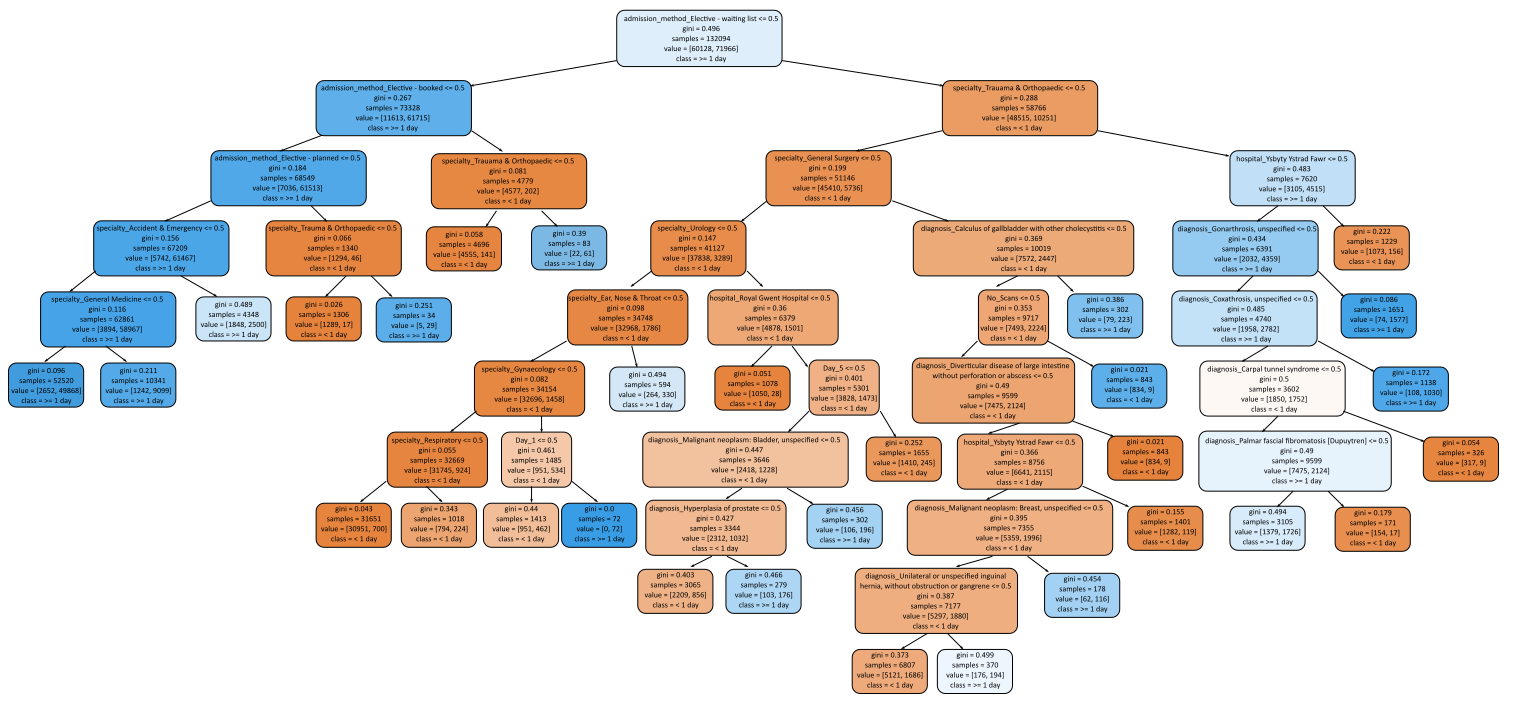
\includegraphics[scale=0.62]{Chapters/Chapter5/Figures/classificationtreevisual.png}
        \caption{Classification Tree Predicting Grouped LOS for Patients Within ABUHB}
        \label{fig:finalclasstree}
    \end{figure}
\end{landscape}


\subsubsection{Random Forests}

The CART model parameters that yielded the best results, were then implemented into a random forest model to determine if there was an improvement in these scores.

\begin{table}[h!]
    \centering
    \begin{tabular}{lcc}\toprule
     \textbf{Parameter}    &\textbf{RandomForestRegressor} & \textbf{RandomForestClassifier}  \\\midrule
       criterion  & ``squared\_error'' & ``gini'' \\
       max\_depth & None & None \\
       min\_samples\_split & 2 & 2 \\
       min\_samples\_leaf & 100 & 1\\
       min\_weight\_fraction\_leaf & 0 & 0 \\
       max\_features & None & None \\
       random\_state & None & None \\
       max\_leaf\_nodes & 30 & 30 \\
       min\_impurity\_decrease & 0 & 0 \\
       bootstrap & True & True\\
       oob\_score & False & False \\
       n\_jobs & None & None \\
       warm\_start & False & False \\
       ccp\_alpha & 0 & 0 \\
       max\_samples & None & None \\
       class\_weight & N/A & None \\\bottomrule
    \end{tabular}
    \caption{Selected Parameters for `RandomForestRegressor' and `RandomForestClassifier'}
    \label{tab:randomforest}
\end{table}

The variable `n\_estimators' underwent hyperparameter tuning to determine the value that produced the highest scores. This variable determines the number of trees to be used within the model. Typically in random forests, the larger the number of trees, the better the result produced, however, the higher the computational cost \cite{Pillai2020}.

\begin{table}[h!]
    \centering
    \begin{tabular}{ccccccccc}\toprule
       & \textbf{n\_estimators} &  10 & 20 & 30 & 40 & 50 \\\midrule
       \multirow{2}{*}{Regression} & R$^{2}$ Score &  0.342912 & 0.342917 & 0.343148 & 0.343291 &  0.343171\\
      &  Computational Time (s) &130.80 & 260.13 & 390.63 & 535.95 & 655.92\\ \midrule
        \multirow{2}{*}{Classification} & Accuracy & 0.883539 & 0.887809 & 0.8892296 & 0.890443 & 0.890928 \\
        & Computational Time (s) & 16.58 & 19.37 & 27.72& 36.87& 37.88\\\bottomrule
        
    \end{tabular}
    \caption{Random Forest Results}
    \label{tab:RandomForestResults}
\end{table}

Table \ref{tab:RandomForestResults} displays the random forest results for the regression and classification experiments. The regression random forest increased the regression tree R$^{2}$ by 0.0491\% from 34.28\%. This was achieved by setting `n\_estimators' to 40, in a computational time of 535.95 seconds. Since there is only an increase of 0.0491\% and a computational increase of 508.9714 seconds, the trade off is not worth the additional increase in accuracy.

Additionally, the classification random forest did not improve the accuracy of the the model compared to the classification tree. There is a difference of 0.8\% in accuracy levels. One reason for this could be the optimal parameters for the random forest are not the same as those for the classification tree. 



% 34.28 - 26.9786
% 89.89 - 16.7448
%\hl{check accuracy of 40 and 50}
% [0.6937385875183382, 0.6935564779512825, 0.6934586279595261, 0.6938434142627203, 0.6935341465216683]
% 100 takes too long


% [0.34291178317877047, 0.3429167220132139, 0.3431484589021293, 0.3432914970401735, 0.34317072100455626]
% [130.8033800000003, 260.12614380000014, 390.6309390999995, 535.9524377999996, 655.9202118000003]

\subsection{Predictive Analytics Summary}
This section has discussed the application of predictive analytics to data within ABUHB. Linear and logistic regressions were firstly performed, detailing a variables influence for the variability in the LOS. Admission method, diagnosis and speciality categories were the most influencing factors in the LOS.

Regression trees were developed to identify groupings of patients in order to predict continuous LOS. Figure \ref{fig:finalregtree} displays the different groupings and classifications of patients LOS, with the average LOS for each group. A total of 30 groups were identified due to the `max\_leaf\_nodes' being equal to 30. This resulted in an R$^{2}$ value of 34.23\%.

Classification trees were then built with the groupings of discharged on day of arrival or admitted overnight (Figure \ref{fig:finalclasstree}). The best trade off solution between accuracy, precision, recall and computational time, was 30 `max\_leaf\_nodes' and one `min\_samples\_leaf', yielding an accuracy score of 89.89\%. Comparing the classification to regression trees showed there to be a 55.66\% improvement by grouping LOS into two groups.

The random forests were both computationally heavier in performance time but did not cause a large enough increase in the overall accuracy and R$^{2}$ scores. 

The CART models showed improvement on the simple linear and logistic regressions and therefore highlighting the benefits of using these techniques to predict patient classifications. The CART models will be linked with the prescriptive models (Section \ref{sec:prescriptiveresults}), in Section \ref{sec:linking}. Here, evaluation will take place into the benefits of using CART models over traditional averages. 


\section{Prescriptive Analytics Results}\label{sec:prescriptiveresults}
This section will look at the deterministic and two stage stochastic models developed in Chapter \ref{chp:presciptive}. The demographics of ABUHB will be used in order to determine the most efficient way to organise specialties and nursing staff amongst a network of hospitals.


\subsection{Model Data}
The deterministic and two-stage stochastic models require user inputs to generate results. In total, the deterministic model requires eleven variables, whereas the two-stage stochastic model requires 17 variables.
Discussion around the selection of these variables will take place in Sections \ref{subsec:hospandregions} to \ref{sec:ABUHBstaffing}. A complete list of the variables used within the models can be found within Table \ref{tab:appdetermpa} for the deterministic model and Table \ref{tab:appstochpa} for the two-stage stochastic model in the Appendix.

\subsubsection{Hospitals and Regions}\label{subsec:hospandregions}
Within ABUHB, there are ten hospitals located within the five regions as discussed in Section \ref{sec:ABUHB}. In addition, the data contained an additional four medical sites where patients receive treatment. It is important to include patients attending these sites within the model to ensure the entire demand is included and sufficient beds and staff are planned. Table \ref{tab:ABUHBregionhospitals} displays the six regions included in the model and their associated hospitals.
\begin{table}[h!]
    \centering\scalebox{0.9}{
    \begin{tabular}{ll}\toprule
       \textbf{Region}  &  \textbf{Hospitals}\\\midrule
       \multirow{2}{*}{Region 1 (Newport) } & Royal Gwent Hospital, St Woolos Acute Hospital, \\ & St Woolos Community Hospital \\ 
       Region 2 (Caerphilly) & Ysbyty Ystrad Fawr, Rhymney Integrated Health and Social Care Centre\\
       Region 3 (Blaenau Gwent) & Ysbyty Aneurin Bevan\\
       Region 4 (Torfaen)& County Hospital\\
       \multirow{2}{*}{Region 5 (Monmouthshire)}& Nevill Hall Hospital, Chepstow Community Hospital, \\
       &Monnow Vale Integrated Health and Social Care Centre\\
       Other & University Hospital of Wales, Offsite, Outsource, Outsource - CareUK\\\bottomrule
    \end{tabular}}
    \caption{ABUHB Hospitals and Their Associated Regions}
    \label{tab:ABUHBregionhospitals}
\end{table}

The parameter UB$_{h}^{\textnormal{max, bed, 1st}}$ was determined from online publicly available data recorded by the Welsh Government \cite{StatsWales2021}. The Welsh Government record, over a year period, the average daily beds available for each specialty in each hospital. Within the 10 main hospitals, a total of 1,704 beds were available per day to the entire population. Therefore the maximum number of beds available will be scaled to represent the proportion of elderly admitted. For the four additional hospitals, which are either not at a hospital site or outside the trust, a fixed value of 20 was given. For the second stage maximum number of beds,  UB$_{h}^{\textnormal{max, bed, 2nd}}$, an additional 10\% of beds will be able to be made available, either by opening additional wards, transferring patients to other hospitals in the region, or to temporarily have patients waiting in corridors for permanent beds.

\subsubsection{Hospitals and Specialties}
ABUHB provides 29 different specialties among the fourteen hospital and care locations. This results in a combination of 406 unique hospital and specialty combinations. However, in practice, there are 90 combinations of hospital and specialty locations (Found in Figure \ref{fig:hospspec} and Appendix \ref{App:Hospitals}). These locations will determine the value of $K_{s,h}$. If a specialty is able to open in a hospital then the value will be equal to the UB$_{h}^{\textnormal{max,bed}}$, otherwise the value is zero. This therefore has the assumption that if a specialty can open, the hospital can choose to open all their beds to that specialty.

Online publicly available data was used for the costings per specialty from Public Health Scotland \cite{PHS2021}. The Scottish population follows a similar demographic to those in Wales and has similar operational running costs within hospitals. Additionally, the health boards in Scotland contain a variety of community and acute hospitals. Table \ref{tab:PHSCostsPerSpecialty} displays the minimum, maximum and weighted average cost for each specialty in the 2019 - 2020 financial year. In order to determine similar costings for hospitals within ABUHB, specialty cost values per hospital were randomly generated within the range of the Scottish data. Additionally, the values produced the same weighted average as the Scottish data. Some specialties in ABUHB did not overlap with the Scottish data, and therefore the category, `Medical Other', was selected for these specialties (anaesthetics, community medicine, diabetes and endocrinology and radiology). To determine the second stage hospital costs, c$_{s,h}^{\textnormal{bed, 2nd}}$, an additional 20\% was added each of the c$_{s,h}^{\textnormal{bed, 1st}}$ values.
\begin{table}[h!]
    \centering
    \begin{tabular}{lccc}\toprule
        \textbf{Specialty} & \textbf{Minimum Cost} & \textbf{Weighted Average} & \textbf{Maximum Cost} \\\midrule
        Accident \& Emergency & $\pounds$22 &$\pounds$247 &$\pounds$924 \\
        Anaesthetics & $\pounds$34 & $\pounds$1,021 & $\pounds$2,370\\
        Cardiology & $\pounds$4 & $\pounds$614 & $\pounds$1,513 \\
        Care of the Elderly & $\pounds$131 & $\pounds$577 & $\pounds$6,021 \\
        Community Medicine & $\pounds$34 & $\pounds$1021 & $\pounds$2,370\\
        Dermatology & $\pounds$203 & $\pounds$1,381 &$\pounds$2,446 \\
        Diabetes \& Endocrinology & $\pounds$34 & $\pounds$1,021 & $\pounds$2,370\\
        Ear, Nose \& Throat & $\pounds$77 & $\pounds$491 & $\pounds$1,436 \\
        Gastroenterology & $\pounds$112 & $\pounds$656 & $\pounds$1,472 \\
        General Medicine & $\pounds$2 & $\pounds$290 & $\pounds$1,418\\
        General Surgery & $\pounds$11 & $\pounds$541 & $\pounds$1,517\\
        GP Other & $\pounds$6& $\pounds$325 & $\pounds$1,117\\
        Gynaecology & $\pounds$180 & $\pounds$517 & $\pounds$2,526 \\
        Haematology & $\pounds$411 & $\pounds$1,208 & $\pounds$5,214 \\
        Infectious Diseases & $\pounds$438 &$\pounds$711 & $\pounds$1,188 \\
        Intermediate Care & $\pounds$0 & $\pounds$118 & $\pounds$361 \\
        Maxillo-Facial & $\pounds$96 & $\pounds$1,410 & $\pounds$8,637 \\
        Neurology & $\pounds$620 & $\pounds$1,273 & $\pounds$3,260 \\
        Ophthalmology & $\pounds$166 & $\pounds$729 & $\pounds$10,895 \\
        Pain &$\pounds$6 & $\pounds$128 & $\pounds$865 \\
        Plastic Surgery & $\pounds$179 & $\pounds$902 & $\pounds$1,399 \\
        Radiology & $\pounds$34 & $\pounds$1,021 & $\pounds$2,370\\
        Radiotherapy and Oncology & $\pounds$48 & $\pounds$1,089 & $\pounds$2,182 \\ 
        Rehabilitation & $\pounds$58 & $\pounds$1,455 & $\pounds$30,305 \\
        Respiratory & $\pounds$75 & $\pounds$448 & $\pounds$1,818 \\
        Restorative Dentistry & $\pounds$1 & $\pounds$140 & $\pounds$178 \\
        Rheumatology & $\pounds$155 & $\pounds$596 & $\pounds$1,256 \\
        Trauma and Orthopaedic & $\pounds$4 & $\pounds$703 & $\pounds$1,633 \\
        Urology & $\pounds$77 & $\pounds$379 & $\pounds$17,899 \\ \bottomrule
    \end{tabular}
    \caption{NHS Scotland Minimum, Weighted Average and Maximum Costs per Specialty \cite{PHS2021}}
    \label{tab:PHSCostsPerSpecialty}
\end{table}
%Anaesthetics, Community Medicine, Diabetes and Endocrinology, radiology,


\subsubsection{Staffing}\label{sec:ABUHBstaffing}
Within the NHS, there are different levels of experience within nursing \cite{NHS2022}. Typically on a ward there will be a mixture of different bands of nurses to make up the team of nurses. It is also important to ensure there is a mixture of different skill sets on a ward at a time \cite{Jones2015}. Typically, the registered nurse to patient ratio ranges from 1:1 to 1:10. The most critical patients require more direct care from nurses, i.e., intensive care units often have required ratios of one nurse to either one or two patients \cite{Kean2013}. Within general inpatient wards this ratio varies. The ratio of nurses to patients will vary between different specialities, with the more acute specialities requiring more nurses to patients. It will be assumed that an equal number of nurses across the bands will be required on the wards, with each band required to meet a given ratio.

This model will be developed with three levels of nursing bands (five, six and seven \cite{East2014}). The hourly pay for each band varies with experience, with Table \ref{tab:nhsbands} displaying the intermediate salary \cite{NHSEmployers2021}. When there is insufficient staffing levels, bank or agency staff are required. These nurses 
have a higher hourly wage, due to the unreliability of shifts \cite{OHNFT2023}. 

\begin{table}[h!]
    \centering
    \begin{tabular}{cccc}\toprule
         & \textbf{Band 5} & \textbf{Band 6} & \textbf{Band 7} \\\midrule
       c$^{\textnormal{staff,1st}}_{b}$  & $\pounds$14.21 & $\pounds$17.48 & $\pounds$21.54 \\
         c$^{\textnormal{staff,2nd}}_{b}$ & $\pounds$18.95 & $\pounds$23.36 &  $\pounds$27.42 \\ \bottomrule
    \end{tabular}
    \caption{NHS Hourly Staffing Costs per Band}
    \label{tab:nhsbands}
\end{table}

As of June 2022, ABUHB employed approximately 1,935 registered adult and general nurses \cite{StatsWales2022}. This value includes all bands of nurses across all specialties. For the purpose of the model, it will be assumed that 600 nurses are available, 200 for each band. Similarly, for the variable UB$^\textnormal{max, staff, 2nd}_b$, it will be assumed that up to 100 additional nurses for each can be requested from bank for each band.

%https://statswales.gov.wales/Catalogue/Health-and-Social-Care/NHS-Staff/Non-Medical-Staff/nursingmidwiferyandhealthvisitingstaff-by-grade-areaofwork-year


%file:///C:/Users/C1503449/Downloads/NursestaffinglevelsprojectreportPUBLversion.pdf Technical report jones2015

\subsection{Model Development}
These variables will be implemented into models developed in both Microsoft Excel using the OpenSolver add-in and Python using the PuLP packages as a solver. Microsoft Excel was selected as a primary tool, since it is familiar within the health board and open-source. The OpenSolver add-in was used over the built in Excel solver, due to the limitations  on the number of decision variables and constraints. OpenSolver has previously been used within healthcare planning for both bed planning \cite{Lal2015} and staff allocation \cite{Respicio2018}. A Python tool was additionally developed as it allows for flexibility within the number of hospitals, specialties and band levels of nurses. This adaptability ensures the model is dynamic to the changing needs and demographics of the health board. Python is also open-source, adaptable and easy to learn \cite{Ranum2006}, which will enable future development by senior staff at ABUHB. 

Both tools utilise the COIN-OR (Computational Infrastructure for Operations Research) 
optimisation engine. COIN-OR is a project managed by the COIN-OR Foundation with the aim to provide an ``open-source community for operations research software'' \cite{COF2016, LougeeHeimer2003}. The COIN-OR project consists of numerous smaller initiatives, including the development of various software for a variety of problems, methods, and coding languages. The COIN-OR community has developed two main linear programming solvers: CLP (COIN-OR Linear Programming), which primarily uses the simplex method as its core algorithm, and CBC (COIN-OR Branch and Cut), a mixed integer linear program-based (MILP) branch and cut library that also makes use of CLP. Although both of these solvers are designed in C++, they can be used with different languages through readily available packages such as PuLP. Since the deterministic and two-stage stochastic models developed require the decision variables to be integer, the CBC solver is the most suitable choice.

COIN-OR solvers are free and open source which is vital for ABUHB as the minimisation of cost is a necessity for the organisation. There exists more advanced commercial software including CPLEX \cite{IBM} and Gurobi \cite{GurobiOptimization}, these were not considered due to the significant associated license cost. 

\subsection{Microsoft Excel OpenSolver Results}\label{sec:opensolverresult}
Microsoft Excel OpenSolver provides the option to change certain parameters in order to increase accuracy and to limit runtime. There are four parameters available for the user to change:
\begin{itemize}
    \item Maximum Solution Time (seconds)
    \item Branch and Bound Tolerance (\%)
    \item Maximum Number of Iterations
    \item Precision
\end{itemize}

The maximum solution time option determines how the long the programme is allowed to run before the model is stopped. Within this analysis, a maximum solution time was set to 100 seconds, however the optimum was reached prior to this. The branch and bound tolerance determines the stopping percentage that enables the solver to stop if it has found a feasible integer solution whose objective function is within the given percentage of the true integer optimal solution. All models were run on a branch and bound tolerance of 0.01\%. The maximum number of iterations determines the how many iterations the solver will use, which was left unbounded. Finally, precision was set to a value of 0.000001. The precision determines the accuracy of the optimal solution. The larger the number indicates a lower degree of precision, however a larger degree of precision the more time Solver will take to reach solutions.


\subsubsection{Experiment 1 - Three Years Worth of Data}
The first experiment examines the entire three years worth of data from April 2017 to March 2020, to determine the daily average number of beds and staff required.

Recall the following equations discussed in Chapter \ref{chp:presciptive}, which were used to calculate the daily demand for each region. 

\begin{align}
     \text{Average beds}_{s,h} &= \text{Average LOS}_{s,h} * \text{Average demand}_{s,h}\tag{\ref{eq:averagebeds1} revisited}\\
      \text{Average beds}_{s,r} &= \sum_{h \in \mathcal{R}} \text{Average beds}_{s,h} \tag{\ref{eq:averagebeds2} revisited}
\end{align}

Using these equations against the whole data set, resulted in Table \ref{tab:regionaldemands1} which displays the average daily demand for each specialty in each of the six regions. The demands are rounded to four decimal places, however, since beds have to be integer, the model will round these to the nearest integer.

\begin{table}[h!]
    \centering\scalebox{0.75}{
    \begin{tabular}{lcccccc}\toprule
     \textbf{Specialty}    & \textbf{Region 1} & \textbf{Region 2} & \textbf{Region 3} & \textbf{Region 4} & \textbf{Region 5} & \textbf{Region 6}  \\ \midrule
Accident \& Emergency	& 2.1081& 	0& 	0& 	0& 	9.1846	& 0 \\
Anaesthetics & 	4.6079	& 0& 	0& 	0& 	0& 	0 \\
Cardiology & 	16.0947	& 0& 	0& 	0& 	9.8809& 	0.0002 \\
Care of the Elderly	& 94.5387	& 57.7380	& 0.7489& 	8.7416	& 46.4786	& 0\\
Community Medicine& 	0& 	6.9952&	0& 	0.3121& 	12.9756	& 0\\
Dermatology& 	2.4192	& 0& 	0& 	0& 	0& 	0\\
Diabetes \& Endocrinology& 14.5635	& 21.2838	& 0& 	0& 	17.2387& 0\\
Ear Nose \& Throat	& 3.2480	& 0.0041	& 0	& 0	& 0	& 0\\
Gastroenterology& 	13.0208	& 0.6065	& 0	& 0& 	20.1331& 	0.0725\\
General Medicine& 	84.9712& 	0.9846	& 0.0115	& 0& 	14.1695& 	0\\
General Surgery& 	46.5808& 	0.5390	& 0& 	0& 	21.8943& 	0.0006 \\
GP Other& 	0& 	9.8734&0& 	0& 	15.2880& 	0\\
Gynaecology& 	2.1194	& 0.1222	& 0& 	0& 	1.1716& 	0.0002\\
Haematology& 	3.0718	& 0.0320	& 0& 	0& 	1.8339& 	0.0002\\
Infectious Diseases	& 7.1817& 	0& 	0& 	0& 	0& 	0\\
Intermediate Care& 	0& 	0& 	0.3426	& 0.3248	& 0 & 	0 \\
Maxillo-Facial	& 1.1831	& 0& 	0& 	0& 	0.0243& 	0\\
Neurology	& 1.5828	& 0	& 0	& 0& 	0	&0\\
Ophthalmology& 	2.5538& 	0.0028& 	0& 	0& 	0.1968	& 0.5232\\
Pain& 	0.0586& 	0.0055& 	0& 	0.0037& 	0.0131& 	0 \\
Plastic Surgery	& 0& 	0& 	0& 	0	& 0.0336	& 0.0002\\
Radiology& 	0.0146	& 0& 	0& 	0 & 	0.0026	& 0\\
Radiotherapy \& Oncology& 	0.2265& 	0& 	0& 	0& 	0& 0\\
Rehabilitation	& 62.8610	& 32.9653	& 68.9710& 	31.9917	& 24.4659	& 0 \\
Respiratory& 	29.8010& 	0& 	0& 	0& 	27.8372	& 0 \\
Restorative Dentistry& 	0.0001	& 0& 	0& 	0& 	0& 	0\\
Rheumatology& 	0.0004& 	0.001& 5	0& 	0& 	0.0128& 	0\\
Trauma \& Orthopaedic	& 60.3126& 	0.6665	& 0& 	0& 	41.5186& 	0\\
Urology& 	12.3397& 	0.0521	& 0& 	0& 	0.2034& 	0.0702\\
\bottomrule
   
    \end{tabular}}
    \caption{Regional Daily Demands for Three Years of ABUHB Patient Admissions to Four Decimal Places}
    \label{tab:regionaldemands1}
\end{table}





\subsubsubsection{Deterministic Model}
In order to meet the demand and satisfy the constraints, the deterministic model utilised the first stage variables only (Table \ref{tab:appdetermpa}). The results yielded a daily cost of $\pounds$1,011,291.52
 in 1.47 seconds. In total, 1026 beds across the health board were deployed with Figure \ref{fig:detHeatmap1} displaying the precise locations of these beds. In order to satisfy demand a total of 621 NHS nurses across a 24 hour period were required.


\begin{figure}[h!]
    \centering
    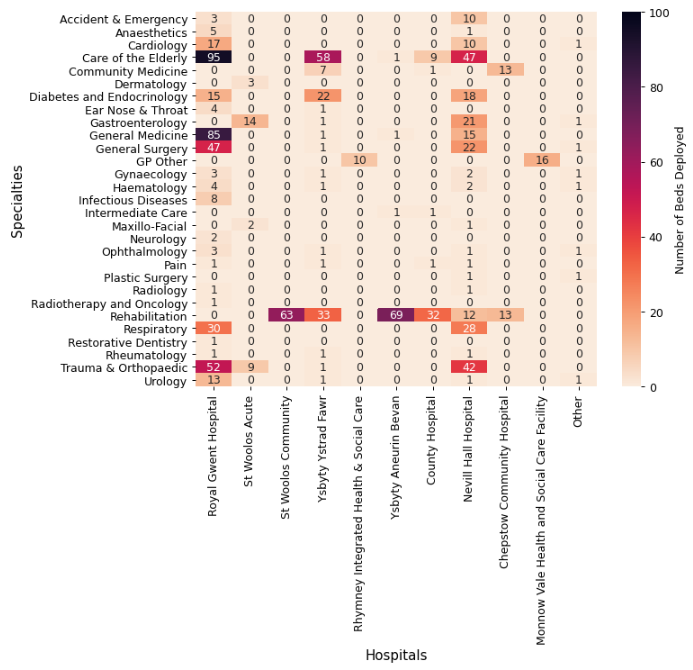
\includegraphics{Chapters/Chapter5/Figures/exdet.png}
    \caption{Heatmap of bed locations for each specialty within each hospital - Deterministic Results - Experiment 1 - Excel OpenSolver}
    \label{fig:detHeatmap1}
\end{figure}


\subsubsubsection{Two-Stage Stochastic Model}
The two-stage stochastic model was considered with four different scenarios. Table \ref{tab:scenarios1} displays each of the four scenarios and their associated probabilities. The average of all scenarios are equal to the deterministic daily demands (Table \ref{tab:regionaldemands1}). The variable values can be seen within Table \ref{tab:appstochpa}. 

\begin{table}[h!]
    \centering
    \begin{tabular}{@{}cc@{}}\toprule
       \textbf{Scenario}  &\textbf{Probability}  \\\midrule
       Demand Increases by 5\% & 25\% \\ 
       Demand Increases by 10\% & 25\% \\
       Demand Decreases by 5\% & 25\% \\ 
       Demand Decreases by 10\% & 25\% \\\bottomrule
    \end{tabular}
    \caption{Four Scenarios for the Two-Stage Stochastic Model}
    \label{tab:scenarios1}
\end{table}

Figure \ref{fig:graphstoch1} displays the objective function compared to computational run time. If the model did not have the time restriction, the objective value function was $\pounds$1,049,699.1 after 106.38 seconds. The model reaches the optimal objective function within 90.93 seconds. For analysis and comparisons with the python models the maximum computational runtime was set to 100 seconds.

\begin{figure}[h!]
    \centering
    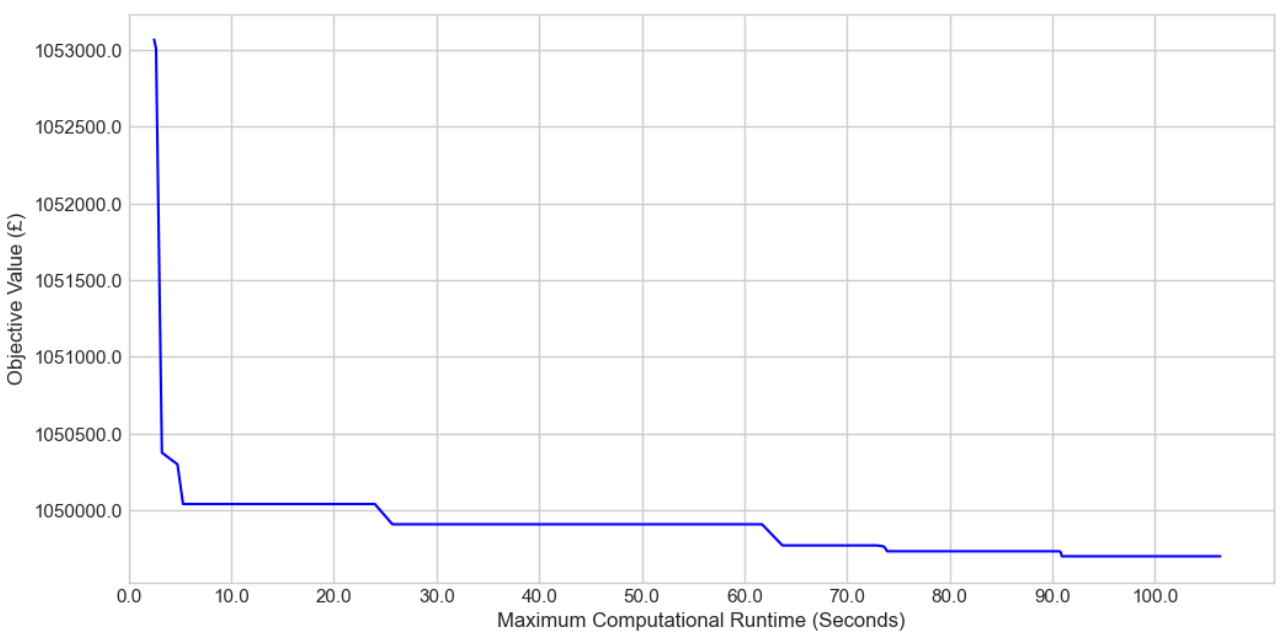
\includegraphics[width=12cm]{Chapters/Chapter5/Figures/StochasticRunTime.png}
    \caption{Objective Function Value against Maximum Computational Runtime For Two-Stochastic Model - Experiment 1}
    \label{fig:graphstoch1}
\end{figure}


Table \ref{tab:dettwostageresults1} compares the results for the deterministic and two-stage stochastic models. 

The two-stage stochastic model deployed an additional 105 beds compared to the deterministic model, deploying 1003 in the first stage and a maximum of 128 in the second stage. Similarly, 75 additional nurses were deployed. The objective value increased by 3.8\%, to a daily cost of $\pounds$1,049,699.10.



\begin{table}[h!]
    \centering
    \begin{tabular}{cccccl}\toprule
 & \multicolumn{2}{l}{\textbf{Total Beds}} & \multicolumn{2}{c}{\textbf{Total Staff}} & \multirow{2}{*}{\textbf{Objective Value ($\pounds$)}}\\ \cmidrule(lr){2-3} \cmidrule(lr){4-5}
 & xbed           & ubed          & xstaff         & ustaff         \\ \midrule
      Deterministic & 1026 & - &  621 & - & 1,011,291.52 =  EV \\ \midrule
      Stochastic & 1003 & 128  & 603 & 93 & 1,049,699.10 = RP\\ \bottomrule
    \end{tabular}
    \caption{Deterministic and Two-Stage Stochastic Results - Experiment 1 - Excel OpenSolver}
    \label{tab:dettwostageresults1}
\end{table}

The location of each the 1131 beds can be seen within Figure \ref{fig:stocHeatmap1}.

\begin{figure}[h!]
    \centering
    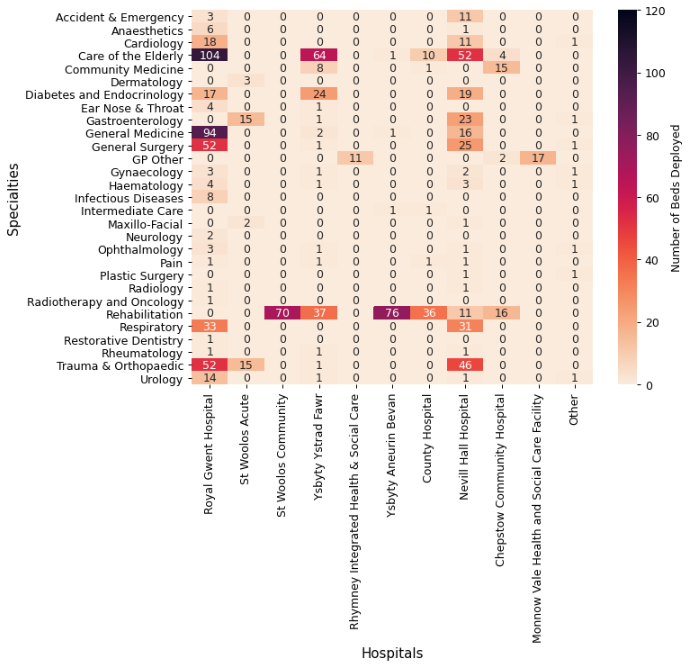
\includegraphics{Chapters/Chapter5/Figures/exsto.png}
    \caption{Heatmap of bed locations for each specialty within each hospital - Two-Stage Stochastic Results - Experiment 1 - Excel OpenSolver}
    \label{fig:stocHeatmap1}
\end{figure}





\subsubsubsection{Test A}
The first test as discussed in Section \ref{sec:TestA} involves using the results from the deterministic model and fixing these as the first stage variables in the two-stage stochastic model. Table \ref{tab:eevdettwostageresults1} displays the results for the VSS. 

\begin{table}[h!]
    \centering
    \begin{tabular}{cccccl}\toprule
 & \multicolumn{2}{l}{\textbf{Total Beds}} & \multicolumn{2}{c}{\textbf{Total Staff}} & \multirow{2}{*}{\textbf{Objective Value ($\pounds$)}}\\ \cmidrule(lr){2-3} \cmidrule(lr){4-5}
 & xbed           & ubed          & xstaff         & ustaff         \\ \midrule
      Deterministic & 1026 & - &  621 & - & 1,011,291.52 =  EV \\ \midrule
      Stochastic & 1003 & 128  & 603 & 93 & 1,049,699.10 = RP\\ \midrule
      Test A & 1026 & 101 & 547&  99 &  1,070,745.34 = EEV \\\bottomrule
    \end{tabular}
    \caption{EEV, Deterministic and Two-Stage Stochastic Results - Experiment 1 - Excel OpenSolver}
    \label{tab:eevdettwostageresults1}
\end{table}

The VSS can be calculated to be 2\%, equating to $\pounds$21,046.24 per day. Whilst a value of $\approx$ 2\% is low, the saving over a year period equates to $\pounds$7,681,877.60. This shows that there is a benefit in using the stochastic solution over the deterministic solution.

To understand why the deterministic solution is performing poorly, we can calculate the LUSS and LUDS values. This will determine whether the model is too optimistic or the locations of beds and staff are incorrect.



\subsubsubsection{Test B}
The second test discussed in Section \ref{sec:TestB}, involves fixing the first stage variables which are at zero or the lower bound in the deterministic problem, and then to solve in the stochastic programme. In this case, there are hospitals, which even though beds can be deployed, the value is zero. This will determine if the deterministic model produced the correct, non-zero variables.

Recalling Equation \eqref{eq:LUSS}, the RP result can then be compared to the EESV.

\begin{equation}
    LUSS = ESSV - RP\tag{\ref{eq:LUSS} revisited}
\end{equation}

\begin{table}[h!]
    \centering
    \begin{tabular}{cccccl}\toprule
 & \multicolumn{2}{l}{\textbf{Total Beds}} & \multicolumn{2}{c}{\textbf{Total Staff}} & \multirow{2}{*}{\textbf{Objective Value ($\pounds$)}}\\ \cmidrule(lr){2-3} \cmidrule(lr){4-5}
 & xbed           & ubed          & xstaff         & ustaff         \\ \midrule
      Deterministic & 1026 & - &  621 & - & 1,011,291.52 =  EV \\ \midrule
      Stochastic & 1003 & 128  & 603 & 93 & 1,049,699.10 = RP\\ \midrule
      Test A & 1026 & 101 & 621&  111 &  1,070,745.34 = EEV\\\midrule
      Test B & 1026 & 101 & 621&  111 &  1,070,745.34 = EESV\\ \bottomrule
    \end{tabular}
    \caption{ESSV, EEV, Deterministic and Two-Stage Stochastic Results - Experiment 1 - Excel OpenSolver}
    \label{tab:eesveevdettwostageresults1}
\end{table}

The results in Table \ref{tab:eesveevdettwostageresults1} show that LUSS value is calculated to be $\pounds$21,046.24. This means that the LUSS and VSS values are equal, and the stochastic programme chooses not to change the value of any of the variables. Therefore, it can be concluded that the deterministic solution is poor since it deploys the incorrect number of beds and staff to the hospital locations.

\subsubsubsection{Test C}
The final test determines the upgradeability of the model by adding the number of beds and staff deployed in the deterministic model as a constraint, for the stochastic model (Section \ref{sec:TestC}). 

\begin{table}[h!]
    \centering
    \begin{tabular}{cccccl}\toprule
 & \multicolumn{2}{l}{\textbf{Total Beds}} & \multicolumn{2}{c}{\textbf{Total Staff}} & \multirow{2}{*}{\textbf{Objective Value ($\pounds$)}}\\ \cmidrule(lr){2-3} \cmidrule(lr){4-5}
 & xbed           & ubed          & xstaff         & ustaff         \\ \midrule
      Deterministic & 1026 & - &  621 & - & 1,011,291.52 =  EV \\ \midrule
      Stochastic & 1003 & 128  & 603 & 93 & 1,049,699.10 = RP\\ \midrule
      Test A & 1026 & 101 & 621&  111 &  1,070,745.34 = EEV\\\midrule
      Test B & 1026 & 101 & 621&  111 &  1,070,745.34 = EESV\\\midrule
      Test C & 1042 & 86 &  207  & 78 &  1,065,666.86 = EIV \\\bottomrule
    \end{tabular}
    \caption{EIV, ESSV, EEV, Deterministic and Two-Stage Stochastic Results - Experiment 1 - Excel OpenSolver}
    \label{tab:eiveesveevdettwostageresults1}
\end{table}

The LUDS value is calculated by the difference between EIV and RP, which using Table \ref{tab:eiveesveevdettwostageresults1}, determines this value to be $\pounds$15,967.76. Since LUDS $<$ VSS, this demonstrates partial upgradeability and additional beds and staff are deployed in the first stage compared to the deterministic solution.

\subsubsubsection{Summary}
This section has analysed bed and staffing requirements based on three years worth of data, using the daily demand average. The VSS has shown that there is a 2\% saving per day using costings from NHS Scotland \cite{PHS2021}, equalling $\pounds$7,681,877.60 per year. Any additional potential savings that can saved by the NHS are critically important. 

In conclusion, the deterministic solution does not perform well in a stochastic environment because too few beds and staff are deployed (1,026 beds and 621 staff compared to 1,131 beds and 696 staff). As $EESV = EEV$ and $LUSS=VSS$, the deterministic solution has a bad structure with required units for the stochastic environment are closed. Therefore, this shows there is evidence for the NHS to move away from simply planning on averages and use more sophisticated techniques with the potential for large cost savings.


\subsubsection{Experiment 2}
The second experiment will analyse the beds on a year to year basis, to determine if there are yearly differences on the number and beds that should be deployed. Since the yearly demand of patients contained little variation (Section \ref{sec:datatrends}), from a high level, it could be assumed that the beds and staff required would contain little variation. This experiment will therefore determine if there is the need to plan on a smaller scale horizon.  %It will also be investigated that if beds are planned in year one, how this will effect the beds in year two and year three. \hl{Check this is what I do?}
Tables \ref{tab:regionaldemandsexp2a} and \ref{tab:regionaldemandsexp2b} display the regional demands for each speciality for each year. The same first stage (Table \ref{tab:appdetermpa}) and second stage (Table \ref{tab:appstochpa}) variables will be used as those in Experiment one to allow direct comparisons in Section \ref{sec:ExcelComparisons}.

\begin{landscape}

\begin{table}[h!]
    \centering\scalebox{0.8}{
    \begin{tabular}{lcccccccccccccccccc}\toprule
\multirow{2}{*}{\textbf{Specialty}}& \multicolumn{3}{c}{\textbf{Region 1}} & \multicolumn{3}{c}{\textbf{Region 2}}& \multicolumn{3}{c}{\textbf{Region 3}}\\\cmidrule(lr){2-4} \cmidrule(lr){5-7}\cmidrule(lr){8-10}
& \textbf{2017-2018} & \textbf{2018-2019} & \textbf{2019-2020} & \textbf{2017-2018} & \textbf{2018-2019} & \textbf{2019-2020} & \textbf{2017-2018} & \textbf{2018-2019} & \textbf{2019-2020} \\\midrule
%2017R1	2018R1	2019R1	2017R2	2018R2	2019R2	2017R3	2018R3	2019R3	2017R4	2018R4	2019R4	2017R5	2018R5	2019R5	2017R6	2018R6	2019R6
Accident \& Emergency &2.2703&	2.2025&	1.8524&	0&	0&	0&	0&	0&	0\\
Anaesthetics&4.5049&	4.4998&	4.8186	&0	&0&	0&	0&	0&	0	\\
Cardiology&17.2662&	14.6579&	16.3594&	0&0	&0&	0	&0&	0	\\
Care of the Elderly&76.9707	&88.5761&	118.0052&	55.7326&	58.4843	&58.9937&	0	&0.3977&	1.8461\\
Community Medicine&0	&0&	0&	7.1593&	6.0895&	7.7349&	0&	0	&0\\
Dermatology&2.8287	&2.1355&	2.2939&	0&	0	&0&	0&	0	\\
Diabetes \& Endocrinology&16.7264&	11.5043	&15.4574	&24.7432	&19.8417&19.2722	&0	&0	&0	\\
Ear, Nose \& Throat&3.0791	&3.7301&	2.9358	&0.0084	&0.0027&	0.0013	&0	&0&	0		\\
Gastroenterology&12.1823	&10.4803	&16.3906	&0.6416&	0.5303&	0.6478	&0	&0&	0	\\
General Medicine&106.1909	&96.5455&	52.2668&	0.2873	&1.1528&	1.5126&	0	&0	&0.0344	0\\
General Surgery&48.8745&46.5117&	44.3624	&0.4163&	0.521	&0.6794	&0	&0	&0\\
GP Other&0	&0	&0	&9.6797	&10.1153	&9.8254	&0&	0&	0\\
Gynaecology&2.5425&	1.8482&	1.968&	0.1391&	0.1231&	0.1046&	0	&0	&0\\
Haematology&3.4524&	2.6894&	3.0736&	0	&0	&0.0959&	0	&0	&0\\
Infectious Diseases&8.1529&	6.4296&	6.9635&	0&	0	&0	&0	&0	&0	\\
Intermediate Care&0	&0&	0&	0&	0	&0&	0	&0.0078&	1.0184\\
Maxillo-Facial&1.2256	&1.0697	&1.2539&	0	&0	&0	&0&	0	&0\\
Neurology&1.4497	&1.565	&1.7336&	0&	0	&0&	0	&0	&0	\\
Ophthalmology  &2.5831	&2.4957	&2.5828&	0&	0	&0.0086	&0	&0&	0\\
Pain &0.0555	&0.066	&0.0545&	0&	0.0118	&0.0047	&0&	0	&0\\
Plastic Surgery&0	&0	&0	&0	&0&	0&	0	&0	&0\\
Radiology&0.0102	&0.0196	&0.0142	&0&	0&	0	&0	&0&	0\\
 Radiotherapy \& Oncology&0.0031	&0.0023	&0.673	&0	0	&0	&0	&0	&0\\
Rehabilitation&64.5703&	62.9902	&61.0276	&34.7587&	34.72&	29.427	&69.5287&	64.8741&	72.5009	\\
Respiratory&30.1523	&30.7641&	28.4902&	0	&0	&0	&0	&0	&0\\
Restorative Dentistry&0.0002	&0	&0.0002&	0	&0	&0	&0	&0	&0\\
Rheumatology&0	&0&	0.0011&	0	&0.0044&0	&0	&0	&0\\
Trauma \& Orthopaedic&57.1547	&61.7714&	62.0072&	0.7173	&0.6536&	0.6288&	0&	0	&0\\
Urology&11.4221	&13.5649&	12.033&	0.057	&0.0541&	0.0455&	0&	0	&0\\ \bottomrule

    \end{tabular}}
    \caption{Regions One, Two and Three Daily Demands for Three Individual Years of ABUHB Patient Admissions to Four Decimal Places}
    \label{tab:regionaldemandsexp2a}
\end{table}

\begin{table}[h! ]
    \centering\scalebox{0.8}{
    \begin{tabular}{lcccccccccccccccccc}\toprule
\multirow{2}{*}{\textbf{Specialty}}& \multicolumn{3}{c}{\textbf{Region 4}}& \multicolumn{3}{c}{\textbf{Region 5}}& \multicolumn{3}{c}{\textbf{Region 6}}\\\cmidrule(lr){2-4} \cmidrule(lr){5-7}\cmidrule(lr){8-10}\cmidrule(lr){11-13}\cmidrule(lr){14-16}\cmidrule(lr){17-19}
& \textbf{2017-2018} & \textbf{2018-2019} & \textbf{2019-2020} & \textbf{2017-2018} & \textbf{2018-2019} & \textbf{2019-2020} & \textbf{2017-2018} & \textbf{2018-2019} & \textbf{2019-2020}  \\\midrule

Accident \& Emergency&0	&0&	0	&8.5642	&10.0826	&8.9078&	0	&0	&0\\
Anaesthetics&0	&0&	0&	0.423&	0.7812	&1.1152&	0&	0&0\\
Cardiology&0	&0&	0&	10.7899	&10.2858&	8.5707	&0&	0&	0.0008\\
Care of the Elderly&12.3557	&6.4882&	7.3849	&53.7813&44.1656	&41.5028&	0&	0	&0\\
Community Medicine	&0.3653	&0.1386&	0.4321	&16.6726	&13.9982&	8.2691	&0&	0&	0\\
Dermatology	&0&	0	&0&	0&	0&	0	&0&0	&0\\
Diabetes \& Endocrinology	&0&	0	&0	&17.8653	&18.4154&	15.4405&	0&	0	&0\\
Ear, Nose \& Throat&0	&0&	0	&0	&0	&0	&0	&0	&0\\
Gastroenterology&0	&0	&0	&18.3652&	21.7402	&20.2937&	0.0006	&0	&0.0008\\
General Medicine&0	&0	&0	&12.0771	&11.8051	&18.6143&	0&	0&	0\\
General Surgery	&0&	0	&0	&21.656	&23.1851	&20.8447&	0.0003	&0.0003&	0.0008\\
GP Other	0	&0	&0&	14.7579&	13.86&	17.2409&	0	&0	&0\\
Gynaecology	&0	&0	&0	&1.2598&	1.5459&	0.7105	&0&	0&	0.0008\\
Haematology	&0	&0	&0	&1.8601	&1.7505&	1.8911	&0.0003&	0	&0\\
Infectious Diseases	&0	&0	&0	&0	&0	&0&	0&	0	&0\\
Intermediate Care&	0	&0.6014&	0.3729&	0&	0&	0&	0	&0&	0\\
Maxillo-Facial	&0	&0	&0&	0.0271&	0.0141	&0.0319	&0	&0	&0\\
Neurology	&0	&0	&0	&0&	0	&0	&0	&0	&0\\
Ophthalmology &0	&0	&0	&0.1748&	0.2065	&0.2093	&0	&0.0003	&0.0012\\
Pain &0.0086	&0.0008&	0.0016	&0.0145	&0.0156	&0.0094	&0&	0	&0\\
Plastic Surgery&	0	&0&	0	&0.0212&	0.0199	&0.06&	0	&0&	0.0008\\
Radiology&0	&0	&0	&0.006	&0.0003	&0.0017&	0&	0&	0\\
 Radiotherapy \& Oncology&	0&	0	&0&	0&	0&	0&	0&	0	&0\\
Rehabilitation&29.5590	&32.9368&	33.4754	&18.3286	&25.2346	&29.8199&	0&	0&	0\\
Respiratory&	0	&0	&0&	30.7903&29.5149	&23.2192	&0&	0	&0\\
Restorative Dentistry	&0&	0	&0	&0&	0&	0&	0&	0&	0\\
Rheumatology&0&	0&	0	&0	&0.0386&	0	&0	&0	&0\\
Trauma \& Orthopaedic&0	&0&	0	&42.5161	&41.2805&	40.7614&	0&	0&	0\\
Urology&0	&0&	0&	0.1685&	0.1933&	0.2485	&0.0028	&0.0027&	0.0035\\ \bottomrule

    \end{tabular}}
    \caption{Regions Four, Five and Six Daily Demands for Three Individual Years of ABUHB Patient Admissions to Four Decimal Places }
    \label{tab:regionaldemandsexp2b}
\end{table}
\end{landscape}

\subsubsubsection{Deterministic Model}
Using the average daily demands as the minimum number of beds that are required to be met, the deterministic model can run on each of the three years investigated. Table \ref{tab:detresults2} displays the number of beds and staff required each year with the expected daily cost per year. The year 2017 - 2018, has the largest expected cost, planning the largest number of beds and staff. By planning year by year, this has the potential for up to $\pounds$18,176.60 to be saved per day. 


\begin{table}[h!]
    \centering
    \begin{tabular}{ccccccl}\toprule
 & \multirow{2}{*}{\textbf{Year}}& \multicolumn{2}{l}{\textbf{Total Beds}} & \multicolumn{2}{c}{\textbf{Total Staff}} & \multirow{2}{*}{\textbf{Objective Value ($\pounds$)}}\\ \cmidrule(lr){3-4} \cmidrule(lr){5-6}
&& xbed           & ubed          & xstaff         & ustaff         \\ \midrule
     \multirow{3}{*}{Deterministic} & 2017 - 2018 & 1031 & - &  594 & - & 1,000,612.28 =  EV$_{17-18}$ \\ 
      & 2018 - 2019 & 1015 & - & 591 & - & 993,114.92 =  EV$_{18-19}$ \\
      & 2019 - 2020 & 1010 & - & 594 & - & 996,035.28 =  EV$_{19-20}$\\ \bottomrule
    \end{tabular}
    \caption{Deterministic Results - Experiment 2 - Excel OpenSolver}
    \label{tab:detresults2}
\end{table}

In order to visualise how these beds should be planned, Figure \ref{fig:detexp2} displays each of the three heatmaps for hospital and speciality locations. For the majority of locations, if hospital beds are opened then in the following years the beds remain open. The results also display, the number of patients which are required to be transferred to other non NHS site locations or hospitals in other healthboards through the ``Other'' category. Therefore if hospital managers want to limit the number of patients falling into the ``Other' category, they can determine how much additional demand they need to make available. In all three cases, a maximum of one additional bed is required per day for three to six specialities.
%\begin{landscape}

\begin{figure}
     \centering
     \begin{subfigure}[h!]{0.8\textwidth}
         \centering
         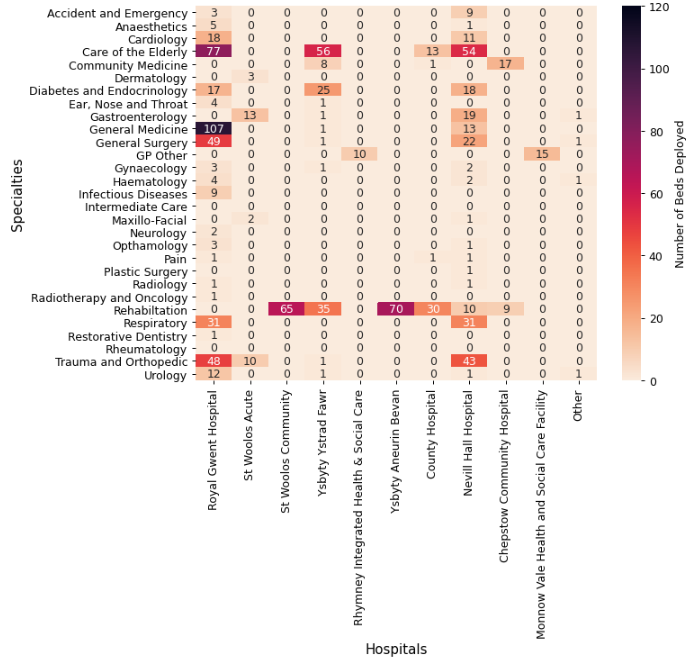
\includegraphics[width=\textwidth]{Chapters/Chapter5/Figures/2017DET.png}
         \caption{2017 - 2018}
         \label{fig:detexp2a}
     \end{subfigure}
\hfill
     \begin{subfigure}{0.8\textwidth}
         \centering
         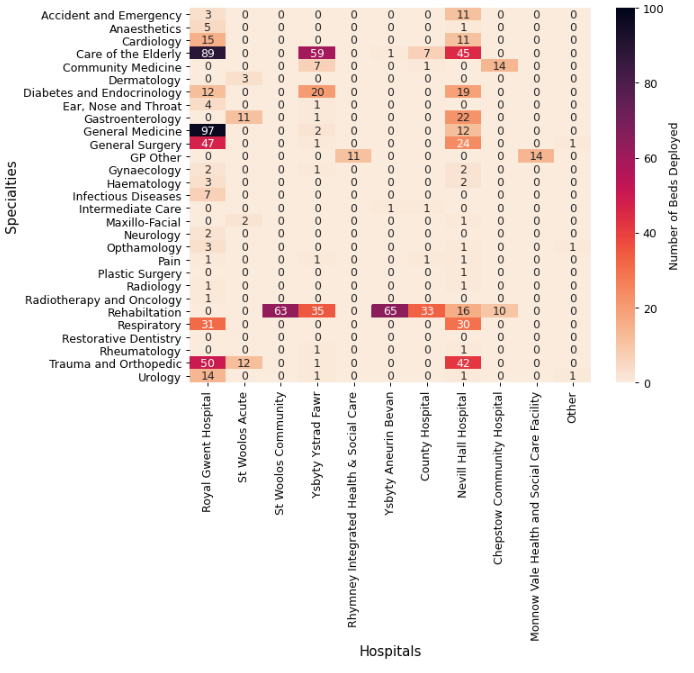
\includegraphics[width=\textwidth]{Chapters/Chapter5/Figures/2018DET.png}
         \caption{2018 - 2019}
         \label{fig:detexp2b}
     \end{subfigure}
     \end{figure}
\hfill
\begin{figure}\ContinuedFloat
     \begin{subfigure}{0.8\textwidth}
         \centering
         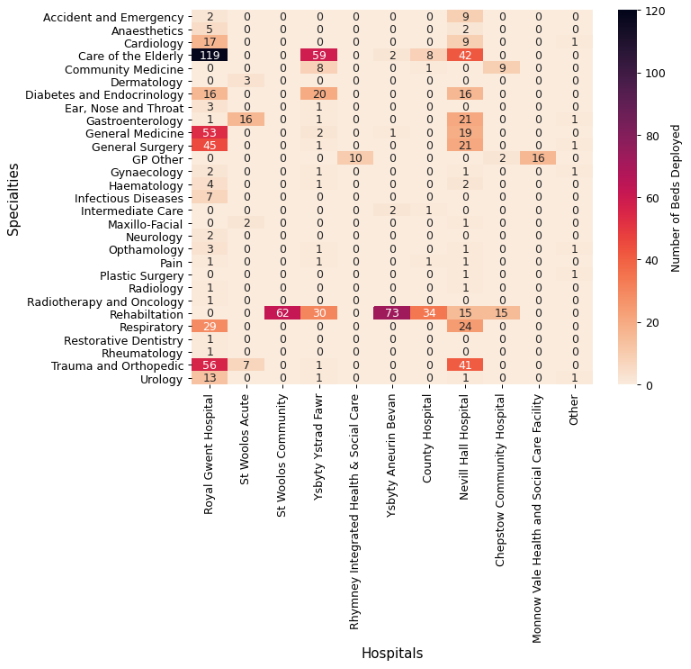
\includegraphics[width=\textwidth]{Chapters/Chapter5/Figures/2019DET.png}
         \caption{2019 - 2020}
         \label{fig:detexp2c}
     \end{subfigure}
        \caption{Heatmap of Bed Locations for Each Specialty Within Each Hospital by Year - Deterministic Results - Experiment 2 - Excel OpenSolver}
        \label{fig:detexp2}
\end{figure}

    
%\end{landscape}





\subsubsubsection{Two-Stage Stochastic Model}
The two-stage stochastic model was considered with the same four scenarios as in Table \ref{tab:scenarios1}. A maximum runtime was set for 100 seconds, although all computations were completed within 36 seconds. Table \ref{tab:detstocresults2} shows that in the first stage, fewer beds and staff are deployed compared to the deterministic result for all three years. This in turn, increases the objective value ranging from 3.31\% to 3.77\% , with a maximum of 124 and 96 additional beds and staff deployed respectively. 

\begin{table}[h!]
    \centering
    \begin{tabular}{ccccccl}\toprule
 & \multirow{2}{*}{\textbf{Year}}& \multicolumn{2}{l}{\textbf{Total Beds}} & \multicolumn{2}{c}{\textbf{Total Staff}} & \multirow{2}{*}{\textbf{Objective Value ($\pounds$)}}\\ \cmidrule(lr){3-4} \cmidrule(lr){5-6}
&& xbed           & ubed          & xstaff         & ustaff         \\ \midrule
     \multirow{3}{*}{Deterministic} & 2017 - 2018 & 1031 & - &  594 & - & 1,000,612.28 =  EV$_{17-18}$ \\ 
      & 2018 - 2019 & 1015 & - & 591 & - & 993,114.92 =  EV$_{18-19}$ \\
      & 2019 - 2020 & 1010 & - & 594 & - & 996,035.28 =  EV$_{19-20}$\\ \midrule
     \multirow{3}{*}{Stochastic} & 2017 - 2018 & 1006 & 123 & 573 & 90 & 1,036,584.08 =  RP$_{17-18}$ \\ 
      & 2018 - 2019 & 986 & 133 & 573 & 96 & 1,030,014.36 =  RP$_{18-19}$ \\
      & 2019 - 2020 & 979 & 134 & 564 & 99 & 1,026,981.72 =  RP$_{19-20}$\\ \bottomrule      
    \end{tabular}
    \caption{Deterministic and Two-Stage Stochastic Results - Experiment 2 - Excel OpenSolver}
    \label{tab:detstocresults2}
\end{table}

Figure \ref{fig:stocexp2} presents the locations of bed deployment for each specialty in each year. The largest differences can be seen when planning beds for RGH in the COTE and general medicine wards. A total of of 85 and 98 beds are each planned for COTE wards in 2017-2018 and 2018-2019 respectively, however the daily demand increases to 130 beds in the 2019-2020 period. Conversely, the general medicine daily bed requirement decreases from 117 and 107 in 2017-2018 and 2018-2019 respectively, to 58 in 2019-2020.

\begin{figure}
     \centering
     \begin{subfigure}[h!]{0.8\textwidth}
         \centering
         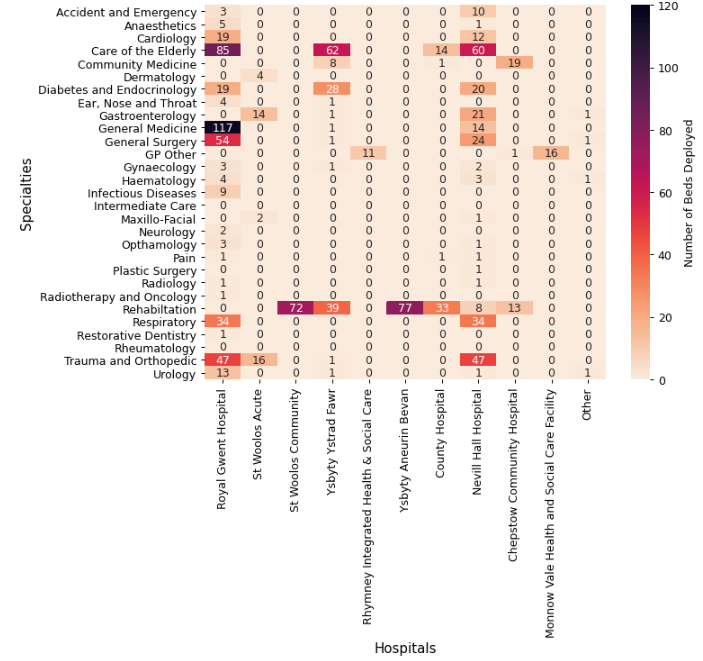
\includegraphics[width=\textwidth]{Chapters/Chapter5/Figures/2017STOC.png}
         \caption{2017 - 2018}
         \label{fig:stocexp2a}
     \end{subfigure}
\hfill
     \begin{subfigure}{0.8\textwidth}\ContinuedFloat
         \centering
         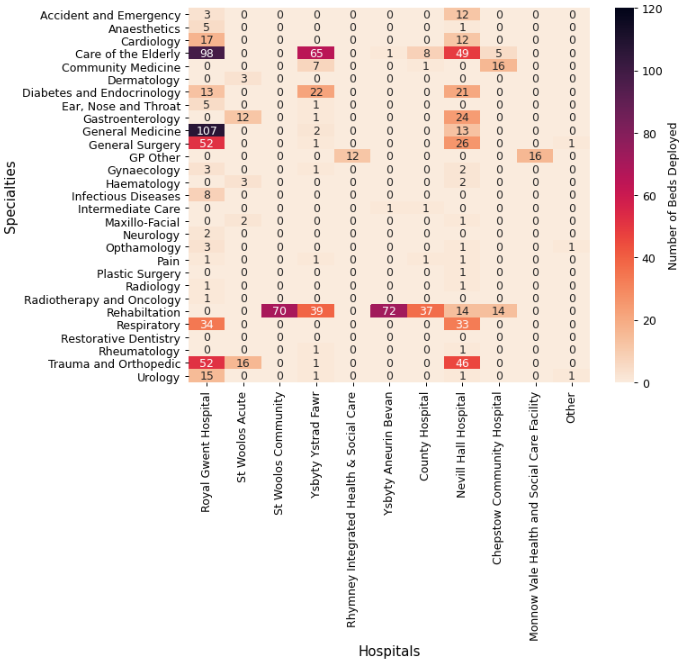
\includegraphics[width=\textwidth]{Chapters/Chapter5/Figures/2018STOC.png}
         \caption{2018 - 2019}
         \label{fig:stocexp2b}
     \end{subfigure}
     \end{figure}
\hfill
\begin{figure}\ContinuedFloat
     \begin{subfigure}{0.8\textwidth}
         \centering
         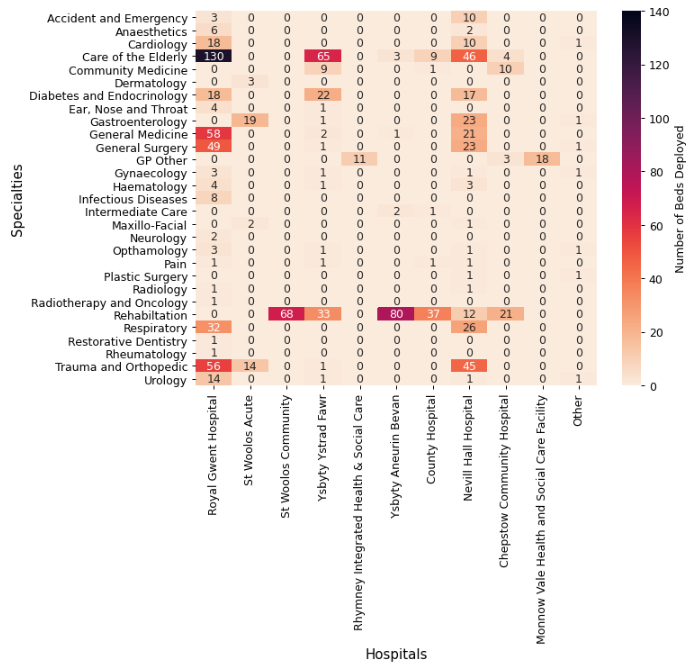
\includegraphics[width=\textwidth]{Chapters/Chapter5/Figures/2019STOC.png}
         \caption{2019 - 2020}
         \label{fig:stocexp2c}
     \end{subfigure}
        \caption{Heatmap of Bed Locations for Each Specialty Within Each Hospital by Year - Two-Stage Stochastic Results - Experiment 2 - Excel OpenSolver}
        \label{fig:stocexp2}
\end{figure}




\subsubsubsection{Test A}
Test A calculates the VSS to determine the benefit of using the stochastic solution over the deterministic solution. Table \ref{tab:eevdetstocresults2} displays the EEV, for each year. By fixing the deterministic variables, the stochastic nature of healthcare can be realised and the model can determine the additional number of beds that would be required if the deterministic values were used.


\begin{table}
    \centering
    \begin{tabular}{ccccccl}\toprule
 & \multirow{2}{*}{\textbf{Year}}& \multicolumn{2}{l}{\textbf{Total Beds}} & \multicolumn{2}{c}{\textbf{Total Staff}} & \multirow{2}{*}{\textbf{Objective Value ($\pounds$)}}\\ \cmidrule(lr){3-4} \cmidrule(lr){5-6}
&& xbed           & ubed          & xstaff         & ustaff         \\ \midrule
     \multirow{3}{*}{Deterministic} & 2017 - 2018 & 1031 & - &  594 & - & 1,000,612.28 =  EV$_{17-18}$ \\ 
      & 2018 - 2019 & 1015 & - & 591 & - & 993,114.92 =  EV$_{18-19}$ \\
      & 2019 - 2020 & 1010 & - & 594 & - & 996,035.28 =  EV$_{19-20}$\\ \midrule
     \multirow{3}{*}{Stochastic} & 2017 - 2018 & 1006 & 123 & 573 & 90 & 1,036,584.08 =  RP$_{17-18}$ \\ 
      & 2018 - 2019 & 986 & 133 & 573 & 96 & 1,030,014.36 =  RP$_{18-19}$ \\
      & 2019 - 2020 & 979 & 134 & 564 & 99 & 1,026,981.72 =  RP$_{19-20}$\\ \midrule    
     \multirow{3}{*}{Test A} & 2017 - 2018 & 1031 & 101 & 594 & 105 & 1,057,620.68 =  EEV$_{17-18}$ \\ 
      & 2018 - 2019 & 1015 & 100 & 591 & 105 &  1,051,293.68 =  EEV$_{18-19}$ \\
      & 2019 - 2020 & 1010 & 97 & 594 & 120 & 1,056,871.38 =  EEV$_{19-20}$\\ \bottomrule       
    \end{tabular}
    \caption{EEV, Deterministic and Two-Stage Stochastic Results - Experiment 2 - Excel OpenSolver}
    \label{tab:eevdetstocresults2}
\end{table}

The VSS ranges from between 1.95\% to 2.73\%, showing that the total cost is increasing by up to 2.73\% by implementing the deterministic solution.
\begin{align}
    \text{VSS}_{17-18} &= \text{EEV}_{17-18} - \text{RP}_{17-18} = \pounds21,03 6.60 (2.03\%)  \\
    \text{VSS}_{18-19} &= \text{EEV}_{18-19} - \text{RP}_{18-19} = \pounds21,279.32 (2.07\%)  \\
    \text{VSS}_{19-20} &= \text{EEV}_{19-20} - \text{RP}_{19-20} = \pounds29,889.66 (2.91\%)  
\end{align}

There are a number of reasons why the deterministic solution is considered poor. The model may be too optimistic on the randomness leading to insufficient beds and staff being deployed or the model could be planning the wrong beds and staff. This can be determined by calculating the LUSS and LUDS values.

\subsubsubsection{Test B}
The EESV is calculated by fixing the zero variables produced in the deterministic result and allowing the stochastic model to run. After performing the experiments, it was determined that the EESV is equal to the EEV in all cases (Table \ref{tab:eesveevdetstocresults2}).

\begin{table}[h!]
    \centering
    \begin{tabular}{ccccccl}\toprule
 & \multirow{2}{*}{\textbf{Year}}& \multicolumn{2}{l}{\textbf{Total Beds}} & \multicolumn{2}{c}{\textbf{Total Staff}} & \multirow{2}{*}{\textbf{Objective Value ($\pounds$)}}\\ \cmidrule(lr){3-4} \cmidrule(lr){5-6}
&& xbed           & ubed          & xstaff         & ustaff         \\ \midrule
     \multirow{3}{*}{Deterministic} & 2017 - 2018 & 1031 & - &  594 & - & 1,000,612.28 =  EV$_{17-18}$ \\ 
      & 2018 - 2019 & 1015 & - & 591 & - & 993,114.92 =  EV$_{18-19}$ \\
      & 2019 - 2020 & 1010 & - & 594 & - & 996,035.28 =  EV$_{19-20}$\\ \midrule
     \multirow{3}{*}{Stochastic} & 2017 - 2018 & 1006 & 123 & 573 & 90 & 1,036,584.08 =  RP$_{17-18}$ \\ 
      & 2018 - 2019 & 986 & 133 & 573 & 96 & 1,030,014.36 =  RP$_{18-19}$ \\
      & 2019 - 2020 & 979 & 134 & 564 & 99 & 1,026,981.72 =  RP$_{19-20}$\\ \midrule    
     \multirow{3}{*}{Test A} & 2017 - 2018 & 1031 & 101 & 594 & 105 & 1,057,620.68 =  EEV$_{17-18}$ \\ 
      & 2018 - 2019 & 1015 & 100 & 591 & 105 &  1,051,293.68 =  EEV$_{18-19}$ \\
      & 2019 - 2020 & 1010 & 97 & 594 & 120 & 1,056,871.38 =  EEV$_{19-20}$\\  \midrule  
     \multirow{3}{*}{Test B} &  2017 - 2018 & 1006 & 123 & 573 & 90 & 1,036,584.08 =    EESV$_{17-18}$ \\ 
      & 2018 - 2019 & 986 & 133 & 573 & 96 & 1,030,014.36 =   EESV$_{18-19}$ \\
      & 2019 - 2020 & 979 & 134 & 564 & 99 & 1,026,981.72 =  EESV$_{19-20}$\\ \bottomrule   
    \end{tabular}
    \caption{EESV, EEV, Deterministic and Two-Stage Stochastic Results - Experiment 2 - Excel OpenSolver}
    \label{tab:eesveevdetstocresults2}
\end{table}

The LUSS is calculated to be between $\pounds$0 for all three cases. The LUSS is equal to the RP and therefore corresponds to the perfect skeleton solution. This suggests that the variables selected by the deterministic solution are good.
%and $\pounds$29,889.66. Therefore, the LUSS is equal to the VSS and the stochastic programme chooses not to change the value of any of the remaining variables. For all three cases the following in therefore true, $EEV-EV \geq VSS = LUSS \geq 0$

\begin{align}
    \text{LUSS}_{17-18} &= \text{EESV}_{17-18} - \text{RP}_{17-18} = \pounds0   \\
    \text{LUSS}_{18-19} &= \text{EESV}_{18-19} - \text{RP}_{18-19} = \pounds0  \\
    \text{LUSS}_{19-20} &= \text{EESV}_{19-20} - \text{RP}_{19-20} = \pounds0
\end{align}

\subsubsubsection{Test C}
The final test involves taking the decision variables determined by deterministic solution and adding this as a minimum constraint. These results can be seen within Table \ref{tab:eiveesveevdetstocresults2}. 


\begin{table}[h!]
    \centering
    \begin{tabular}{ccccccl}\toprule
 & \multirow{2}{*}{\textbf{Year}}& \multicolumn{2}{l}{\textbf{Total Beds}} & \multicolumn{2}{c}{\textbf{Total Staff}} & \multirow{2}{*}{\textbf{Objective Value ($\pounds$)}}\\ \cmidrule(lr){3-4} \cmidrule(lr){5-6}
&& xbed           & ubed          & xstaff         & ustaff         \\ \midrule
     \multirow{3}{*}{Deterministic} & 2017 - 2018 & 1031 & - &  594 & - & 1,000,612.28 =  EV$_{17-18}$ \\ 
      & 2018 - 2019 & 1015 & - & 591 & - & 993,114.92 =  EV$_{18-19}$ \\
      & 2019 - 2020 & 1010 & - & 594 & - & 996,035.28 =  EV$_{19-20}$\\ \midrule
     \multirow{3}{*}{Stochastic} & 2017 - 2018 & 1006 & 123 & 573 & 90 & 1,036,584.08 =  RP$_{17-18}$ \\ 
      & 2018 - 2019 & 986 & 133 & 573 & 96 & 1,030,014.36 =  RP$_{18-19}$ \\
      & 2019 - 2020 & 979 & 134 & 564 & 99 & 1,026,981.72 =  RP$_{19-20}$\\ \midrule    
     \multirow{3}{*}{Test A} & 2017 - 2018 & 1031 & 101 & 594 & 105 & 1,057,620.68 =  EEV$_{17-18}$ \\ 
      & 2018 - 2019 & 1015 & 100 & 591 & 105 &  1,051,293.68 =  EEV$_{18-19}$ \\
      & 2019 - 2020 & 1010 & 97 & 594 & 120 & 1,056,871.38 =  EEV$_{19-20}$\\  \midrule    
     \multirow{3}{*}{Test B} &  2017 - 2018 & 1006 & 123 & 573 & 90 & 1,036,584.08 =    EESV$_{17-18}$ \\ 
      & 2018 - 2019 & 986 & 133 & 573 & 96 & 1,030,014.36 =   EESV$_{18-19}$ \\
      & 2019 - 2020 & 979 & 127 & 564 & 99 & 1,026,981.72 = EESV$_{19-20}$\\\midrule 
     \multirow{3}{*}{Test C} & 2017 - 2018 & 1047 & 85 & 594 & 81 & 1,053,935.22 =  EIV$_{17-18}$ \\ 
      & 2018 - 2019 & 1030 & 84 & 591 & 81 &  1,047,432.52 =  EIV$_{18-19}$ \\
      & 2019 - 2020 & 1033 & 74 & 594 & 78 & 1,050,205.36 =  EIV$_{19-20}$\\\bottomrule
    \end{tabular}
    \caption{EIV, EESV, EEV, Deterministic and Two-Stage Stochastic Results - Experiment 2 - Excel OpenSolver}
    \label{tab:eiveesveevdetstocresults2}
\end{table}

\begin{align}
    \text{LUDS}_{17-18} &= \text{EIV}_{17-18} - \text{RP}_{17-18} = \pounds17,351.14\\
    \text{LUDS}_{18-19} &= \text{EIV}_{18-19} - \text{RP}_{18-19} = \pounds17,418.16   \\
    \text{LUDS}_{19-20} &= \text{EIV}_{19-20} - \text{RP}_{19-20} = \pounds23,223.64 
\end{align}

Therefore, $EEV-EV \geq VSS \geq LUDS \geq 0$ is true. This result corresponds to partial upgradeability, where the deterministic results are are upgraded in first stage results by the stochastic model.

\subsubsubsection{Summary}
This section has analyses the bed and staffing requirements based on a year to year basis and determined where there is variation in the system. The largest VSS of 2.91\%, shows a potential saving of up to $\pounds$10,939,615.56 per year. As $LUSS=RP$, this shows that the deterministic does perform well but does not sufficiently deploy enough beds and staff. Therefore required wards and staff are deployed in the stochastic environment, at an additional cost.

Similar to the previous experiment, the deterministic solution did not perform well in a stochastic environment since insufficient beds and staff are deployed across all three years. This shows the deterministic model is too optimistic in terms of the demand.


\subsection{Python PuLP Results}\label{sec:pulpresults}
The optimisation package PuLP \cite{Mitchell2019} was used within Python to generate the deterministic and two-stage stochastic modelling results. PuLP using the CBC solver, provides the user with a number of parameters that can be changed. Within this model, the two following parameters are changed, with the rest remaining as their default.
\begin{itemize}
    \item maxSeconds
    \item fracGap
\end{itemize}

The `maxSeconds' determines the maximum run time for the solver, which to keep the results in comparison with the Microsoft Excel model, was set to 100 seconds. The `fracGap' determines the relative gap tolerance for the solver to stop, i.e., how close it is to the true value. This was set to a value of 0.01. If the results are not able to meet the `fracGap' criteria within the `maxSeconds', a non-optimal solution will be returned.

This section will perform the same experiments as Section \ref{ssec:opensolverresult}, to determine if there is a difference in the objective function, computational run time and locations of beds and staff.

\subsubsection{Experiment 1}
Recall experiment one where three years worth of data is utilised to determine the daily demand for beds and staff. Table \ref{tab:regionaldemands1} presents the regional demands which will be used to determine the daily bed requirements.


\subsubsubsection{Deterministic Model}
Using the first stage variables shown in Table \ref{tab:appstochpa}, a total number of 964 beds and 603 nurses were deployed. This therefore resulted in a daily cost of $\pounds$1,011,291.52.

Figure \ref{fig:pythondet1} displays the hospital speciality locations for all 1026 beds. The computational runtime of the optimisation programme was 1.75 seconds, showing the model performs efficiently.


\begin{figure}[h!]
    \centering
    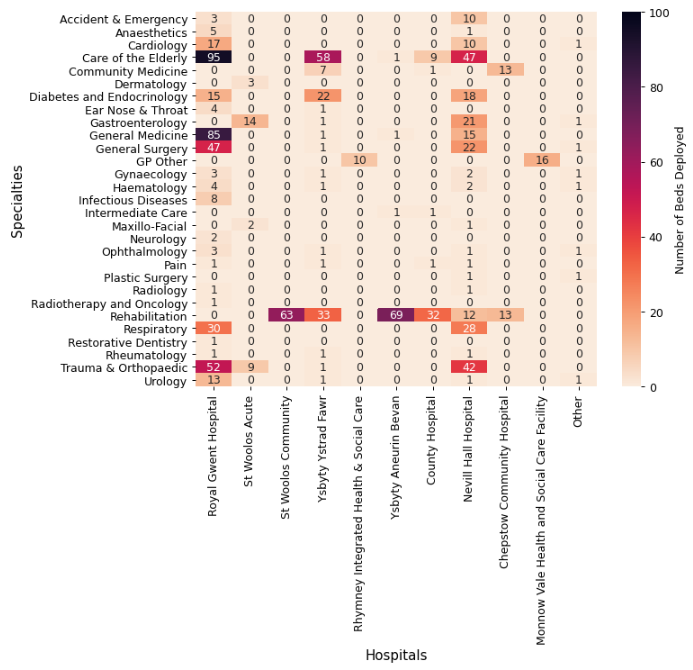
\includegraphics{Chapters/Chapter5/Figures/exdet.png}
    \caption{Heatmap of Bed Locations for Each Specialty Within Each Hospital - Deterministic Results - Python PuLP Solver}
    \label{fig:pythondet1}
\end{figure}

\subsubsubsection{Two-Stage Stochastic Model}
To determine the robustness of the model in a stochastic environment, the two-stage stochastic model with four scenarios was performed. Table \ref{tab:stochasticscenarios} which contains the four scenarios and their probability of occurring, in turn producing Tables \ref{tab:regionaldemandsexp2a} and Table \ref{tab:regionaldemandsexp2b}.

\begin{table}[h!]
    \centering
    \begin{tabular}{@{}cc@{}}\toprule
       \textbf{Scenario}  &\textbf{Probability}  \\\midrule
       Demand Increases by 5\% & 25\% \\ 
       Demand Increases by 10\% & 25\% \\
       Demand Decreases by 5\% & 25\% \\ 
       Demand Decreases by 10\% & 25\% \\\bottomrule
    \end{tabular}
    \caption{Four Scenarios for the Two-Stage Stochastic Model}
    \label{tab:stochasticscenarios}
\end{table}

The two stage stochastic model produced an objective function of $\pounds$1,051,271.44, increasing by 3.95\% compared to the deterministic solution. This required a 968 beds to be deployed in the first stage, with an additional 165 beds required in the second stage. A minimum number of 668 nursing staff are required over a 24 hour period.

\begin{table}[h!]
    \centering
    \begin{tabular}{cccccl}\toprule
 & \multicolumn{2}{l}{\textbf{Total Beds}} & \multicolumn{2}{c}{\textbf{Total Staff}} & \multirow{2}{*}{\textbf{Objective Value ($\pounds$)}}\\ \cmidrule(lr){2-3} \cmidrule(lr){4-5}
 & xbed           & ubed          & xstaff         & ustaff         \\ \midrule
      Deterministic & 1026 & - &  621 & - & 1,011,291.52 =  EV \\ \midrule
      Stochastic & 968  & 165 &  575 & 93 &1,051,271.44 = RP\\  \bottomrule
    \end{tabular}
    \caption{Deterministic and Two-Stage Stochastic Results - Experiment 1 - Python PuLP}
    \label{tab:dettwostageresults1python}
\end{table}

Figure \ref{fig:pythonstocheatmap} presents the number of beds for each specialty location within the healthboard.


\begin{figure}
    \centering
    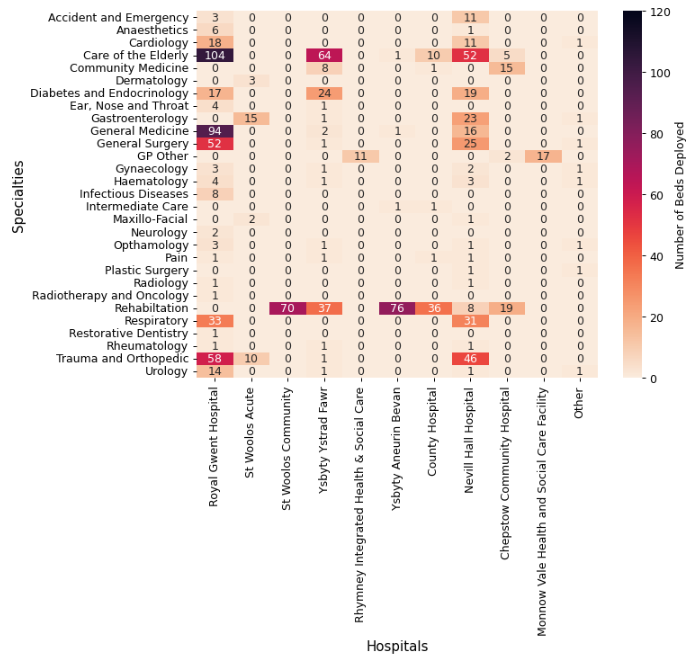
\includegraphics{Chapters/Chapter5/Figures/PythonStoc.png}
    \caption{Heatmap of Bed Locations for Each Specialty within Each Hospital - Two-Stage Stochastic Results - Experiment 1 - Python PuLP Solver}
    \label{fig:pythonstocheatmap}
\end{figure}


\subsubsubsection{Test A}
The deterministic results of 1026 beds and 621 staff were fixed as the first stage variables into the two-stage stochastic programme.

The EEV was calculated to be $\pounds$1,070,453.74, which in turn produces a VSS of 2.1\% (Table \ref{tab:eevdettwostageresults1python}). 
\begin{equation}
    VSS = 1,051,271.44 - 1,029,605.24 = 21,666.20
\end{equation}

This value equates to a saving of $\pounds$21,666.20 per day. If used over a year period, this would in total save a potential of $\pounds$7,908,163. This result demonstrates the benefit of using the two-stage stochastic model over the deterministic model. The two-stage stochastic model leads to more realistic and robust decision making.

\begin{table}[h!]
    \centering
    \begin{tabular}{cccccl}\toprule
 & \multicolumn{2}{l}{\textbf{Total Beds}} & \multicolumn{2}{c}{\textbf{Total Staff}} & \multirow{2}{*}{\textbf{Objective Value ($\pounds$)}}\\ \cmidrule(lr){2-3} \cmidrule(lr){4-5}
 & xbed           & ubed          & xstaff         & ustaff         \\ \midrule     
      Deterministic & 1026 & - &  621 & - & 1,011,291.52 =  EV \\ \midrule
      Stochastic & 968  & 165 &  575 & 93 &1,051,271.44 = RP\\\midrule
      Test A & 1026 & 101 & 621 & 111 & 1,070,453.74 = EEV \\\bottomrule
    \end{tabular}
    \caption{EEV, Deterministic and Two-Stage Stochastic Results - Experiment 1 - Python PuLP}
    \label{tab:eevdettwostageresults1python}
\end{table}
To gain further understanding on the VSS and why the deterministic solution does not perform as expected, the following two tests can be performed.

\subsubsubsection{Test B}
The decision variables which were determined in the deterministic solution with the value of zero, were fixed in the first stage of the stochastic solution. This produced an objective function value of $\pounds$1,051,271.44 (Table \ref{tab:eesveevdettwostageresults1python}).

\begin{table}[h!]
    \centering
    \begin{tabular}{cccccl}\toprule
 & \multicolumn{2}{l}{\textbf{Total Beds}} & \multicolumn{2}{c}{\textbf{Total Staff}} & \multirow{2}{*}{\textbf{Objective Value ($\pounds$)}}\\ \cmidrule(lr){2-3} \cmidrule(lr){4-5}
 & xbed           & ubed          & xstaff         & ustaff         \\ \midrule
      Deterministic & 1026 & - &  621 & - & 1,011,291.52 =  EV \\ \midrule
      Stochastic & 968  & 165 &  575 & 93 &1,051,271.44 = RP\\\midrule
      Test A & 1026 & 101 & 621 & 111 & 1,070,453.74 = EEV \\\midrule
      Test B & 1026 & 101 & 621 & 111 & 1,070,453.74 = EESV \\\bottomrule
    \end{tabular}
    \caption{EESV, EEV, Deterministic and Two-Stage Stochastic Results - Experiment 1 - Python PuLP}
    \label{tab:eesveevdettwostageresults1python}
\end{table}
 Since the EESV value is greater than RP, the LUSS value is calculated to be $\pounds$21,666.20:
 \begin{equation}
     LUSS = 1,051,271.44 - 1,029,605.24 = 21,666.20
 \end{equation}
The LUSS measures the loss by deploying beds and staff only in locations determined by the deterministic solution. The model reacts by choosing not to change the value of the remaining variables, and wards opened in the deterministic solution remain the same. This results in the LUSS and VSS values being equal.

\subsubsubsection{Test C}
The third and final test uses the values found within the deterministic and sets these as a minimum constraints to be met. This checks the upgradability of the resources in a stochastic environment. The EIV value was calculated to be $\pounds$1,065,666.86 (Table \ref{tab:eiveevdettwostageresults1python}). A EIV value was produced equal to the EEV, and therefore the LUDS less than the VSS. This shows that the model is partially upgradeable and the deterministic results are upgraded in the first stage of the stochastic model.
\begin{equation}
    LUDS =  1,065,666.86 - 1,051,271.44 = 14,395.42
\end{equation}


\begin{table}[h!]
    \centering
    \begin{tabular}{cccccl}\toprule
 & \multicolumn{2}{l}{\textbf{Total Beds}} & \multicolumn{2}{c}{\textbf{Total Staff}} & \multirow{2}{*}{\textbf{Objective Value ($\pounds$)}}\\ \cmidrule(lr){2-3} \cmidrule(lr){4-5}
 & xbed           & ubed          & xstaff         & ustaff         \\ \midrule
     Deterministic & 1026 & - &  621 & - & 1,011,291.52 =  EV \\ \midrule
      Stochastic& 968  & 165 &  575 & 93 &1,051,271.44 = RP\\\midrule
      Test A & 1026 & 101 & 621 & 111 & 1,070,453.74 = EEV \\\midrule
      Test B & 1026 & 101 & 621 & 111 & 1,070,453.74 = EESV \\\midrule
      Test C & 1042 & 86 &  621  & 78 &  1,065,666.86 = EIV\\\bottomrule
    \end{tabular}
    \caption{EIV, EESV, EEV, Deterministic and Two-Stage Stochastic Results - Experiment 1 - Python PuLP}
    \label{tab:eiveevdettwostageresults1python}
\end{table}
\subsubsubsection{Summary}
This section has analysed the number of beds and staff to be deployed within the healthboard for three years worth of data. The VSS has shown there is a 2.1\% saving, equating to $\pounds$21,666.20 saved per day. Across all three years of data, if implemented has the potential to save approximately $\pounds$22.7 million. Although using data generated through NHS Scotland records, it highlights the importance of using the stochastic solution over the deterministic model and the savings that ABUHB could make. 

\subsubsection{Experiment 2}
The second experiment analyses the three years worth of data on a year to year basis to determine if demand fluctuates based on year. Tables \ref{tab:regionaldemandsexp2a} and \ref{tab:regionaldemandsexp2b} contain the regional demands for each of the three years of patient admissions. Tables \ref{tab:appdetermpa} and \ref{tab:appstochpa} contain the deterministic and two-stage stochastic parameters respectively. 

\subsubsubsection{Deterministic Model}
The deterministic model utilised the average daily demands as the minimum number of beds that are required to be met, and then calculates the required number of staff to be deployed. Table \ref{tab:detresultspy2} presents the number of beds and staff required for each of the three years.

\begin{table}[h!]
    \centering
    \begin{tabular}{ccccccl}\toprule
 & \multirow{2}{*}{\textbf{Year}}& \multicolumn{2}{l}{\textbf{Total Beds}} & \multicolumn{2}{c}{\textbf{Total Staff}} & \multirow{2}{*}{\textbf{Objective Value ($\pounds$)}}\\ \cmidrule(lr){3-4} \cmidrule(lr){5-6}
&& xbed           & ubed          & xstaff         & ustaff         \\ \midrule
     \multirow{3}{*}{Deterministic} & 2017 - 2018 & 1031 & - &  594 & - & 1,000,612,28 =  EV$_{17-18}$ \\ 
      & 2018 - 2019 & 1015 & - & 591 & - & 993,114.92 =  EV$_{18-19}$ \\
      & 2019 - 2020 & 1010 & - & 594 & - & 996,035.28 =  EV$_{19-20}$\\ \bottomrule
    \end{tabular}
    \caption{Deterministic Results - Experiment 2 - Python PuLP}
    \label{tab:detresultspy2}
\end{table}

The results show that the year 2017 - 2018 requires the largest demand of beds and staff and therefore has the largest associated EV value. Figure \ref{fig:detexppy2} displays each of the three heatmaps showing the number of beds to deploy for each specialty each year. 



\begin{figure}
     \centering
     \begin{subfigure}[h!]{0.8\textwidth}
         \centering
         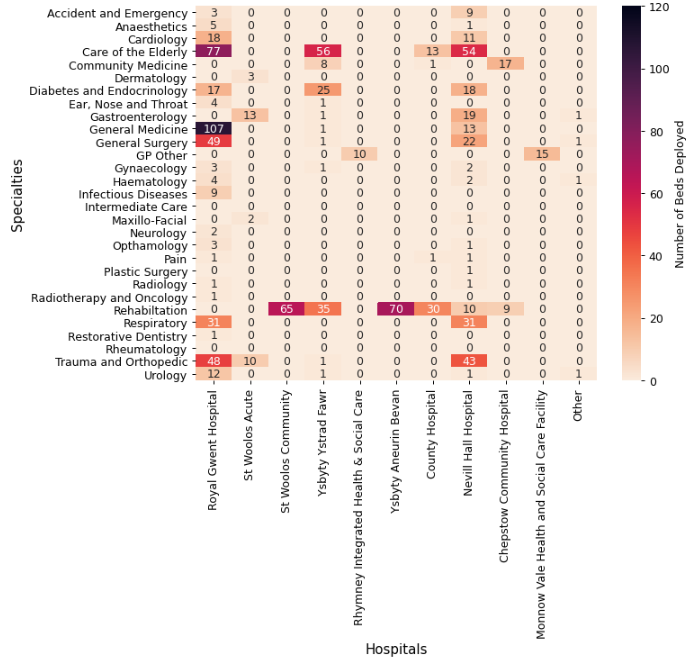
\includegraphics[width=\textwidth]{Chapters/Chapter5/Figures/2017DET.png}
         \caption{2017 - 2018}
         \label{fig:detexppy2a}
     \end{subfigure}
\hfill
     \begin{subfigure}{0.8\textwidth}
         \centering
         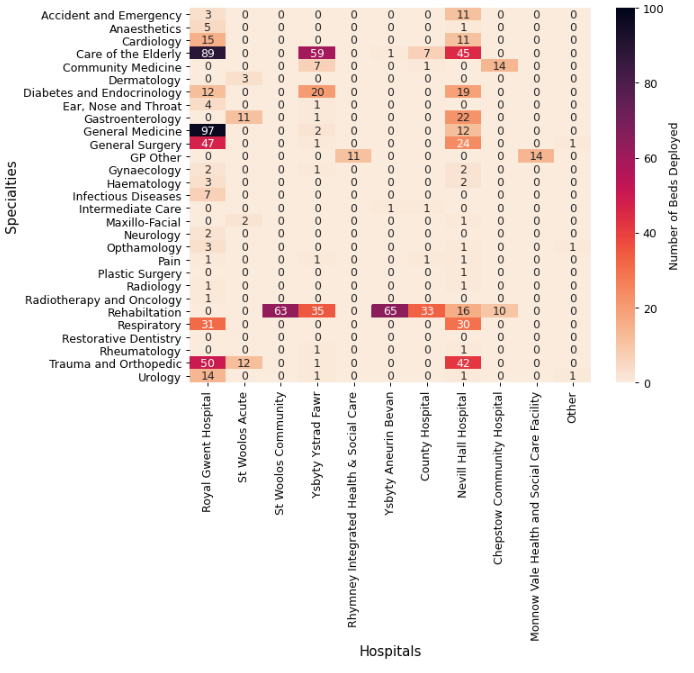
\includegraphics[width=\textwidth]{Chapters/Chapter5/Figures/2018DET.png}
         \caption{2018 - 2019}
         \label{fig:detexppy2b}
     \end{subfigure}
     \end{figure}
\hfill
\begin{figure}\ContinuedFloat
     \begin{subfigure}{0.8\textwidth}
         \centering
         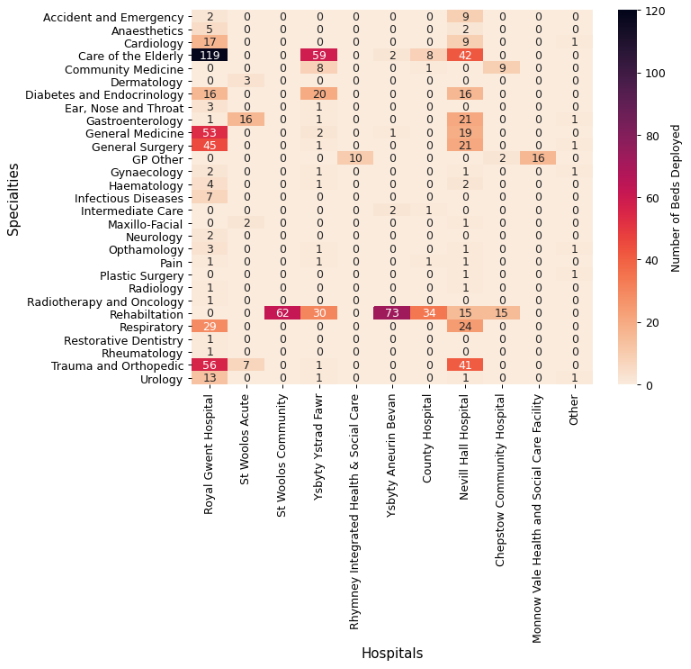
\includegraphics[width=\textwidth]{Chapters/Chapter5/Figures/2019DET.png}
         \caption{2019 - 2020}
         \label{fig:detexppy2c}
     \end{subfigure}
        \caption{Heatmap of Bed Locations for Each Specialty Within Each Hospital by Year - Deterministic Results - Experiment 2 - Python PuLP}
        \label{fig:detexppy2}
\end{figure}

\subsubsubsection{Two-Stage Stochastic Model}
The two-stage stochastic model considered four scenarios which have been previously discussed. These scenarios have an average of the deterministic demand, but demonstrates the stochastic nature of healthcare. Table \ref{tab:detstocresultspy2} displays the two-stage stochastic results in comparison to the deterministic results. In all three cases, fewer first stage beds are deployed, resulting in a larger number of second stage beds being deployed, with a higher associated cost. This trend is also applicable to the staffing. 

\begin{table}[h!]
    \centering
    \begin{tabular}{ccccccl}\toprule
 & \multirow{2}{*}{\textbf{Year}}& \multicolumn{2}{l}{\textbf{Total Beds}} & \multicolumn{2}{c}{\textbf{Total Staff}} & \multirow{2}{*}{\textbf{Objective Value ($\pounds$)}}\\ \cmidrule(lr){3-4} \cmidrule(lr){5-6}
&& xbed           & ubed          & xstaff         & ustaff         \\ \midrule
     \multirow{3}{*}{Deterministic} & 2017 - 2018 & 1031 & - &  594 & - & 1,000,612,28 =  EV$_{17-18}$ \\ 
      & 2018 - 2019 & 1015 & - & 591 & - & 993,114.92 =  EV$_{18-19}$ \\
      & 2019 - 2020 & 1010 & - & 594 & - & 996,035.28 =  EV$_{19-20}$\\\midrule
     \multirow{3}{*}{Stochastic} & 2017 - 2018 & 951 & 189 & 528 & 144 & 1,034,194.64 =  RP$_{17-18}$ \\ 
      & 2018 - 2019 & 949 & 171 & 534 & 123 & 1,022,665.28 =  RP$_{18-19}$ \\
      & 2019 - 2020 & 950 & 162 & 531 & 117 & 1,020,711.04 =  RP$_{19-20}$\\ \bottomrule      
    \end{tabular}
    \caption{Deterministic and Two-Stage Stochastic Results - Experiment 2 - Python PuLP}
    \label{tab:detstocresultspy2}
\end{table}

To determine the location and differences between specialty bed locations, three heatmaps (Figures \ref{fig:stocexppy2a}, \ref{fig:stocexppy2b} and \ref{fig:stocexppy2c}), are presented. RGH, YYF, YAB and NHH are only four hospital locations in which the number of specialties open each year changes. For example, in 2017 - 2018, RGH requires one restorative dentistry bed for the over 65's, which the model then suggests to open zero in 2018 - 2019, before reopening the one bed in 2019 - 2020.  For the model to be successfully implemented, it would require yearly monitoring and updates of specialty locations. In practice this could prove impractical to move medical supplies between hospitals each year.


\begin{figure}
     \centering
     \begin{subfigure}[h!]{0.8\textwidth}
         \centering
         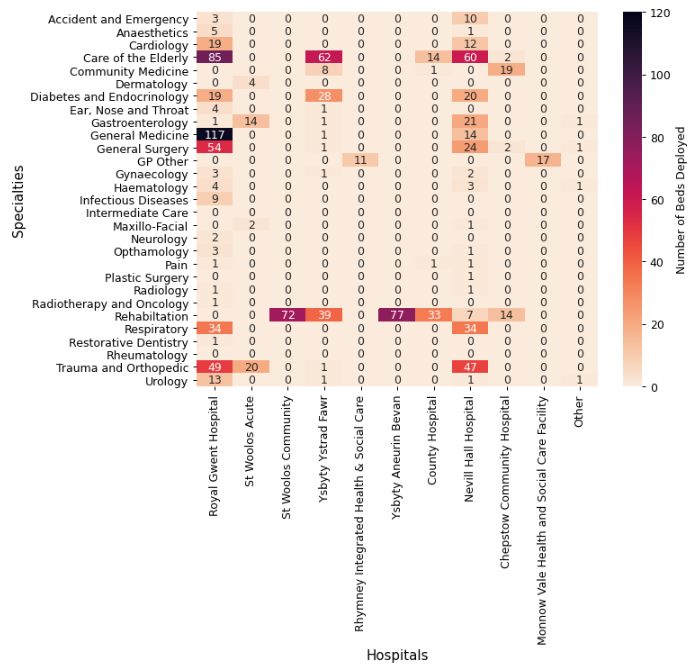
\includegraphics[width=\textwidth]{Chapters/Chapter5/Figures/python2017stoch.png}
         \caption{2017 - 2018}
         \label{fig:stocexppy2a}
     \end{subfigure}
\hfill
     \begin{subfigure}{0.8\textwidth}\ContinuedFloat
         \centering
         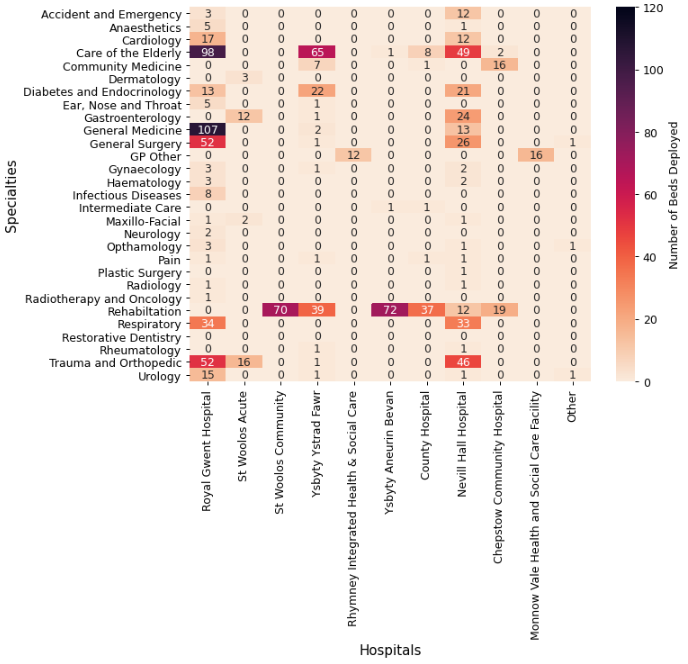
\includegraphics[width=\textwidth]{Chapters/Chapter5/Figures/python2018stoch.png}
         \caption{2018 - 2019}
         \label{fig:stocexppy2b}
     \end{subfigure}
     \end{figure}
\hfill
\begin{figure}\ContinuedFloat
     \begin{subfigure}{0.8\textwidth}
         \centering
         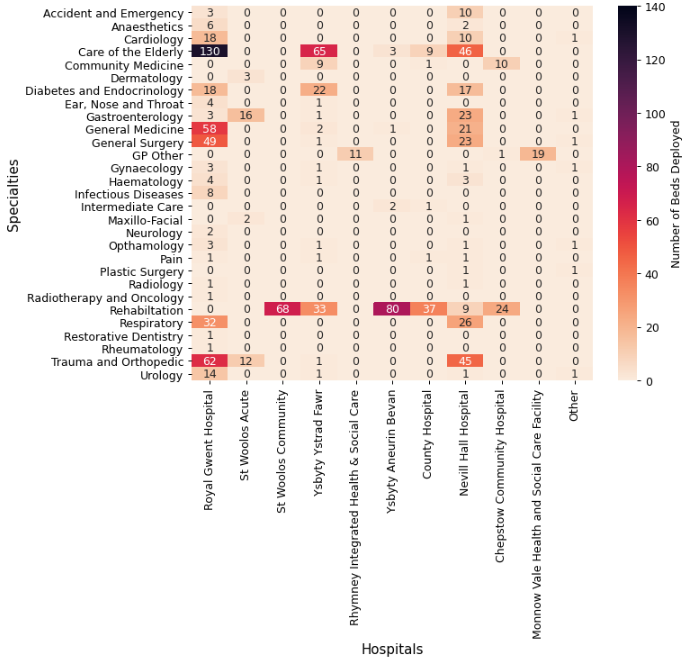
\includegraphics[width=\textwidth]{Chapters/Chapter5/Figures/python2019stoch.png}
         \caption{2019 - 2020}
         \label{fig:stocexppy2c}
     \end{subfigure}
        \caption{Heatmap of Bed Locations for Each Specialty Within Each Hospital by Year - Two-Stage Stochastic Results - Experiment 2 - Python PuLP}
        \label{fig:stocexppy2}
\end{figure}

\subsubsubsection{Test A}
The VSS is calculated to show the benefit of using the stochastic solution compared to the deterministic solution, and the financial implications for this. Table \ref{tab:eevdetstocresultspy2} presents the EEV for the three years. If the healthboard were to plan using the deterministic results, the EEV shows the maximum additional beds and staff that would be required.

\begin{table}[h!]
    \centering
    \begin{tabular}{ccccccl}\toprule
 & \multirow{2}{*}{\textbf{Year}}& \multicolumn{2}{l}{\textbf{Total Beds}} & \multicolumn{2}{c}{\textbf{Total Staff}} & \multirow{2}{*}{\textbf{Objective Value ($\pounds$)}}\\ \cmidrule(lr){3-4} \cmidrule(lr){5-6}
&& xbed           & ubed          & xstaff         & ustaff         \\ \midrule
     \multirow{3}{*}{Deterministic} & 2017 - 2018 & 1031 & - &  594 & - & 1,000,612,28 =  EV$_{17-18}$ \\ 
      & 2018 - 2019 & 1015 & - & 591 & - & 993,114.92 =  EV$_{18-19}$ \\
      & 2019 - 2020 & 1010 & - & 594 & - & 996,035.28 =  EV$_{19-20}$\\\midrule
     \multirow{3}{*}{Stochastic} & 2017 - 2018 & 951 & 189 & 528 & 144 & 1,034,194.64 =  RP$_{17-18}$ \\ 
      & 2018 - 2019 & 949 & 171 & 534 & 123 & 1,022,665.28 =  RP$_{18-19}$ \\
      & 2019 - 2020 & 950 & 162 & 531 & 117 & 1,020,711.04 =  RP$_{19-20}$\\ \midrule
      \multirow{3}{*}{Test A} & 2017 - 2018 &1031 & 101 & 594 & 105 & 1,057,620.68 = EEV$_{17-18}$\\
      & 2018 - 2019 &1015 & 100 & 591 & 105 & 1,051,293.68 = EEV$_{18-19}$\\
      & 2019 - 2020 &1010 & 97 & 594 & 120 & 1,056,871.38 = EEV$_{19-20}$\\\bottomrule      
    \end{tabular}
    \caption{EEV, Deterministic and Two-Stage Stochastic Results - Experiment 2 - Python PuLP}
    \label{tab:eevdetstocresultspy2}
\end{table}

The VSS ranges from 2.27\% to 3.54\% which shows the value of using the stochastic solution to plan beds and staff for the elderly population.

\begin{align}
    \text{VSS}_{17-18} &= \text{EEV}_{17-18} - \text{RP}_{17-18} = \pounds23,426.04 (2.27\%)  \\
    \text{VSS}_{18-19} &= \text{EEV}_{18-19} - \text{RP}_{18-19} = \pounds28,628.40 (2.8\%)  \\
    \text{VSS}_{19-20} &= \text{EEV}_{19-20} - \text{RP}_{19-20} = \pounds36,169.34 (3.54\%)  
\end{align}

To ascertain why the deterministic solution plans a smaller number of beds, the LUSS and LUDS values can be calculated. This determines whether since the model does not have any randomness, under estimates the exact number of beds required or whether the wrong locations of beds are planned. 

\subsubsubsection{Test B}
The decision variables of value zero that were identified in the deterministic solution were fixed, and the model was run to determine if the correct deterministic values were selected. Table \ref{tab:eesveevdetstocresultspy2} shows that EESV is greater the RP in all cases, and smaller than the EEV.
Therefore the following is true:
\begin{equation}
    RP \leq EESV \leq EEV 
\end{equation}
\begin{equation}
    EEV - EV \geq VSS \geq LUSS \geq 0
\end{equation}

The LUSS ranges from $\pounds$551.08 to $\pounds$3,898.36, which is much smaller than the VSS value. This suggests the deterministic solution deploys a small number of beds and staff to the wrong location.

\begin{align}
    \text{LUSS}_{17-18} &= \text{EEV}_{17-18} - \text{RP}_{17-18} = \pounds352.90  \\
    \text{LUSS}_{18-19} &= \text{EEV}_{18-19} - \text{RP}_{18-19} = \pounds1,508.34  \\
    \text{LUSS}_{19-20} &= \text{EEV}_{19-20} - \text{RP}_{19-20} = \pounds5,837.22
\end{align}

\begin{table}[h!]
    \centering
    \begin{tabular}{ccccccl}\toprule
 & \multirow{2}{*}{\textbf{Year}}& \multicolumn{2}{l}{\textbf{Total Beds}} & \multicolumn{2}{c}{\textbf{Total Staff}} & \multirow{2}{*}{\textbf{Objective Value ($\pounds$)}}\\ \cmidrule(lr){3-4} \cmidrule(lr){5-6}
&& xbed           & ubed          & xstaff         & ustaff         \\ \midrule
     \multirow{3}{*}{Deterministic} & 2017 - 2018 & 1031 & - &  594 & - & 1,000,612,28 =  EV$_{17-18}$ \\ 
      & 2018 - 2019 & 1015 & - & 591 & - & 993,114.92 =  EV$_{18-19}$ \\
      & 2019 - 2020 & 1010 & - & 594 & - & 996,035.28 =  EV$_{19-20}$\\\midrule
     \multirow{3}{*}{Stochastic} & 2017 - 2018 & 951 & 189 & 528 & 144 & 1,034,194.64 =  RP$_{17-18}$ \\ 
      & 2018 - 2019 & 949 & 171 & 534 & 123 & 1,022,665.28 =  RP$_{18-19}$ \\
      & 2019 - 2020 & 950 & 162 & 531 & 117 & 1,020,711.04 =  RP$_{19-20}$\\ \midrule
      \multirow{3}{*}{Test A} & 2017 - 2018 &1031 & 101 & 594 & 105 & 1,057,620.68 = EEV$_{17-18}$\\
      & 2018 - 2019 &1015 & 100 & 591 & 105 & 1,051,293.68 = EEV$_{18-19}$\\
      & 2019 - 2020 &1010 & 97 & 594 & 120 & 1,056,871.38 = EEV$_{19-20}$\\\midrule
      \multirow{3}{*}{Test B} & 2017 - 2018 &960 & 180 & 525 & 127 & 1,034,547.54 = EESV$_{17-18}$\\
      & 2018 - 2019 &949 & 171 & 534 & 123 & 1,024,173.62 = EESV$_{18-19}$\\
      & 2019 - 2020 &949 & 166 & 538 & 120 & 1,026,548.26 = EESV$_{19-20}$\\\bottomrule      
    \end{tabular}
    \caption{EESV, EEV, Deterministic and Two-Stage Stochastic Results - Experiment 2 - Python PuLP}
    \label{tab:eesveevdetstocresultspy2}
\end{table}

\subsubsubsection{Test C}
The final investigates the upgradeability of the deterministic solution by setting the decision variables as a constraint for the stochastic as a minimum number to be met. The LUDS can then be calculated as follows:

\begin{align}
     \text{LUDS}_{17-18} &= \text{EIV}_{17-18} - \text{RP}_{17-18} = \pounds19,740.58   \\
    \text{LUDS}_{18-19} &= \text{EIV}_{18-19} - \text{RP}_{18-19} = \pounds24,767.24   \\
    \text{LUDS}_{19-20} &= \text{EIV}_{19-20} - \text{RP}_{19-20} = \pounds29,494.32
\end{align}

Since the LUDS values are all less than the VSS, this shows there is partial-upgradeability (Table \ref{tab:eiveesveevdetstocresultspy2}).

\begin{table}[h!]
    \centering
    \begin{tabular}{ccccccl}\toprule
 & \multirow{2}{*}{\textbf{Year}}& \multicolumn{2}{l}{\textbf{Total Beds}} & \multicolumn{2}{c}{\textbf{Total Staff}} & \multirow{2}{*}{\textbf{Objective Value ($\pounds$)}}\\ \cmidrule(lr){3-4} \cmidrule(lr){5-6}
&& xbed           & ubed          & xstaff         & ustaff         \\ \midrule
     \multirow{3}{*}{Deterministic} & 2017 - 2018 & 1031 & - &  594 & - & 1,000,612,28 =  EV$_{17-18}$ \\ 
      & 2018 - 2019 & 1015 & - & 591 & - & 993,114.92 =  EV$_{18-19}$ \\
      & 2019 - 2020 & 1010 & - & 594 & - & 996,035.28 =  EV$_{19-20}$\\\midrule
     \multirow{3}{*}{Stochastic} & 2017 - 2018 & 951 & 189 & 528 & 144 & 1,034,194.64 =  RP$_{17-18}$ \\ 
      & 2018 - 2019 & 949 & 171 & 534 & 123 & 1,022,665.28 =  RP$_{18-19}$ \\
      & 2019 - 2020 & 950 & 162 & 531 & 117 & 1,020,711.04 =  RP$_{19-20}$\\ \midrule
      \multirow{3}{*}{Test A} & 2017 - 2018 &1031 & 101 & 594 & 105 & 1,057,620.68 = EEV$_{17-18}$\\
      & 2018 - 2019 &1015 & 100 & 591 & 105 & 1,051,293.68 = EEV$_{18-19}$\\
      & 2019 - 2020 &1010 & 97 & 594 & 120 & 1,056,871.38 = EEV$_{19-20}$\\\midrule
      \multirow{3}{*}{Test B} & 2017 - 2018 &960 & 180 & 525 & 127 & 1,034,547.54 = EESV$_{17-18}$\\
      & 2018 - 2019 &949 & 171 & 534 & 123 & 1,024,173.62 = EESV$_{18-19}$\\
      & 2019 - 2020 &949 & 166 & 538 & 120 & 1,026,548.26 = EESV$_{19-20}$\\\midrule
       \multirow{3}{*}{Test C}& 2017 - 2018 &1047 & 85 & 594 & 84 & 1,053,935.22 = EIV$_{17-18}$\\
      & 2018 - 2019 &1030 & 84 & 591 & 81 & 1,047,432.52 = EIV$_{18-19}$\\
      & 2019 - 2020 &1033 & 74 & 594 & 78 & 1,050,205.36 = EIV$_{19-20}$\\\bottomrule      
    \end{tabular}
    \caption{EIV, EESV, EEV, Deterministic and Two-Stage Stochastic Results - Experiment 2 - Python PuLP}
    \label{tab:eiveesveevdetstocresultspy2}
\end{table}

\subsubsubsection{Summary}
This section has demonstrated the use of the Python package PuLP to determine the most efficient way to organise specialties and staff within ABUHB on a year to year basis. The largest VSS of 3.54\% determine a potential saving of up to $\pounds$13,237,978.44 per year. As the LUSS is always greater than zero, this demonstrates that the deterministic model selects the wrong choice of beds and staff.

\subsection{Excel OpenSolver and Python PuLP Comparisons}
Microsoft Excel OpenSolver and Python PuLP are two optimisation tools generated for this research. Due to the nature of how the packages are built, tolerance levels and maximum run times, small differences in the results may occur.

The deterministic model, whether performed in Excel or Python, always generated the same objective value function. Similarly, the VSS result also always produced the same value in the two models. There was a small difference between the models for the stochastic programme, with the largest difference being 0.1\% in Experiment 1 and 0.73\% in Experiment 2. This is due to the parameters and random seeds within Python. Since the difference is small, it does not make a large impact on overall cost and bed planning. In both the Excel and Python models, the two-stage stochastic solution had a longer computational time when compared to the deterministic.

Table \ref{tab:vsscomparisons} presents the Excel and Python VSS results per year and the total savings if implemented over the three years.

\begin{table}[h!]
    \centering
    \begin{tabular}{ccccc}\toprule
    & \multicolumn{2}{c}{\textbf{Experiment 1}}& \multicolumn{2}{c}{\textbf{Experiment 2}} \\
         & \textbf{Excel} & \textbf{Python}  & \textbf{Excel} & \textbf{Python} \\\midrule
         Year 1& $\pounds$7,681,877.60 & $\pounds$7,908,163 & $\pounds$7,678,359.00&$\pounds$8,550,504.60 \\
         Year 2& $\pounds$7,681,877.60  & $\pounds$7,908,163&$\pounds$7,766,951.80 &$\pounds$10,449,366.00\\
         Year 3& $\pounds$7,702,923.84  &$\pounds$7,929,829.20 &  $\pounds$10,939,615.56 &$\pounds$13,237,978.40\\\midrule
        Total Saving & $\pounds$23,066,679.04 & $\pounds$23,746,155.20&$\pounds$25,628,609.86&   $\pounds$32,237,849.00\\\bottomrule
    \end{tabular}
    \caption{VSS Comparisons comparing Experiment 1 to Experiment 2 - Year 3 is a leap year and therefore contains 366 days which accounts for the increase in savings}
    \label{tab:vsscomparisons}
\end{table}

The results highlight the importance to plan on a year to year time frame, rather than to plan for long scale horizons, with potential savings in the region of two times.

This section has discussed the research aim, `How best can specialties be organised among a network of hospitals to ensure staffing and bed costs are minimised'. The heatmaps produced visualise the number of beds to locate across different specialties in order to minimise costs. The models also determine the number of staff to deploy based on the number of beds. These models work under the assumption of current hospital locations, where a hospital cannot open wards if they do not have the resources for these specialities. The models perform by deploying beds to the cheapest locations first, determining the trade off between different combinations. Traditionally, ABUHB has planned on averages (deterministic solution), using historic data to determine the locality and quantity of these beds. By implementing a two-stage stochastic model, with different levels of demands, provides savings for the NHS from approximately 2\% per day. This saving has the potential to impact patient care by reallocating this money to additional resources, more staff training or improving community care schemes to reduce the pressures on hospitals.

\section{Linking Paradigms}\label{sec:linking}
One of the four research aims is to determine `how can linking predictive and prescriptive analytics increase the reliability of the models?'. This section aims to link the CART results with deterministic and two-stage stochastic models together to ensure the results are consistent. Two methods will be explored, firstly by using each end node and determining the number of patients of each specialty and hospital using the average LOS from each end node. The second method will take each end node and the specific LOS for each specialty and hospital within the node. These will then be summed together to form the D$_{s,r}$ parameter. These two methods will be run on both the regression and the classification trees, using the Microsoft Excel implementation. The results will be compared on a year to year basis, as well as a three year range. Similar to previous experiments, the models will be run with a maximum run time of 100 seconds and a tolerance of 0.01\%. The deterministic and two-stage stochastic models will be used to calculated the VSS. The demands utilised within this section and the resulting heatmaps can be seen within Appendix \ref{app:linkeddemands}.

\subsection{Regression Tree and Average LOS}
The first method utilises the regression tree generated in Section \ref{sec:regressiontrees}, Figure \ref{fig:finalregtree}. This tree generated 30 leaf nodes, and therefore 30 patient groupings. For each node, the demand can be calculated using the Average LOS determined by the node. Using Equation \eqref{eq:treedemand1}, the average demand can be calculated:

\begin{equation}\label{eq:treedemand1}
        D_{s,r} = \sum\limits_{h \in r} D_{s,h} = \frac{\text{Number of Patients}_{s,h}*\text{Node Average LOS}}{1096}
\end{equation}

Table \ref{tab:Node2Regression} displays the process of determining the average bed demand for node 2. Node 2 is the second left leaf node on Figure \ref{sec:regressiontrees}, where a patient falls under the following eleven criterion:
\begin{enumerate}
    \item Admission method $\neq$ Other - transferred from another hospital
    \item Admission method $\neq$ Elective - waiting list
    \item Admission method $\neq$ Elective - booked
    \item Specialty $\neq$ Accident \& Emergency
    \item Admission method $\neq$ Elective - planned
    \item Hospital $\neq$ Ysbyty Ystrad Fawr
    \item Age Group $\neq$ 65 - 69
    \item Age Group $\neq$ 70 - 74
    \item Specialty $\neq$ Trauma \& Orthopaedic
    \item Age Group $\neq$ 75 - 79
    \item Specialty = Care Of The Elderly
\end{enumerate}

For this end node, there are three hospitals included, all of which are the COTE specialty accounting for 8776 patients. The final column of Table \ref{tab:Node2Regression} refers to the average daily bed demand across three years worth of data. Each nodes demands are consolidated for each specialty and hospital and the used for the overall demand, can be seen within Table \ref{apptab:LinkedDemands1}.
\begin{table}[h!]
    \centering\scalebox{0.8}{
    \begin{tabular}{ccccc}\toprule 
    \textbf{Hospital} & \textbf{Specialty} & \textbf{Count}& \textbf{Average LOS} & \textbf{Average Daily Demand}\\\midrule
    Nevill Hall Hospital &  Care Of The Elderly &     2696 &11.393 & 28.0251168 \\
    Royal Gwent Hospital &  Care Of The Elderly &     6076 & 11.393& 63.1604635 \\
    Ysbyty Aneurin Bevan &  Care Of The Elderly &        4 & 11.393&  0.0415803\\ \bottomrule
    \end{tabular}}
    \caption{Regression Tree Node 2 - Average LOS}
    \label{tab:Node2Regression}
\end{table}


Table \ref{tab:Results1} presents the results from the demands which can be found within Table \ref{tab:LinkedDemands1} in the Appendix. The same four scenarios, as listed in Table \ref{tab:scenarios1}, were applied to the demand figures. The VSS can be calculated to be 2.80\% with a saving of $\pounds$28,922.24. In comparison to the Table \ref{tab:eiveesveevdettwostageresults1}, there is a difference in deterministic solution of approximately 1.51\%, with the regression tree deploying fewer numbers of beds and nurses. In the two-stage stochastic model, the number of beds deployed in the first stage remain the same, although the locations of the beds differ, the other decision variables differ. The differences in the objective function, bed and staff deployment could be due to the regression tree R$^{2}$ score of 34.28\% which is not accounting for longer LOS's. 

\begin{table}[h!]
    \centering
    \begin{tabular}{cccccl}\toprule
 & \multicolumn{2}{l}{\textbf{Total Beds}} & \multicolumn{2}{c}{\textbf{Total Staff}} & \multirow{2}{*}{\textbf{Objective Value ($\pounds$)}}\\ \cmidrule(lr){2-3} \cmidrule(lr){4-5}
 & xbed           & ubed          & xstaff         & ustaff         \\ \midrule
    Deterministic      & 1019 & - & 615 & - & 998,157.80 = EV \\ \midrule
    Stochastic &1003& 119& 591 & 93&  1,034,073.36 = RP \\ \midrule
    Test A & 1019 & 103 & 615 & 123 & 1,062,995.60 = EEV \\\bottomrule
    \end{tabular}
    \caption{Deterministic and Two-Stage Stochastic Results - Regression Tree and Average LOS - Three Years}
    \label{tab:Results1}
\end{table}

The year to year planning can also be calculated with the regression tree nodes to determine how the model performs on a yearly basis. Equation \eqref{eq:treedemand2} displays how each of the yearly demands are generated.
\begin{equation}\label{eq:treedemand2}
        D_{s,r,year} = \sum\limits_{h \in r} D_{s,h,year} = \frac{\text{Number of Patients}_{s,h}* {\text{Node Average LOS}}_{year}}{\text{Number of Days in Year}}
\end{equation}
Table \ref{tab:Results2} displays the EV, RP and EEV values for each year, with the demands given in Tables \ref{apptab:LinkedDemands2a} and \ref{apptab:LinkedDemands2b}. For the year 2019 - 2020, the total capacity had to be increased for the hospital Ysbyty Aneurin Bevan, meaning additional beds would be required from other age ranges in order to meet the demand. This would suggest the average LOS for the year 2019 - 2020 is too large for this hospital compared to previous years.

Comparing the results to Table \ref{tabeiveesveevdetstocresults2}, suggest the model using the average LOS for the nodes under predict the required demands. The deterministic difference ranges from 0.24\% to 6.52\%, showing the average LOS across all three years may not yield beneficial results. The locations of the bed placements can be seen within Appendix \ref{} \hl{reference}.



\begin{table}[h!]
    \centering
    \begin{tabular}{ccccccl}\toprule
 & \multirow{2}{*}{\textbf{Year}}& \multicolumn{2}{l}{\textbf{Total Beds}} & \multicolumn{2}{c}{\textbf{Total Staff}} & \multirow{2}{*}{\textbf{Objective Value ($\pounds$)}}\\ \cmidrule(lr){3-4} \cmidrule(lr){5-6}
&& xbed           & ubed          & xstaff         & ustaff         \\ \midrule
     \multirow{3}{*}{Deterministic} & 2017 - 2018 & 975  & - & 567  & - &  939,334.04 =  EV$_{17-18}$ \\ 
      & 2018 - 2019 &1003 & - & 582 & - & 975,890.84 =  EV$_{18-19}$ \\
      & 2019 - 2020 & 1008 & - & 594 & - &  993,691.28 =  EV$_{19-20}$\\ \midrule
     \multirow{3}{*}{Stochastic} & 2017 - 2018 & 961 & 120 & 540 & 81 & 973,915.42 =  RP$_{17-18}$ \\ 
      & 2018 - 2019 & 982 &  118 & 573 & 87 & 1,013,177.66 =  RP$_{18-19}$ \\
      & 2019 - 2020 &993 & 118 &570 &87 & 1031731.4 =  RP$_{19-20}$\\ \midrule    
     \multirow{3}{*}{Test A} & 2017 - 2018 & 975 & 101 &  567 & 120 & 1,000,582.82
=  EEV$_{17-18}$ \\ 
      & 2018 - 2019& 1003 & 92& 582 & 105 &1,029,686.36 =  EEV$_{18-19}$ \\
      & 2019 - 2020 & 1008 & 99 & 594 &120 & 1,059,168.92 =  EEV$_{19-20}$\\ \bottomrule       
    \end{tabular}
    \caption{Deterministic and Two-Stage Stochastic Results - Regression Tree and Average LOS - Year Specific}
    \label{tab:Results2}
\end{table}



The third and final experiment will take the specific LOS for each end node and specialty, hospital and year combination. This should mitigate the issues caused in the previous experiment where YAB did not have sufficient capacity within the UB$_{h}^{\textnormal{max, bed}}$ constraint. Equation \eqref{eq:treedemand3} displays the formulation of the demands, with the overall demands listed in Tables \ref{apptab:LinkedDemands3a} and \ref{apptab:LinkedDemands3b}.
\begin{equation}\label{eq:treedemand3}
        D_{s,r,year} = \sum\limits_{h \in r} D_{s,h,year} = \frac{\text{Number of Patients}_{s,h}*\text{Node Average LOS}_{s,h,year}}{\text{Number of Days in Year}}
\end{equation}

The results listed in Table \ref{tab:Results3} have objective functions much similar to those in the original experiment. The difference in the deterministic values range from 0.82 to 2.24\%. \hl{add conclusion here after next section to see what that result is...}. 

\begin{table}[h!]
    \centering
    \begin{tabular}{ccccccl}\toprule
 & \multirow{2}{*}{\textbf{Year}}& \multicolumn{2}{l}{\textbf{Total Beds}} & \multicolumn{2}{c}{\textbf{Total Staff}} & \multirow{2}{*}{\textbf{Objective Value ($\pounds$)}}\\ \cmidrule(lr){3-4} \cmidrule(lr){5-6}
&& xbed           & ubed          & xstaff         & ustaff         \\ \midrule
     \multirow{3}{*}{Deterministic} & 2017 - 2018 & 1027   & - &  582 & - & 991,514.84 =  EV$_{17-18}$ \\ 
      & 2018 - 2019 & 1004 & - &585 &  - &  985,028.20 =  EV$_{18-19}$ \\
      & 2019 - 2020 & 997 & - & 585 & - &   974,160.20 =  EV$_{19-20}$\\ \midrule
     \multirow{3}{*}{Stochastic} & 2017 - 2018 & 1001  & 129  & 561 & 87 & 1,025,039.30  =  RP$_{17-18}$ \\ 
      & 2018 - 2019 & 981 & 122  & 570 & 87 & 1,020,358.10 =  RP$_{18-19}$ \\
      & 2019 - 2020 & 979 & 117 & 561 & 84 & 1,011,335.52 =  RP$_{19-20}$\\ \midrule    
     \multirow{3}{*}{Test A} & 2017 - 2018 & 1027  & 97 &  582 & 105 & 1,047,382.34=  EEV$_{17-18}$ \\ 
      & 2018 - 2019& 1004 & 95 & 585 & 105 &1,040,391.70 =  EEV$_{18-19}$ \\
      & 2019 - 2020 & 997 & 95 & 585  & 120 & 1,036,865.48 =  EEV$_{19-20}$\\ \bottomrule       
    \end{tabular}
    \caption{Deterministic and Two-Stage Stochastic Results - Regression Tree and Average Year Specific LOS}
    \label{tab:Results3}
\end{table}




\subsection{Regression Tree and Specific LOS}
The second method also utilises the regression tree shown in Figure \ref{fig:finalregtree}. Instead of using average LOS for each of the 30 end nodes, the average LOS will be determined for each hospital and specialty within that node. Equation \eqref{eq:treedemand4} displays how each of the demands are generated.

\begin{equation}\label{eq:treedemand4}
        D_{s,r} = \sum\limits_{h \in r} D_{s,h} = \frac{\text{Number of Patients}_{s,h}*{\text{Specific LOS}_{s,h}}}{1096}
\end{equation}

Table \ref{tab:Node2Regressionb} presents the second node within the regression tree and determines how each of the demands are generated within this node. These results in comparison with Table \ref{tab:Node2Regression}, have shown that using specific hospital and specialty LOS increase the demand by one bed overall in RGH. The generated demands can be viewed in Table \ref{apptab:LinkedDemands4}.

\begin{table}[h!]
    \centering\scalebox{0.8}{
    \begin{tabular}{ccccc}\toprule 
    \textbf{Hospital} & \textbf{Specialty} & \textbf{Count}& \textbf{Average LOS} & \textbf{Average Daily Demand}\\\midrule
    Nevill Hall Hospital &  Care Of The Elderly &     2696 &11.412 & 28.0729927 \\
    Royal Gwent Hospital &  Care Of The Elderly &     6076 & 11.554& 64.0510949 \\
    Ysbyty Aneurin Bevan &  Care Of The Elderly &        4 & 6.250&  0.0228102\\ \bottomrule
    \end{tabular}}
    \caption{Regression Tree Node 2 - Specific LOS}
    \label{tab:Node2Regressionb}
\end{table}

Table \ref{tab:Results4} presents the results for the deterministic and two-stage stochastic model, with tests the EEV also being calculated to determine the VSS.

\begin{table}[h!]
    \centering
    \begin{tabular}{cccccl}\toprule
 & \multicolumn{2}{l}{\textbf{Total Beds}} & \multicolumn{2}{c}{\textbf{Total Staff}} & \multirow{2}{*}{\textbf{Objective Value ($\pounds$)}}\\ \cmidrule(lr){2-3} \cmidrule(lr){4-5}
 & xbed           & ubed          & xstaff         & ustaff         \\ \midrule
    Deterministic      & 1014 & - & 576 & - & 982,943.12 = EV \\ \midrule
    Stochastic &984& 130& 564 & 90&  1,014,511.04 = RP \\ \midrule
    Test A & 1014 & 93 & 576 & 105 & 1,035,641.54 = EEV \\\bottomrule
    \end{tabular}
    \caption{Deterministic and Two-Stage Stochastic Results - Regression Tree and Specific LOS - Three Years}
    \label{tab:Results4}
\end{table}

Comparing to the regression tree with average LOS results, the deterministic and two-stage stochastic objective value's were lower in the specific LOS model. This suggests that rather than using node averages, if the specific LOS is used, more cost savings can be generated. The VSS produced a saving of $\pounds$21,130.50 per day (2.08\%). 

These results can be analysed on a year to year basis with the specific LOS produced from each regression tree node (Tables \ref{apptab:LinkedDemands5a} and \ref{apptab:LinkedDemands5b}). To calculate the demands for each specialty and region for each year Equation \eqref{eq:treedemand5} can be applied.


\begin{equation}\label{eq:treedemand5}
        D_{s,r,year} = \sum\limits_{h \in r} D_{s,h,year} = \frac{\text{Number of Patients}_{s,h}*{\text{Specific LOS}_{s,h,year}}}{{\text{Number of Days in Year}}}
\end{equation}

Table \ref{tab:Results5} presents the results after OpenSolver tool has optimised the bed and staffing numbers based on the demand values. \hl{ADD something here?} 

\begin{table}[h!]
    \centering
    \begin{tabular}{ccccccl}\toprule
 & \multirow{2}{*}{\textbf{Year}}& \multicolumn{2}{l}{\textbf{Total Beds}} & \multicolumn{2}{c}{\textbf{Total Staff}} & \multirow{2}{*}{\textbf{Objective Value ($\pounds$)}}\\ \cmidrule(lr){3-4} \cmidrule(lr){5-6}
&& xbed           & ubed          & xstaff         & ustaff         \\ \midrule
     \multirow{3}{*}{Deterministic} & 2017 - 2018 & 1015 & - & 558 & - & 970,852.96=  EV$_{17-18}$ \\ 
      & 2018 - 2019 &987 & - & 546 & - & 953,385.52 =  EV$_{18-19}$ \\
      & 2019 - 2020 &  985 & - & 540 & -&  949,538.80 = EV$_{19-20}$\\\midrule
     \multirow{3}{*}{Stochastic} & 2017 - 2018 & 992 & 128&537 & 93 & 1,006,058.76  =  RP$_{17-18}$ \\ 
      & 2018 - 2019 &968&121& 531& 90& 986,649.90=  RP$_{18-19}$ \\
      & 2019 - 2020 & 963  &  129& 531& 93& 991,981.12=  RP$_{19-20}$\\ \midrule
      \multirow{3}{*}{Test A}& 2017 - 2018 & 1015 & 99 &558&102 & 1,027,247.56= EEV$_{17-18}$\\
      & 2018 - 2019 &994& 93&552&105&1,008,706.66= EEV$_{18-19}$\\
      & 2019 - 2020 & 987 & 99 & 540 & 120& 1,013,660.86= EEV$_{19-20}$\\\bottomrule      
    \end{tabular}
    \caption{Deterministic and Two-Stage Stochastic Results - Regression Tree and Specific LOS - Year Specific}
    \label{tab:Results5}
\end{table}

















\subsection{Classification Tree and Average LOS}
The third method utilises the classification tree displayed by Figure \ref{fig:finalclasstree}. The classification tree yielded 30 patient groupings, with the majority of patients falling into one of two categories. To generate the demands recall Equation \eqref{eq:treedemand1}, to calculate the D$_{s,r}$ variable:

\begin{equation}
        D_{s,r} = \sum\limits_{h \in r} D_{s,h} = \frac{\text{Number of Patients}_{s,h}*\text{Node Average LOS}}{1096} \tag{\ref{eq:treedemand1} revisited}\\
\end{equation}

For patients who fell into a `$<$1' node, meant the majority of patients were discharged on the same day of admittance. However, for all cases, there were patients who were assigned this category even if they did not meet this criteria. This means the average LOS will not be zero days to account for these patients.

Consider node nine on the CART tree where a patient falls into this category if they meet the following seven criterion:
\begin{enumerate}
    \item Admission method = Elective - waiting list
    \item Specialty $\neq$ Trauma \& Orthopaedic
    \item Speciality $\neq$ General Surgery
    \item Specialty $\neq$ Urology
    \item Specialty $\neq$ Ear Nose \& Throat
    \item Specialty $\neq$ Gynaecology
    \item Specialty = Respiratory
\end{enumerate}

For this node, the majority of patients fall into the `$<$1' category, and the average LOS is less than one (0.913918 days). This value can then be used to calculate the average daily demand required for each specialty and hospital within this node (Table \ref{tab:classnodeexample}). The associated demands are presented in Table \ref{apptab:LinkedDemands6}, within the Appendix.

\begin{table}[h!]
    \centering
    \begin{tabular}{ccccc}\toprule
        \textbf{Hospital} & \textbf{Specialty} & \textbf{Count} & \textbf{Average LOS} & \textbf{Average Daily Demand}  \\\midrule
         Nevill Hall Hospital & Respiratory &   690 & 0.913918 & 0.575368 \\
Royal Gwent Hospital & Respiratory &   553 &0.913918 & 0.461128 \\ \bottomrule
    \end{tabular}
    \caption{Classification Tree Node 9 - Average LOS}
    \label{tab:classnodeexample}
\end{table}

Table \ref{tab:Results6} presents the results utilising these demands, generating an EV value of $\pounds$ 948,153.76, by deploying 1027 beds and 648 staff. Similar to other results, fewer beds are deployed compared to the averages generated by Excel and Python. These beds are also deployed to different hospital locations, which causes a large decrease in the overall objective function. The location of these beds can be seen in Figure \ref{} \hl{Reference this APP14A} in the Appendix.


\begin{table}[h!]
    \centering
    \begin{tabular}{cccccl}\toprule
 & \multicolumn{2}{l}{\textbf{Total Beds}} & \multicolumn{2}{c}{\textbf{Total Staff}} & \multirow{2}{*}{\textbf{Objective Value ($\pounds$)}}\\ \cmidrule(lr){2-3} \cmidrule(lr){4-5}
 & xbed           & ubed          & xstaff         & ustaff         \\ \midrule
    Deterministic      & 1027 & - & 648 & - & 948,153.76 = EV \\ \midrule
    Stochastic &998& 130& 621 & 105&  980,939.52 = RP \\ \midrule
    Test A & 1027 & 96 & 648 & 111 & 1,001,995.00 = EEV \\\bottomrule
    \end{tabular}
    \caption{Deterministic and Two-Stage Stochastic Results - Classification Tree and Average LOS - Three Years}
    \label{tab:Results6}
\end{table}

The VSS was calculated to be 2.14\%, showing that with classification trees generating the demand, savings can still be made using this method. \hl{Add something here}

Further analysing on a year to year case, Equation \eqref{eq:treedemand2} determines how each of the demands are calculated. Once summed across each node, the formulated demand can be inputted into the deterministic and two-stage stochastic models (Tables \ref{apptab:LinkedDemands7a} and \ref{apptab:LinkedDemands7b}).

\begin{equation}
        D_{s,r,year} = \sum\limits_{h \in r} D_{s,h,year} = \frac{\text{Number of Patients}_{s,h}* {\text{Node Average LOS}}_{year}}{\text{Number of Days in Year}} \tag{\ref{eq:treedemand2} revisited}
\end{equation}

Table \ref{tab:Results7} displays the EV, RP and EEV results, showing year to year the EV objective value ...
\hl{add more here - talk about results}
\begin{table}[h!]
    \centering
    \begin{tabular}{ccccccl}\toprule
 & \multirow{2}{*}{\textbf{Year}}& \multicolumn{2}{l}{\textbf{Total Beds}} & \multicolumn{2}{c}{\textbf{Total Staff}} & \multirow{2}{*}{\textbf{Objective Value ($\pounds$)}}\\ \cmidrule(lr){3-4} \cmidrule(lr){5-6}
&& xbed           & ubed          & xstaff         & ustaff         \\ \midrule
     \multirow{3}{*}{Deterministic} & 2017 - 2018 & 1008  & - & 603 & - & 916,529.36 =  EV$_{17-18}$ \\ 
      & 2018 - 2019 & 1030& - & 624  & - &  942,069.88=  EV$_{18-19}$ \\
      & 2019 - 2020 & 1023  & - & 624 & - &   935,425.88=  EV$_{19-20}$\\ \midrule
     \multirow{3}{*}{Stochastic} & 2017 - 2018 & 1002 & 134 &591  & 99 &  969,918.66 =  RP$_{17-18}$ \\ 
      & 2018 - 2019 & 1003  &  132 & 612 & 99 &980,984.24  =  RP$_{18-19}$ \\
      & 2019 - 2020 &998 &119  &609 &93 &  972,357.9
=  RP$_{19-20}$\\ \midrule    
     \multirow{3}{*}{Test A} & 2017 - 2018 & 1031 & 100 & 618  &105  & 991,925.70=  EEV$_{17-18}$ \\ 
      & 2018 - 2019& 1030 & 99 &  624& 114 & 997,552.42
=  EEV$_{18-19}$ \\
      & 2019 - 2020 & 1023 & 93  & 624 &102 &  988,306.28
=  EEV$_{19-20}$\\ \bottomrule       
    \end{tabular}
    \caption{Deterministic and Two-Stage Stochastic Results - Classification Tree and Average LOS - Year Specific LOS}
    \label{tab:Results7}
\end{table}



These results can be extended to include the average LOS per year, rather than using the node average for the model. This utilises Equation \eqref{eq:treedemand3} to calculate the demands shown in Tables \ref{apptab:LinkedDemands8a} and \ref{apptab:LinkedDemands8b}.

\begin{equation}
        D_{s,r,year} = \sum\limits_{h \in r} D_{s,h,year} = \frac{\text{Number of Patients}_{s,h}*\text{Node Average LOS}_{s,h,year}}{\text{Number of Days in Year}} \tag{\ref{eq:treedemand3} revisited}
\end{equation}

The results can be seen within Table \ref{tab:Results8}, and visualised within Figures \ref{} \hl{reference} in the Appendix.
\hl{add more waffle here }
\begin{table}[h!]
    \centering
    \begin{tabular}{ccccccl}\toprule
 & \multirow{2}{*}{\textbf{Year}}& \multicolumn{2}{l}{\textbf{Total Beds}} & \multicolumn{2}{c}{\textbf{Total Staff}} & \multirow{2}{*}{\textbf{Objective Value ($\pounds$)}}\\ \cmidrule(lr){3-4} \cmidrule(lr){5-6}
&& xbed           & ubed          & xstaff         & ustaff         \\ \midrule
     \multirow{3}{*}{Deterministic} & 2017 - 2018 & 1031  & - & 618  & - & 937,118.16 =  EV$_{17-18}$ \\ 
      & 2018 - 2019 & 1017& - & 624 & - &  933,263.88 =  EV$_{18-19}$ \\
      & 2019 - 2020 & 1006  & - & 612 & - &  922,826.44 =  EV$_{19-20}$\\ \midrule
     \multirow{3}{*}{Stochastic} & 2017 - 2018 & 1002 & 134 &591  & 99 &  969,918.66 = RP$_{17-18}$ \\ 
      & 2018 - 2019 &  993 & 117  & 609  &  93& 968,973.22 =  RP$_{18-19}$ \\
      & 2019 - 2020 & 978 & 125 & 594 & 90& 958,670.90 =  RP$_{19-20}$\\ \midrule    
     \multirow{3}{*}{Test A} & 2017 - 2018 & 1031 & 100 & 618  &105  & 991,925.70 = EEV$_{17-18}$ \\ 
      & 2018 - 2019& 1017 &93 & 614  & 111 & 986,890.08=  EEV$_{18-19}$ \\
      & 2019 - 2020 & 1006 & 91 &612  &99 & 975,063.58 = EEV$_{19-20}$\\ \bottomrule       
    \end{tabular}
    \caption{Deterministic and Two-Stage Stochastic Results - Regression Tree and Average LOS - Year Specific LOS}
    \label{tab:Results8}
\end{table}


\hl{Summarise bit here - should probably have a summary at the end of each subsection?!}


\subsection{Classification Tree and Specific LOS}


The fourth and final method also utilises the classification tree shown in Figure \ref{fig:finalclasstree}. Instead of using average LOS for each of the 30 end nodes, the LOS will be determined for each hospital and specialty within that node. Equation \eqref{eq:treedemand4} displays how each of the demands are generated.

\begin{equation}
        D_{s,r} = \sum\limits_{h \in r} D_{s,h} = \frac{\text{Number of Patients}_{s,h}*{\text{Specific LOS}_{s,h}}}{1096} \tag{\ref{eq:treedemand4} revisited}
\end{equation}

Table \ref{tab:Node2Regressiond} presents the second node within the regression tree and determines how each of the demands are generated within this node. These results in comparison with Table \ref{tab:classnodeexample}, have shown that using specific hospital and specialty LOS overall do not increase the number beds required in this node. The generated demands can be viewed in Table \ref{apptab:LinkedDemands9}. Across all nodes, the number of beds required reduce from 1,027 beds to  1,021 beds in the deterministic stage (Table \ref{tab:Results9}). 

\begin{table}[h!]
    \centering\scalebox{0.8}{
    \begin{tabular}{ccccc}\toprule 
    \textbf{Hospital} & \textbf{Specialty} & \textbf{Count}& \textbf{Average LOS} & \textbf{Average Daily Demand}\\\midrule
    Nevill Hall Hospital &  Respiratory &     690 &0.531884 & 0.3348540 \\
    Royal Gwent Hospital &  Respiratory &     553 & 1.39057& 0.7016423 \\ \bottomrule
    \end{tabular}}
    \caption{Classification Tree Node 2 - Specific LOS}
    \label{tab:Node2Regressiond}
\end{table}

Table \ref{Results9} presents the results for the deterministic and two-stage stochastic model, with the EEV also being calculated to determine the VSS.

\begin{table}[h!]
    \centering
    \begin{tabular}{cccccl}\toprule
 & \multicolumn{2}{l}{\textbf{Total Beds}} & \multicolumn{2}{c}{\textbf{Total Staff}} & \multirow{2}{*}{\textbf{Objective Value ($\pounds$)}}\\ \cmidrule(lr){2-3} \cmidrule(lr){4-5}
 & xbed           & ubed          & xstaff         & ustaff         \\ \midrule
    Deterministic      & 1021 & - & 588 & - & 1,000,653.56 = EV \\ \midrule
    Stochastic &993& 129& 573 & 90& 1,032,779.62= RP \\ \midrule
    Test A & 1021 & 97 & 588 & 105 & 1,055,076.86 = EEV \\\bottomrule
    \end{tabular}
    \caption{Deterministic and Two-Stage Stochastic Results - Classification Tree and Specific LOS - Three Years}
    \label{tab:Results9}
\end{table}

Comparing to the regression tree with average LOS results, the deterministic and two-stage stochastic objective value's were higher in the specific LOS model. This suggests that rather than using node averages, might not produce sufficient capacity for beds and staff. The VSS produced a saving of $\pounds$22,297.24 per day (2.16\%). 

These results can be analysed on a year to year basis with the specific LOS produced from each regression tree node (Tables \ref{apptab:LinkedDemands10a} and \ref{apptab:LinkedDemands10b}). To calculate the demands for each specialty and region for each year Equation \eqref{eq:treedemand5} can be applied.


\begin{equation}
        D_{s,r,year} = \sum\limits_{h \in r} D_{s,h,year} = \frac{\text{Number of Patients}_{s,h}*{\text{Specific LOS}_{s,h,year}}}{{\text{Number of Days in Year}}} \tag{\ref{eq:treedemand5} revisited}
\end{equation}

Table \ref{tab:Results5} presents the results tool has optimised the bed and staffing numbers based on the demand values. \hl{ADD something here?} 

\begin{table}[h!]
    \centering
    \begin{tabular}{ccccccl}\toprule
 & \multirow{2}{*}{\textbf{Year}}& \multicolumn{2}{l}{\textbf{Total Beds}} & \multicolumn{2}{c}{\textbf{Total Staff}} & \multirow{2}{*}{\textbf{Objective Value ($\pounds$)}}\\ \cmidrule(lr){3-4} \cmidrule(lr){5-6}
&& xbed           & ubed          & xstaff         & ustaff         \\ \midrule
     \multirow{3}{*}{Deterministic} & 2017 - 2018 & 1019 & - & 561 & - & 980,327.32 = EV$_{17-18}$ \\ 
      & 2018 - 2019 &1010 & - &561 & - & 981,023.32 = EV$_{18-19}$ \\
      & 2019 - 2020 & 997 & - & 552 & - &  973,479.24 = EV$_{19-20}$\\\midrule
     \multirow{3}{*}{Stochastic} & 2017 - 2018 &1002 & 109 & 543 & 90 & 1,019,992.12 = RP$_{17-18}$ \\ 
      & 2018 - 2019 &977 & 129 &540 & 96& 1,011,289.90 = RP$_{18-19}$ \\
      & 2019 - 2020 & 970 & 130 & 573 &99 & 1,012,269.58 = RP$_{19-20}$\\ \midrule
      \multirow{3}{*}{Test A}& 2017 - 2018 &1019& 105&561&105&1,008,706.66 = EEV$_{17-18}$\\
      & 2018 - 2019 &1002& 92 & 543 & 105& 1,034,227.54 = EEV$_{18-19}$\\
      & 2019 - 2020 & 997 & 99 & 552 &120 &  1,033,932.78 = EEV$_{19-20}$\\\bottomrule      
    \end{tabular}
    \caption{Deterministic and Two-Stage Stochastic Results - Classification Tree and Specific LOS - Year Specific}
    \label{tab:Results5}
\end{table}



\hl{TODO:}
\begin{itemize}
    \item \hl{Double check the last two are correct order}
    \item \hl{Add in Figures}
    \item \hl{Reference figures within text}
    \item \hl{Talk about classification trees and zero bed mean issue caused on average LOS? - double check this tomorrow?}
    \item \hl{Summary Sections}
    \item \hl{Talk about specific results}
\end{itemize}


\newpage

















\section{Scenario Analysis}
This sections looks at analysing specific scenarios in ABUHB as identified through collaboration with partners within the healthboard. The healthboard has three main concerns regarding changes within the future to the healthboard and how this may impact bed and staffing requirements, if no changes are made.

\hl{See if i can find data on how many beds are currently open in each ward - and see when demand is not met. - I have this in an Excel File somewhere}

\begin{enumerate}
    \item Addition of new hospital
    \item What if demand cannot be met - interactions between other areas 
    \item long term forecasting predictions
\end{enumerate}
\subsection{Adding in Grange}
The final scenario investigates the effect on current services if a new hospital is added into the region. Within ABUHB a specialist critical care centre known as The Grange University Hospital, was opened in 2022, (\hl{check}), with the aim to centralise existing services within the healthboard. Therefore

\hl{think I can merge these two together?}
\subsection{Flexibility in moving patients to different regions}
\begin{itemize}
    \item How would services work if there was an overlap, with a Preference matrix to allow movement between services - maybe? 
\end{itemize}
\subsection{M- Penalty}
\begin{itemize}
    \item Soft constraints that if demand is not met, then do not need to open ward but there is an additional cost
\end{itemize}
\subsection{Long term predictions}
\subsubsection{Re-evaluating the current setup}




\section{Generalizability of results}
\begin{itemize}
\item Excel tool has been provided - for healthboard in Chap
\item Python Tool has been provided to enable different specailties  hospitals etc.
    \item Model is adaptable
    \item used for any healthboard region size
    \item applied to other age groupings - esp with cart as this can determine different los groupings
    \item 
\end{itemize}


\section{Summary}
This section has presented the findings of the predictive and prescriptive analytical models. Section \ref{sec:dataintroduction} provided an overview of the current data and trends within ABUHB and within the elderly and frail community. 
\hl{add more here}


Talk about research aims here and how they have been met.

Section \ref{sec:predictiveresults} 



In addition, linking these two paradigms has taken place, validating the use of combining these methods. This has therefore enabled scenario analysis to take place using classification trees in investigating the effects of individual nodes changing demands rather than the long term 

This chapter has served to provide the analytical results to answer the four research questions set out in Chapter \ref{chp:Introduction}. The following Chapter will provide an overview and user guide to the Microsoft Excel OpenSolver Tool and the Python PuLP model.
\end{document}